\documentclass[10pt]{article}
\usepackage[T1]{fontenc}
\usepackage{amsmath,amssymb,amsthm}
\usepackage{mathtools}
\usepackage[shortlabels]{enumitem}
\usepackage[english]{babel}
\usepackage[utf8]{inputenc}
\usepackage{fancyhdr}
\usepackage{bold-extra}
\usepackage{color}   
\usepackage{tocloft}
\usepackage{graphicx}
\usepackage{lipsum}
\usepackage{wrapfig}
\usepackage{cutwin}
\usepackage{hyperref}
\usepackage{lastpage}
\usepackage{multicol}
\usepackage{tikz}
\usepackage{xcolor}
\usepackage{microtype}
\usepackage{verbatim}
\usepackage{listings}
\usepackage{pgfgantt}
\usepackage[framemethod=TikZ]{mdframed}

\lstset{
  basicstyle=\normalfont\ttfamily,
  columns=flexible,
  mathescape
}

% some useful math commands
\newcommand{\eps}{\varepsilon}
\newcommand{\R}{\mathbb{R}}
\newcommand{\C}{\mathbb{C}}
\newcommand{\N}{\mathbb{N}}
\newcommand{\Z}{\mathbb{Z}}
\newcommand{\Q}{\mathbb{Q}}
\newcommand{\K}{\mathbb{K}}
\newcommand{\F}{\mathbb{F}}

\numberwithin{equation}{section}

\newcommand{\dd}{\,\mathrm{d}}
\newcommand{\ddz}{\frac{\rm d}{{\rm d}z}}
\newcommand{\pv}{\text{p.v.}}

\renewcommand{\Re}{{\rm Re}}

\DeclareMathOperator{\GL}{GL}
\DeclareMathOperator{\id}{id}
\DeclareMathOperator{\Arg}{Arg}
\DeclareMathOperator{\Log}{Log}
\DeclareMathOperator{\PV}{PV}
\DeclareMathOperator{\sech}{sech}
\DeclareMathOperator{\csch}{csch}
\DeclareMathOperator{\Res}{Res}
\DeclareMathOperator{\Li}{Li}
\DeclareMathOperator{\QR}{QR}
\DeclareMathOperator{\NR}{NR}
\DeclareMathOperator{\lcm}{lcm}
\DeclareMathOperator{\OPT}{OPT}
\DeclareMathOperator{\Poly}{\textbf{P}}
\DeclareMathOperator{\NP}{\textbf{NP}}
\DeclareMathOperator{\EXP}{\textbf{EXP}}

\DeclarePairedDelimiter\ceil{\lceil}{\rceil}
\DeclarePairedDelimiter\floor{\lfloor}{\rfloor}

\newcommand{\suchthat}{\;\ifnum\currentgrouptype=16 \;\middle|\;\else\mid\fi\;}

% title formatting
\newcommand{\newtitle}[4]{
  \begin{center}
	\huge{\textbf{\textsc{#1 Course Notes}}}
    
	\large{\sc #2}
    
	{\sc #3 \textbullet\, #4 \textbullet\, University of Waterloo}
	\normalsize\vspace{1cm}\hrule
  \end{center}
}

\newcounter{theo}[section]\setcounter{theo}{0}
\renewcommand{\thetheo}{\arabic{section}.\arabic{theo}}
\newenvironment{theo}[2][]{%
\refstepcounter{theo}%
\ifstrempty{#1}%
{\mdfsetup{%
frametitle={%
\tikz[baseline=(current bounding box.east),outer sep=0pt]
\node[anchor=east,rectangle,fill=blue!20]
{\strut {\sc Theorem~\thetheo}};}}
}%
{\mdfsetup{%
frametitle={%
\tikz[baseline=(current bounding box.east),outer sep=0pt]
\node[anchor=east,rectangle,fill=blue!20]
{\strut {\sc Theorem~\thetheo:~#1}};}}%
}%
\mdfsetup{innertopmargin=10pt,linecolor=blue!20,%
linewidth=2pt,topline=true,%
frametitleaboveskip=\dimexpr-\ht\strutbox\relax
}
\begin{mdframed}[nobreak=true]\relax%
\label{#2}}{\end{mdframed}}

%%%%%%%%%%%%%%%%%%%%%%%%%%%%%%
%Definition
\newenvironment{defn}[2][]{%
\refstepcounter{theo}%
\ifstrempty{#1}%
{\mdfsetup{%
frametitle={%
\tikz[baseline=(current bounding box.east),outer sep=0pt]
\node[anchor=east,rectangle,fill=yellow!20]
{\strut {\sc Definition~\thetheo}};}}
}%
{\mdfsetup{%
frametitle={%
\tikz[baseline=(current bounding box.east),outer sep=0pt]
\node[anchor=east,rectangle,fill=yellow!20]
{\strut {\sc Definition~\thetheo:~#1}};}}%
}%
\mdfsetup{innertopmargin=10pt,linecolor=yellow!20,%
linewidth=2pt,topline=true,%
frametitleaboveskip=\dimexpr-\ht\strutbox\relax
}
\begin{mdframed}[nobreak=true]\relax%
\label{#2}}{\end{mdframed}}

%%%%%%%%%%%%%%%%%%%%%%%%%%%%%%
%Example
\newenvironment{exmp}[2][]{%
\refstepcounter{theo}%
\ifstrempty{#1}%
{\mdfsetup{%
frametitle={%
\tikz[baseline=(current bounding box.east),outer sep=0pt]
\node[anchor=east,rectangle,fill=cyan!20]
{\strut {\sc Example~\thetheo}};}}
}%
{\mdfsetup{%
frametitle={%
\tikz[baseline=(current bounding box.east),outer sep=0pt]
\node[anchor=east,rectangle,fill=cyan!20]
{\strut {\sc Example~\thetheo:~#1}};}}%
}%
\mdfsetup{innertopmargin=10pt,linecolor=cyan!20,%
linewidth=2pt,topline=true,%
frametitleaboveskip=\dimexpr-\ht\strutbox\relax
}
\begin{mdframed}[nobreak=false]\relax%
\label{#2}}{\end{mdframed}}

%%%%%%%%%%%%%%%%%%%%%%%%%%%%%%
%Corollary
\newenvironment{cor}[2][]{%
\refstepcounter{theo}%
\ifstrempty{#1}%
{\mdfsetup{%
frametitle={%
\tikz[baseline=(current bounding box.east),outer sep=0pt]
\node[anchor=east,rectangle,fill=lime!20]
{\strut {\sc Corollary~\thetheo}};}}
}%
{\mdfsetup{%
frametitle={%
\tikz[baseline=(current bounding box.east),outer sep=0pt]
\node[anchor=east,rectangle,fill=lime!20]
{\strut {\sc Corollary~\thetheo:~#1}};}}%
}%
\mdfsetup{innertopmargin=10pt,linecolor=lime!20,%
linewidth=2pt,topline=true,%
frametitleaboveskip=\dimexpr-\ht\strutbox\relax
}
\begin{mdframed}[nobreak=true]\relax%
\label{#2}}{\end{mdframed}}

%%%%%%%%%%%%%%%%%%%%%%%%%%%%%%
%Remark
\newenvironment{remark}[2][]{%
\refstepcounter{theo}%
\ifstrempty{#1}%
{\mdfsetup{%
frametitle={%
\tikz[baseline=(current bounding box.east),outer sep=0pt]
\node[anchor=east,rectangle,fill=orange!20]
{\strut {\sc Remark~\thetheo}};}}
}%
{\mdfsetup{%
frametitle={%
\tikz[baseline=(current bounding box.east),outer sep=0pt]
\node[anchor=east,rectangle,fill=orange!20]
{\strut {\sc Remark~\thetheo:~#1}};}}%
}%
\mdfsetup{innertopmargin=10pt,linecolor=orange!20,%
linewidth=2pt,topline=true,%
frametitleaboveskip=\dimexpr-\ht\strutbox\relax
}
\begin{mdframed}[nobreak=true]\relax%
\label{#2}}{\end{mdframed}}

%%%%%%%%%%%%%%%%%%%%%%%%%%%%%%
%Exercise
\newenvironment{exercise}[2][]{%
\refstepcounter{theo}%
\ifstrempty{#1}%
{\mdfsetup{%
frametitle={%
\tikz[baseline=(current bounding box.east),outer sep=0pt]
\node[anchor=east,rectangle,fill=gray!20]
{\strut {\sc Exercise~\thetheo}};}}
}%
{\mdfsetup{%
frametitle={%
\tikz[baseline=(current bounding box.east),outer sep=0pt]
\node[anchor=east,rectangle,fill=gray!20]
{\strut {\sc Exercise~\thetheo:~#1}};}}%
}%
\mdfsetup{innertopmargin=10pt,linecolor=gray!20,%
linewidth=2pt,topline=true,%
frametitleaboveskip=\dimexpr-\ht\strutbox\relax
}
\begin{mdframed}[nobreak=true]\relax%
\label{#2}}{\end{mdframed}}

%%%%%%%%%%%%%%%%%%%%%%%%%%%%%%
%Lemma
\newenvironment{lemma}[2][]{%
\refstepcounter{theo}%
\ifstrempty{#1}%
{\mdfsetup{%
frametitle={%
\tikz[baseline=(current bounding box.east),outer sep=0pt]
\node[anchor=east,rectangle,fill=green!20]
{\strut {\sc Lemma~\thetheo}};}}
}%
{\mdfsetup{%
frametitle={%
\tikz[baseline=(current bounding box.east),outer sep=0pt]
\node[anchor=east,rectangle,fill=green!20]
{\strut {\sc Lemma~\thetheo:~#1}};}}%
}%
\mdfsetup{innertopmargin=10pt,linecolor=green!20,%
linewidth=2pt,topline=true,%
frametitleaboveskip=\dimexpr-\ht\strutbox\relax
}
\begin{mdframed}[nobreak=true]\relax%
\label{#2}}{\end{mdframed}}

%%%%%%%%%%%%%%%%%%%%%%%%%%%%%%
%Proposition
\newenvironment{prop}[2][]{%
\refstepcounter{theo}%
\ifstrempty{#1}%
{\mdfsetup{%
frametitle={%
\tikz[baseline=(current bounding box.east),outer sep=0pt]
\node[anchor=east,rectangle,fill=purple!20]
{\strut {\sc Proposition~\thetheo}};}}
}%
{\mdfsetup{%
frametitle={%
\tikz[baseline=(current bounding box.east),outer sep=0pt]
\node[anchor=east,rectangle,fill=purple!20]
{\strut {\sc Proposition~\thetheo:~#1}};}}%
}%
\mdfsetup{innertopmargin=10pt,linecolor=purple!20,%
linewidth=2pt,topline=true,%
frametitleaboveskip=\dimexpr-\ht\strutbox\relax
}
\begin{mdframed}[nobreak=true]\relax%
\label{#2}}{\end{mdframed}}

%%%%%%%%%%%%%%%%%%%%%%%%%%%%%%
%Algorithm
\newenvironment{algo}[2][]{%
\refstepcounter{theo}%
\ifstrempty{#1}%
{\mdfsetup{%
frametitle={%
\tikz[baseline=(current bounding box.east),outer sep=0pt]
\node[anchor=east,rectangle,fill=pink!20]
{\strut {\sc Algorithm~\thetheo}};}}
}%
{\mdfsetup{%
frametitle={%
\tikz[baseline=(current bounding box.east),outer sep=0pt]
\node[anchor=east,rectangle,fill=pink!20]
{\strut {\sc Algorithm~\thetheo:~#1}};}}%
}%
\mdfsetup{innertopmargin=10pt,linecolor=pink!20,%
linewidth=2pt,topline=true,%
frametitleaboveskip=\dimexpr-\ht\strutbox\relax
}
\begin{mdframed}[nobreak=false]\relax%
\label{#2}}{\end{mdframed}}

% new proof environment
\makeatletter
\newenvironment{pf}[1][\proofname]{\par
  \pushQED{\qed}%
  \normalfont \topsep0\p@\relax
  \trivlist
  \item[\hskip\labelsep\scshape
  #1\@addpunct{.}]\ignorespaces
}{%
  \popQED\endtrivlist\@endpefalse
}
\makeatother

% 1-inch margins
\topmargin 0pt
\advance \topmargin by -\headheight
\advance \topmargin by -\headsep
\textheight 8.9in
\oddsidemargin 0pt
\evensidemargin \oddsidemargin
\marginparwidth 0.5in
\textwidth 6.5in

\parindent 0in
\parskip 1.5ex

\setlist[itemize]{topsep=0pt}
\setlist[enumerate]{topsep=0pt}

\newcommand{\pushright}[1]{\ifmeasuring@#1\else\omit\hfill$\displaystyle#1$\fi\ignorespaces}

% hyperlinks
\hypersetup{
  colorlinks=true, 
  linktoc=all,     % table of contents is clickable  
  allcolors=red    % all hyperlink colours
}

% table of contents
\addto\captionsenglish{
  \renewcommand{\contentsname}%
    {Table of Contents}%
}
\renewcommand{\cftsecfont}{\normalfont}
\renewcommand{\cftsecpagefont}{\normalfont}
\cftsetindents{section}{0em}{2em}

\fancypagestyle{plain}{%
\fancyhf{} % clear all header and footer fields
\lhead{CO 454: Spring 2022}
\fancyhead[R]{Table of Contents}
%\headrule
\fancyfoot[R]{{\small Page \thepage\ of \pageref*{LastPage}}}
}

% headers and footers
\pagestyle{fancy}
\renewcommand{\sectionmark}[1]{\markboth{#1}{#1}}
\lhead{CO 454: Spring 2022}
\cfoot{}
\setlength\headheight{14pt}

%\setcounter{section}{-1}

\begin{document}

\pagestyle{fancy}
\newtitle{CO 454}{Scheduling}{Joseph Cheriyan}{Spring 2022}
\rhead{Table of Contents}
\rfoot{{\small Page \thepage\ of \pageref*{LastPage}}}

\tableofcontents
\vspace{1cm}\hrule
\fancyhead[R]{\nouppercase\rightmark}
\newpage 
\fancyhead[R]{Section \thesection: \nouppercase\leftmark}

\section{Placeholder section}\label{sec:1}

\subsection{Placeholder subsection}\label{subsec:1.1}
\newpage
\section{Single Machine Models}\label{sec:2}
Single machine models are very important, as they are relatively simple 
and can be viewed as a special case of all other environments. We 
will analyze various single machine models in detail, such as 
the total weighted completion time, as well as some due date related 
objectives in the assignments. One observation that we can make for 
single machine models is that when a problem is non-preemptive and the 
objective is regular, finding an optimal schedule boils down to finding 
a sequence of jobs.

\subsection{Total Weighted Completion Time}\label{subsec:2.1}
Before we begin, we should say something about interchange arguments, which 
are commonplace in scheduling. Suppose we have two different sequences 
for the same set of jobs, say 
\begin{enumerate}
    \item a reference sequence $R = r_1, r_2, \dots, r_n$, and 
    \item an adversary sequence $A = a_1, a_2, \dots, a_n$,
\end{enumerate}
satisfying $\{r_1, \dots, r_n\} = \{a_1, \dots, a_n\}$ but $R \neq A$. 

\begin{prop}{prop:2.1}
    There exists an adjacent pair of items in $A$, say $a_i$ and $a_{i+1}$, 
    such that $a_{i+1}$ precedes $a_i$ in $R$. 
\end{prop}
\begin{pf}
    Assume no such pair exists, so every adjacent pair $a_i$ and $a_{i+1}$
    of items in $A$ is such that $a_i$ precedes $a_{i+1}$ in $R$ as well. 
    Then the only way for $R$ to have exactly $n$ jobs with 
    $a_i$ preceding $a_{i+1}$ for all $i \in \{1, \dots, n-1\}$ is 
    for $R$ to be the sequence $a_1, a_2, \dots, a_n$. This is a contradiction 
    with our assumption that $R \neq A$. 
\end{pf}

We can now give an example of an interchange argument. A so-called {\bf adjacent 
pairwise interchange} uses Proposition \ref{prop:2.1} to obtain 
two adjacent items which can be swapped. 

Consider the problem $(1\;\|\;\sum C_j)$, where there are $n$ jobs with 
processing times $p_1, \dots, p_n$. The {\bf Shortest Processing Time 
first (SPT) rule} says to put the shortest processing times first.

\begin{theo}{theo:2.2}
    The SPT rule is optimal for $(1\;\|\;\sum C_j)$. 
\end{theo}
\begin{pf}
    Assume for simplicity that the processing times $p_1, \dots, p_n$ are 
    distinct. Suppose there is a schedule $S$ that does not satisfy the 
    SPT rule which is optimal. There exist two adjacent jobs, say $k$ followed 
    by $\ell$, such that $p_k > p_\ell$, and using adjacent pairwise 
    interchange, we can obtain a new schedule $S'$ by swapping $k$ and $\ell$. 

    Note that all completion times are the same in $S$ and $S'$ except for 
    $C_k$ and $C_\ell$. Suppose that $t$ is the starting time of job $k$ 
    in $S$. Then in $S$, we have $C_k^S = t + p_k$ and $C_\ell^S = t + p_k + 
    p_\ell$. On the other hand, in $S'$, we have $C_k^{S'} = t + p_k + p_\ell$ 
    and $C_\ell^{S'} = t + p_\ell$. We see that $C_\ell^S = C_k^{S'}$, 
    so subtracting the objectives yields 
    \[ \sum C_j^S - \sum C_j^{S'} = C_k^S - C_\ell^{S'} = p_k - p_\ell > 0. \] 
    This means that $S'$ has a better objective value than $S$, contradicting 
    the optimality of $S$. 
\end{pf}

More generally, we can consider the total weighted completion time 
$(1\;\|\;\sum w_j C_j)$. This problem gives rise to the {\bf Weighted 
Shortest Processing Time first (WSPT) rule}, and according to this rule, 
the jobs are placed in decreasing order of $w_j/p_j$. 

\begin{theo}{theo:2.3}
    The WSPT rule is optimal for $(1\;\|\;\sum w_j C_j)$. 
\end{theo}
\begin{pf}
    Again, we apply an interchange argument. Suppose that there is a optimal 
    schedule $S$ that is not WSPT. Then there must exist two adjacent 
    jobs, say job $k$ followed by job $\ell$, such that 
    \[ \frac{w_k}{p_k} < \frac{w_\ell}{p_\ell}. \] 
    Using adjacent pairwise interchange, obtain a new schedule $S'$ by 
    swapping the jobs $k$ and $\ell$. As before, all completion times 
    are the same in $S$ and $S'$ except for $C_k$ and $C_\ell$. 
    Suppose that job $k$ starts processing at time $t$ in $S$. Under $S$, 
    the total weighted completion time for jobs $k$ and $\ell$ is 
    \[ w_k(t + p_k) + w_\ell(t + p_k + p_\ell), \] 
    whereas under $S'$, it is equal to 
    \[ w_k(t + p_\ell + p_k) + w_\ell(t + p_\ell). \] 
    Then subtracting the objective of $S$ from the objective of $S'$ yields 
    the quantity 
    \[ w_\ell p_k - w_k p_\ell, \] 
    which is positive due to the assumption that $w_k/p_k < w_\ell/p_\ell$. 
    This contradicts the optimality of $S$. 
\end{pf}

The computation time needed to order the jobs according to the WSPT rule 
is the time required to sort the jobs according to the ratio of the 
two parameters. This takes $O(n\log n)$ time since this is the time it takes
to perform a simple sort. Since the SPT rule is a special case of the WSPT 
rule with all weights equal to $1$, it also requires $O(n\log n)$ time. 

How is the minimization of the total weighted completion time affected by
precedence constraints?  Consider the simplest form of precedence constraints
which take the form of parallel chains. This problem can still be solved by a 
relatively simple and very efficient (polynomial time) algorithm. This 
algorithm is based on some fundamental properties of scheduling with 
precedence constraints.

Consider two chains of jobs. The first chain consists of jobs $1, \dots, k$, 
and the second chain consists of jobs $k+1, \dots, n$. The precedence 
constraints are then $1 \to 2 \to \cdots \to k$ and $k+1 \to k+2 \to 
\cdots \to n$. 

The next lemma is based on the assumption that if the scheduler decides to
start processing jobs of one chain, then they have to complete the entire 
chain before they are allowed to work on jobs of the other chain.
Which of the two chains should be processed first? 

\begin{lemma}{lemma:2.4}
    If we have 
    \[ \frac{\sum_{j=1}^k w_j}{\sum_{j=1}^k p_j} > 
    \frac{\sum_{j=k+1}^n w_j}{\sum_{j=k+1}^n p_j}, \] 
    then it is optimal to process the chain of jobs $1, \dots, k$ before 
    the chain of jobs $k+1, \dots, n$. 
\end{lemma}
\begin{pf}
    We proceed by contradiction. Under the sequence $1, \dots, k, k+1, 
    \dots, n$, the total completion time is 
    \[ w_1p_1 + \cdots + w_k \sum_{j=1}^k p_j + w_{k+1} \sum_{j=1}^{k+1} 
    p_j + \cdots + w_n \sum_{j=1}^n p_j, \] 
    while under the sequence $k+1, \dots, n, 1, \dots, k$, it is 
    \[ w_{k+1}p_{k+1} + \cdots + w_n \sum_{j=k+1}^n p_j + w_1 
    \left( \sum_{j=k+1}^n p_j + p_1 \right) + \cdots + w_k \sum_{j=1}^n p_j. \] 
    Using the inequality 
    \[ \frac{\sum_{j=1}^k w_j}{\sum_{j=1}^k p_j} > 
    \frac{\sum_{j=k+1}^n w_j}{\sum_{j=k+1}^n p_j}, \] 
    the total weighted completion time of the first sequence 
    is less than that of the second. The result follows. 
\end{pf}

An interchange between two adjacent chains of jobs is usually referred to as
an {\bf adjacent sequence interchange}. Such an interchange is a generalization of
an adjacent pairwise interchange.

\begin{defn}{defn:2.5}
    Let $1 \to 2 \to \cdots \to k$ be a chain. Let $\ell^*$ satisfy 
    \[ \frac{\sum_{j=1}^{\ell^*} w_j}{\sum_{j=1}^{\ell^*} p_j} 
    = \max_{\ell\in\{1, \dots, k\}} \left( \frac{\sum_{j=1}^\ell w_j}
    {\sum_{j=1}^\ell p_j} \right). \] 
    The ratio on the left-hand side is called the {\bf $\rho$-factor} 
    of the chain $1, \dots, k$ and is denoted by $\rho(1, \dots, k)$. 
    The job $\ell^*$ is referred to as the {\bf determining job} of the chain.
\end{defn}

More generally, we now assume that the scheduler does not have to fully 
complete chains immediately; they can process some jobs of one chain 
(while adhering to the precedence constraints), switch over to another 
chain, and revisit the original chain later. If the total weighted 
completion time is the objective function, then the following result holds. 

\begin{lemma}{lemma:2.6}
    For a chain of jobs $1 \to 2 \to \cdots \to k$, suppose $\ell^*$ is 
    a determining job. Then there exists an optimal schedule that processes 
    the jobs $1, \dots, \ell^*$ consecutively, without processing any jobs 
    of any other chains. 
\end{lemma}
\begin{pf}
    We proceed by contradiction. Suppose that under the optimal sequence, 
    the processing of the subsequence $1, \dots, \ell^*$ is interrupted by a 
    job, say $v$, from another chain. That is, the optimal sequence 
    contains the subsequence $1, \dots, u, v, u+1, \dots, \ell^*$; call 
    this subsequence $S$. It suffices to show that either with subsequence 
    $v, u+1, \dots, \ell^*$ which we denote $S'$, or subsequence 
    $1, \dots, u, v$, which we denote $S''$, the total weighted completion 
    time is less than with subsequence $S$. If it is not less with the
    first subsequence, then it has to be less with the second and vice versa.
    From Lemma~\ref{lemma:2.4}, it follows that if the total weighted 
    completion time with $S$ is less than with $S'$, then
    \[ \frac{w_v}{p_v} < \frac{w_1 + w_2 + \cdots + w_u}{p_1 + p_2 + \cdots 
    + p_u}. \] 
    Lemma~\ref{lemma:2.4} also tells us that if the total weighted completion 
    time with $S$ is less than with $S''$, then
    \[ \frac{w_v}{p_v} > \frac{w_{u+1} + w_{u+2} + \cdots + w_{\ell^*}}
    {p_{u+1} + p_{u+2} + \cdots + p_{\ell^*}}. \] 
    If job $\ell^*$ is the determining job for the chain $1, \dots, k$, then 
    by definition of $\ell^*$, we have 
    \[ \frac{w_1 + \cdots + w_u + w_{u+1} + \cdots + w_{\ell^*}}{p_1 
    + \cdots + p_u + p_{u+1} + \cdots + p_{\ell^*}} > 
    \frac{w_{u+1} + w_{u+2} + \cdots + w_{\ell^*}}
    {p_{u+1} + p_{u+2} + \cdots + p_{\ell^*}}. \] 
    Noting that $(a+c)/(b+d) > a/b$ implies $c/d > a/b$, we obtain 
    \[ \frac{w_{u+1} + w_{u+2} + \cdots + w_{\ell^*}}
    {p_{u+1} + p_{u+2} + \cdots + p_{\ell^*}} > \frac{w_1 + w_2 + \cdots + w_u}
    {p_1 + p_2 + \cdots + p_u}. \] 
    If $S$ is better than $S''$, this means that 
    \[ \frac{w_v}{p_v} > \frac{w_{u+1} + w_{u+2} + \cdots + w_{\ell^*}}
    {p_{u+1} + p_{u+2} + \cdots + p_{\ell^*}} > \frac{w_1 + w_2 + \cdots + w_u}
    {p_1 + p_2 + \cdots + p_u}. \] 
    Therefore, $S'$ is better than $S$. The same argument applies if the 
    interruption of the chain is caused by more than one job. 
\end{pf}

Intuitively, Lemma~\ref{lemma:2.6} makes sense. The condition of the lemma 
implies that the ratios of the weight divided by the processing time of the 
jobs in the string $1, \dots, \ell^*$ must be increasing in some sense. 
If one had already decided to start processing a string of jobs, it makes 
sense to continue processing the string until job $\ell^*$ is completed 
without processing any other job in between. Our two lemmas contain the 
basis for a simple algorithm that minimizes the total weighted completion 
time when the precedence constraints take the form of chains.

\begin{algo}[Total Weighted Completion Time and Chains]{algo:2.7}
    Whenever the machine is freed, select among the remaining chains the one 
    with the highest $\rho$-factor. Process this chain without interruption 
    up to and including the job that determines its $\rho$-factor.
\end{algo}

We illustrate the use of this algorithm with an example. 

\begin{exmp}{exmp:2.8}
    Consider the two chains $1 \to 2 \to 3 \to 4$ and $5 \to 6 \to 7$. 
    The weights and processing times of the jobs are as follows. 
    \begin{align*}
        \begin{array}{c|ccccccc}
        j   & 1 & 2  & 3  & 4 & 5 & 6  & 7  \\ \hline
        w_j & 6 & 18 & 12 & 8 & 8 & 17 & 18 \\
        p_j & 3 & 6  & 6  & 5 & 4 & 8  & 10
        \end{array}
    \end{align*}
    The $\rho$-factor of the first chain is $(6+18)/(3+6)$ and is determined 
    by job $2$. The $\rho$-factor of the second chain is $(8+17)/(4+8)$ and 
    is determined by job $6$. Since $24/9$ is larger than $25/12$, jobs 
    $1$ and $2$ are processed first. The $\rho$-factor of the remaining 
    part of the first chain is $12/6$ and is determined by job $3$. This is 
    less than $25/12$, so we process jobs $5$ and $6$ next. The $\rho$-factor 
    of the remaining part of the second chain is $18/10$ and is determined by 
    job $7$. Hence, job $3$ follows job $6$. The $w_j/p_j$ ratio of job $7$ 
    is higher than that of job $4$, so job $7$ follows job $3$ and job $4$ 
    goes last. 
\end{exmp}\newpage
\section{Complexity Theory}\label{sec:3}

\subsection{Polynomial Time Reduction}\label{subsec:3.1}
In practice, we can only solve problems that have polynomial time algorithms, 
since they can scale to large problems when the corresponding constants 
are small. We have polynomial time algorithms for shortest path, 
primality testing, and linear programming; in contrast, it is unlikely 
that there are polynomial time algorithms for longest path, factoring, 
and integer programming. We would like to classify problems into two 
categories: those that can be solved in polynomial time, and those that 
cannot be. But the bad news is that a huge number of fundamental 
problems have defied classification for decades. 

We introduce the notion of {\bf polynomial time reduction}.

\begin{defn}{defn:3.1}
    We say that problem $X$ {\bf reduces} to problem $Y$ in polynomial time if 
    arbitrary instances of problem $X$ can be solved using a polynomial number 
    of standard computational steps, plus a polynomial number of calls to 
    an oracle that solves problem $Y$. We write $X \leq_P Y$ in this scenario. 
\end{defn}

This definition allows us to do a few things. 
\begin{enumerate}[(1)]
    \item {\bf Design algorithms.} If $X \leq_P Y$ and $Y$ can be solved in 
    polynomial time, then $X$ can also be solved in polynomial time. 
    \item {\bf Establish intractability.} If $X \leq_P Y$ and $X$ cannot be 
    solved in polynomial time, then $Y$ cannot be solved in polynomial time. 
    \item {\bf Establish equivalence.} If $X \leq_P Y$ and $Y \leq_P X$, then 
    we write $X \equiv_P Y$. In this case, $X$ can be solved in polynomial 
    time if and only if $Y$ can be. 
\end{enumerate}
The bottom line is that reductions allow us to classify problems according 
to relative difficulty. 

We give two examples of polynomial time reductions here, and refer to Chapter 
8 of Kleinberg and Tardos for many other examples. 

Recall that a {\bf literal} is a boolean variable or its negation, and a 
{\bf clause} is a disjunction of literals. A propositional formula $\Phi$ is 
in {\bf conjunctive normal form (CNF)} if it is a conjunction of clauses. 
For example, $\Phi = (x_1 \vee \overline{x_2}) \wedge (\overline{x_1} 
\vee x_3)$ is in CNF. 

The {\sc Sat} problem is as follows: given a propositional formula $\Phi$ in 
CNF, does it have a satisfying truth assignment? Then the {\sc $3$-Sat} problem 
is {\sc Sat} where each clause contains exactly $3$ literals, and each literal 
corresponds to a different variable. This has a key application in electronic 
design automation. One example of an instance of {\sc $3$-Sat} is 
\[ \Phi = (\overline{x_1} \vee x_2 \vee x_3) \wedge (x_1 \vee \overline{x_2} 
\vee x_3) \wedge (\overline{x_1} \vee x_2 \vee x_4), \] 
which has a satisfying truth assignment of $x_1 = {\sf T}$, $x_2 = {\sf T}$, 
$x_3 = {\sf F}$, and $x_4 = {\sf F}$. 

The {\sc Independent-Set} problem is as follows: given a graph $G = (V, E)$ 
and an integer $k$, is there a subset of $k$ (or more) vertices such that 
no two are adjacent? It turns out that {\sc $3$-Sat} can be reduced to 
{\sc Independent-Set}. 

\begin{theo}{theo:3.2}
    We have $\textsc{3-Sat} \leq_P \textsc{Independent-Set}$.
\end{theo}
\begin{pf}
    Let $\Phi$ be an instance of {\sc $3$-Sat}. We will construct an instance 
    $(G, k)$ of {\sc Independent-Set} that has an independent set of size $k$ 
    if and only if $\Phi$ is satisfiable. 

    Let $G$ be a graph which contains $3$ nodes for each clause, one for 
    each literal. Connect the $3$ literals in a clause in a triangle, 
    and connect every literal to its negations. 

    For example, with $k = 3$ and $\Phi = (\overline{x_1} \vee x_2 \vee x_3) 
    \wedge (x_1 \vee \overline{x_2} \vee x_3) \wedge (\overline{x_1} \vee 
    x_2 \vee x_4)$ as above, we can see that $G$ will be the following graph. 

    \begin{center}
        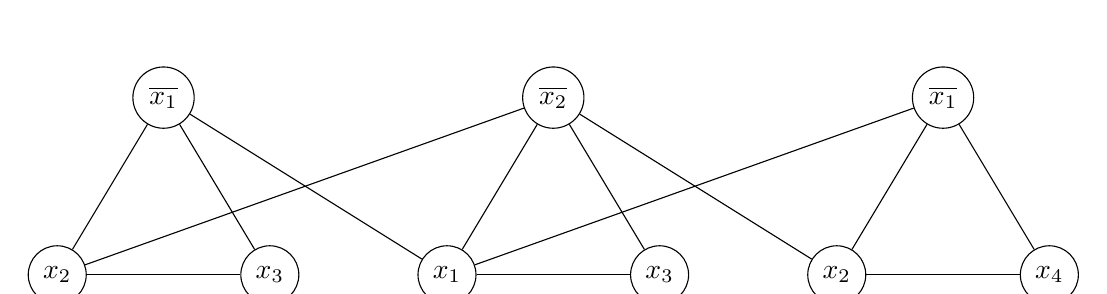
\begin{tikzpicture}  
          [scale=.9,auto=center,every node/.style={circle,draw=black}] % here, node/.style is the style pre-defined, that will be the default layout of all the nodes. You can also create different forms for different nodes.  
              
            \node (1) at (5, 2.5) {$\overline{x_1}$};  
            \node (2) at (3.5, 0) {$x_2$};  
            \node (3) at (6.5, 0) {$x_3$};

            \node (4) at (10.5, 2.5) {$\overline{x_2}$};
            \node (5) at (9, 0) {$x_1$};
            \node (6) at (12, 0) {$x_3$};

            \node (7) at (16, 2.5) {$\overline{x_1}$};
            \node (8) at (14.5, 0) {$x_2$};
            \node (9) at (17.5, 0) {$x_4$};
    
            \draw (1) -- (2);
            \draw (1) -- (3);
            \draw (2) -- (3);

            \draw (4) -- (5);
            \draw (4) -- (6);
            \draw (5) -- (6);

            \draw (7) -- (8);
            \draw (7) -- (9);
            \draw (8) -- (9);

            \draw (1) -- (5);
            \draw (5) -- (7);
            \draw (2) -- (4);
            \draw (4) -- (8);
            
        \end{tikzpicture} 
    \end{center}
    We claim that $\Phi$ is satisfiable if and only if $G$ contains 
    an independent set of size $k = |\Phi|$. 

    For the forward direction, consider any satisfying assignment for $\Phi$. 
    Then selecting one true literal from each clause (or triangle) will 
    give an independent set of size $k$. 

    Conversely, let $S$ be an independent set of size $k$. Then $S$ must 
    contain exactly one node in each triangle by construction. Set these 
    literals to ${\sf T}$ (and the remaining literals consistently). Then 
    all clauses in $\Phi$ are satisfied. This completes the proof. 
\end{pf}

The {\sc Vertex-Cover} problem is the following: given a graph $G = (V, E)$ 
and an integer $k$, is there a subset of $\leq k$ vertices such that 
each edge is incident to at least one vertex in the subset? 

The {\sc Set-Cover} problem is the following: given a set $U$ of elements, 
a collection $S$ of subsets of $U$, and an integer $k$, are there $\leq k$ 
of these subsets whose union is equal to $U$? 

\begin{theo}{theo:3.3}
    We have $\textsc{Vertex-Cover} \leq_P \textsc{Set-Cover}$. 
\end{theo}
\begin{pf}
    Given a {\sc Vertex-Cover} instance with the graph $G = (V, E)$ and 
    integer $k$, we construct a {\sc Set-Cover} instance $(U, S, k)$ that 
    has a set cover of size $k$ if and only if $G$ has a vertex cover of 
    size $k$. 

    We do this by setting the universe to be $U = E$, and include a 
    subset for each node $v \in V$ by 
    \[ S_v = \{e \in E : e \text{ incident to } v\}. \] 
    For example, consider the following graph $G$, which has a vertex 
    cover of size $2$ given by $\{c, f\}$. 
    \begin{center}
        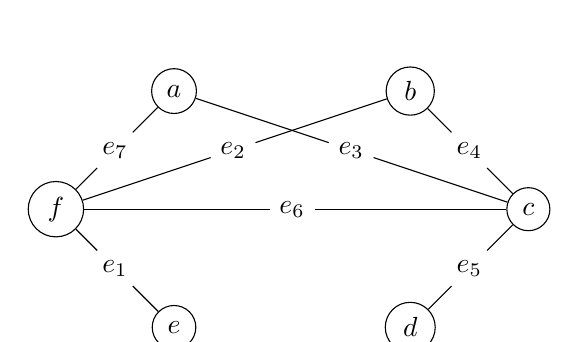
\begin{tikzpicture}              
            \node [circle, draw=black] (a) at (5, 3) {$a$};  
            \node [circle, draw=black] (b) at (8, 3) {$b$}; 
            \node [circle, draw=black] (c) at (9.5, 1.5) {$c$}; 
            \node [circle, draw=black] (d) at (8, 0) {$d$}; 
            \node [circle, draw=black] (e) at (5, 0) {$e$}; 
            \node [circle, draw=black] (f) at (3.5, 1.5) {$f$};

            \node (e1) at (4.25, 0.75) {$e_1$};
            \node (e2) at (5.75, 2.25) {$e_2$};
            \node (e3) at (7.25, 2.25) {$e_3$};
            \node (e4) at (8.75, 2.25) {$e_4$};
            \node (e5) at (8.75, 0.75) {$e_5$};
            \node (e6) at (6.5, 1.5) {$e_6$};
            \node (e7) at (4.25, 2.25) {$e_7$};

            \draw (e) -- (e1) -- (f);
            \draw (f) -- (e2) -- (b);
            \draw (a) -- (e3) -- (c);
            \draw (b) -- (e4) -- (c);
            \draw (c) -- (e5) -- (d);
            \draw (f) -- (e6) -- (c);
            \draw (f) -- (e7) -- (a);           
        \end{tikzpicture} 
    \end{center}
    Then we have universe $U = \{1, 2, 3, 4, 5, 6, 7\}$ with subsets 
    $S_a = \{3, 7\}$, $S_b = \{2, 4\}$, $S_c = \{3, 4, 5, 6\}$, 
    $S_d = \{5\}$, $S_e = \{1\}$, and $S_f = \{1, 2, 6, 7\}$. We can 
    see that $U = S_c \cup S_f$, so there is a set cover of size $2$. 

    Let us now show that $G = (V, E)$ contains a vertex cover of size $k$ 
    if and only if $U$ has a set cover of size $k$. 

    For the forward direction, let $X \subseteq V$ be a vertex cover of 
    size $k$ in $G$. Then $Y = \{S_v : v \in X\}$ is a set cover of size $k$. 
    Conversely, if $Y \subseteq S$ is a set cover of size $k$ for $U$, then 
    $X = \{v : S_v \in Y\}$ is a vertex cover of size $k$ in $G$. 
\end{pf}

\subsection{Intractability}\label{subsec:3.2}
There are three main types of problems. 
\begin{itemize}
    \item {\bf Decision problems.} Does there \emph{exist} a vertex cover of 
    size $\leq k$?
    \item {\bf Search problems.} \emph{Find} a vertex cover of size $\leq k$. 
    \item {\bf Optimization problems.} \emph{Find} a vertex cover of 
    \emph{minimum} size. 
\end{itemize}
In scheduling, we are mostly concerned with optimization problems. Notice that 
decision problems are in some sense easier than search problems, which are then 
easier than optimization problems. In particular, if the decision problem 
is intractible, then both the search and optimization problems are intractible.
Because of this, we will define {\bf P}, {\bf NP}, and {\bf EXP} using decision 
problems. A decision problem is essentially a yes or no question; we want to 
answer ``yes'' if the solution exists and ``no'' if it doesn't. 

\begin{defn}{defn:3.4}
    We denote by ${\bf P}$ the set of decision problems for which there 
    exists a polynomial time algorithm to solve it. 
\end{defn}

As we mentioned earlier, there are polynomial time algorithms for shortest 
path, primality testing, and linear programming, so these problems are all 
in {\bf P}. 

\begin{defn}{defn:3.5}
    \begin{itemize}
        \item An algorithm $C(s, t)$ is a {\bf certifier} for the problem $X$ if 
        for every string $s$, we have $s \in X$ if and only if there exists a 
        string $t$ such that $C(s, t)$ returns ``yes''. We call the string $t$ 
        the {\bf certificate} for the input $s$. 
        \item We denote by {\bf NP} the set of decision problems for which there exists 
        a polynomial time certifier. The certifier $C(s, t)$ is a 
        polynomial time algorithm, and the certificate $t$ for the input 
        $s$ is of polynomial size. 
    \end{itemize}
\end{defn}

\begin{exmp}{exmp:3.6}
    For the {\sc Sat} and {\sc 3-Sat} problems, the input is a propositional 
    formula $\Phi$ in CNF. A certificate for the input $\Phi$ is an 
    assignment of truth values to the boolean variables, and a certifier 
    checks that each clause in $\Phi$ has at least one true literal. 
    Thus, $\textsc{Sat} \in {\bf NP}$ and $\textsc{3-Sat} \in {\bf NP}$. 
\end{exmp}

Finally, we can define {\bf EXP}. 

\begin{defn}{defn:3.7}
    We denote by {\bf EXP} the set of decision problems for which there 
    exists an exponential time algorithm to solve it.
\end{defn}

\newpage
Now, we show that $\Poly \subseteq \NP \subseteq \EXP$. 

\begin{prop}{prop:3.8}
    We have $\Poly \subseteq \NP$. 
\end{prop}
\begin{pf}
    Consider a problem $X$ in $\Poly$. By definition, there exists a 
    polynomial time algorithm $A(s)$ which solves $X$ given any input $s$. 
    Then take the certificate $t = \eps$ to be the empty string, and 
    set the certifier to be $C(s, t) = A(s)$, which of course runs 
    in polynomial time. 
\end{pf}

\begin{prop}{prop:3.9}
    We have $\NP \subseteq \EXP$. 
\end{prop}
\begin{pf}
    Let $X$ be a problem in $\NP$. By definition, there exists a polynomial 
    time certifier $C(s, t)$ for $X$, whose certificate $t$ satisfies 
    $|t| \leq p(|s|)$ for some polynomial $p$ and any input string $s$. 
    To solve instance $s$, we run $C(s, t)$ on all strings $t$ with 
    $|t| \leq p(|s|)$. Return ``yes'' if and only if $C(s, t)$ returns 
    ``yes'' for any of these potential certificates. 
\end{pf}

It is a known fact that $\Poly \neq \EXP$, so we either have $\Poly \neq \NP$ 
or $\NP \neq \EXP$, or both. 

We now move on to {\bf NP}-completeness. We can think of these as the 
hardest problems in $\NP$. 

\begin{defn}{defn:3.10}
    A problem $Y \in \NP$ is called {\bf $\NP$-complete} if it has the property 
    that for every $X \in \NP$, we have $X \leq_P Y$. 
\end{defn}

The following proposition says that if we find even one problem $\NP$-complete 
problem $Y$ that is also in $\Poly$, then $\Poly = \NP$. Note that $\Poly = \NP$ 
is a famous conjecture, so we have of course not found one yet. It is commonly 
agreed upon that $\Poly \neq \NP$, but it is still an open problem.

\begin{prop}{prop:3.11}
    Suppose that $Y$ is $\NP$-complete. Then $Y \in \Poly$ if and only if 
    $\Poly = \NP$. 
\end{prop}
\begin{pf}
    For the backwards direction, notice that if $\Poly = \NP$, then 
    $Y \in \Poly$ since $Y \in \NP$. On the other hand, suppose $Y \in \Poly$. 
    Consider any problem $X \in \NP$. Since $X \leq_P Y$, we have $X \in \Poly$. 
    This implies that $\NP \subseteq \Poly$, and so $\Poly = \NP$. 
\end{pf}

The following proposition gives us a recipe for proving that a problem $Y$ 
is $\NP$-complete. 
\begin{enumerate}
    \item Show that $Y \in \NP$. 
    \item Choose an $\NP$-complete problem $X$ and prove that $X \leq_P Y$. 
\end{enumerate}

\begin{prop}{prop:3.12}
    If $X$ is $\NP$-complete, $Y \in \NP$, and $X \leq_P Y$, then 
    $Y$ is also $\NP$-complete. 
\end{prop}
\begin{pf}
    Consider any problem $W \in \NP$. Then $W \leq_P X$ by the definition 
    of $\NP$-completeness and $X \leq_P Y$ by assumption, so by transitivity, 
    we obtain $W \leq_P Y$. Since $W \in \NP$ is arbitrary, we have 
    that $Y$ is $\NP$-complete. 
\end{pf}

We now give some examples of $\NP$-complete problems. It is useful to know 
them as many scheduling problems are $\NP$-complete, and we can verify 
that they are indeed $\NP$-complete via reductions. 

\begin{theo}[Cook 1971, Levin 1973]{theo:3.13}
    The problem {\sc Sat} is $\NP$-complete. 
\end{theo}

\begin{exmp}{exmp:3.14}
    The following two problems are $\NP$-complete. 
    \begin{itemize}
        \item {\sc Partition}: Given $n$ positive integers $s_1, \dots, s_n$ 
        and $b = \frac12 \sum_{j=1}^n s_j$, does there exist a subset 
        $J \subseteq I = \{1, \dots, n\}$ such that 
        \[ b = \sum_{j\in J} s_j = \sum_{j\in I\setminus J} s_j? \] 
        \item {\sc $3$-Partition}: Given $3n$ positive integers 
        $s_1, \dots, s_{3n}$, and an integer $b$ satisfying 
        $\frac{b}{4} < s_j < \frac{b}{2}$ for all $j \in \{1, \dots, 3n\}$ 
        and $b = \frac1n \sum_{j=1}^{3n} s_j$, do there exist 
        $n$ pairwise disjoint three-element subsets $S_j \subseteq 
        \{1, \dots, 3t\}$ such that 
        \[ b = \sum_{j\in J_i} s_j \] 
        for all $j \in \{1, \dots, n\}$? 
    \end{itemize}
\end{exmp}

Next, we define what it means to be $\NP$-hard. 

\begin{defn}{defn:3.15}
    An $\NP$-hard problem is one such that every problem in $\NP$ 
    reduces to it in polynomial time. 
\end{defn}

Intuitively, $\NP$-hard problems are ``at least as hard as the hardest 
problems in $\NP$''. These problems are not necessarily in $\NP$, and they 
do not have to be decision problems. 
For instance, given an $\NP$-complete decision problem, the optimization 
problem corresponding to it is $\NP$-hard. 

There are two categories of $\NP$-hard problems.  
\begin{itemize}
    \item {\bf NP-hard in the ordinary sense.} We can reduce a known 
    $\NP$-hard problem to this problem using a polynomial time algorithm, 
    and we can find an optimal solution with an algorithm of pseudo-polynomial 
    time complexity. 
    \item {\bf NP-hard in the strong sense.} We can reduce a known 
    $\NP$-hard problem to this problem using a polynomial time algorithm, 
    even if the size of the largest parameter is polynomial in the 
    input size of the problem. 
\end{itemize}

In fact, it turns out that {\sc 3-Partition} (as defined in Example~\ref{exmp:3.14})
is $\NP$-hard in the strong sense, while {\sc Partition} is only $\NP$-hard 
in the ordinary sense. 

For our purposes, we can show that a scheduling problem is $\NP$-hard 
in the ordinary sense if {\sc Partition} (or a similar problem) can be 
reduced to this problem with a polynomial time algorithm, and there 
is an algorithm with pseudo-polynomial time complexity which solves the 
scheduling problem. 

On the other hand, we can show that a scheduling problem is $\NP$-hard 
in the strong sense if {\sc 3-Partition} (or a similar problem) can be 
reduced to this problem with a polynomial time algorithm. 

\subsection{PTAS for the Knapsack Problem}\label{subsec:3.3}
A {\bf polynomial time approximation scheme (PTAS)} is a
$(1 + \eps)$-approximation algorithm for any constant $\eps > 0$. 
While a PTAS produces arbitrarily high quality solutions, the consequence 
is that it trades off accuracy for time. Here, we will give a PTAS for the 
{\sc Knapsack} problem via rounding and scaling. 

In the {\sc Knapsack} problem, we are given $n$ objects and a knapsack. 
Each item $i$ has value $v_i > 0$ and weight $w_i > 0$. The knapsack 
has weight limit $W$. The goal is to fill the knapsack as to maximize 
the total value. 

First, we formulate the {\sc Knapsack} problem as a decision problem
and give a brief sketch that it is $\NP$-complete. 
Given a set $X$, weights $w_i \geq 0$, values $v_i \geq 0$, a weight 
limit $W$, and a target value $V$, is there a subset $S \subseteq X$ 
such that $\sum_{i\in S} w_i \leq W$ and $\sum_{i\in S} v_i \geq V$? 

The {\sc Subset-Sum} problem is the following: given $n$ natural numbers 
$w_1, \dots, w_n$ and an integer $W$, is there a subset that adds up to 
exactly $W$?

We know that {\sc Sat} is $\NP$-complete, and one can show that 
\[ \textsc{Sat} \leq_P \textsc{Subset-Sum} \leq_P \textsc{Knapsack}. \] 
\newpage
\section{More Single Machine Models} \label{sec:4}

\subsection{Maximum Lateness with Release Dates} \label{subsec:4.1}
We have already seen in Section~\ref{subsec:2.3} that there is a polynomial 
time algorithm to solve $(1\;\|\;L_{\max})$ instances. This was the 
Earliest Due Date (EDD) rule, which placed the jobs in increasing order of the 
due dates. We also saw that this was a special case of $(1 \mid \text{prec} 
\mid h_{\max})$, for which there was also an efficient algorithm, namely 
Lowest Cost Last (LCL). 

But what if we introduce release dates to the $(1\;\|\;L_{\max})$ problem? 
It turns out that this generalization, without preemption, is significantly 
harder than the problem where all jobs are available at time $0$. Moreover, 
the optimal schedule is not necessarily a non-delay schedule. It can be 
advantageous in this case to keep the machine idle before the release of a 
new job. 

\begin{theo}{theo:4.1}
    The problem $(1 \mid r_j \mid L_{\max})$ is strongly $\NP$-hard. 
\end{theo}
\begin{pf}
    This proof is based on the fact that {\sc $3$-Partition} (as described 
    in Example~\ref{exmp:3.14}) reduces to $(1 \mid r_j \mid L_{\max})$. 
    Suppose that we are given integers $a_1, \dots, a_{3t}, b$ such that 
    $\frac{b}{4} < a_j < \frac{b}{2}$ and $\sum_{j=1}^{3t} a_j = t \cdot b$. 
    We construct an instance of $(1 \mid r_j \mid L_{\max})$ with 
    $n = 4t - 1$ as follows: 
    \begin{itemize}
        \item For $j = 1, \dots, t-1$, we set $r_j = jb + (j-1)$, $p_j = 1$, 
        $d_j = jb + j$. 
        \item For $j = t, \dots, 4t-1$, we set $r_j = 0$, $p_j = a_{j-t+1}$, 
        and $d_j = tb + (t-1)$. 
    \end{itemize}
    Notice that a schedule with $L_{\max} \leq 0$ exists if and only if 
    every job $j \in \{1, \dots, t-1\}$ can be processed between 
    $r_j$ and $d_j = r_j + p_j$. This can be done if and only if the remaining 
    jobs can be partitioned over the $t$ intervals of length $b$, which can be 
    done if and only if {\sc $3$-Partition} has a solution. 
\end{pf}

The $(1 \mid r_j \mid L_{\max})$ problem is important because it often 
appears as a subproblem in heuristic procedures for flow shop and job shop 
problems. A branch and bound procedure $(1 \mid r_j \mid L_{\max})$ 
can be constructed as follows. The branching process may be based on the 
fact that schedules are developed starting from the beginning of the schedule. 
There is a single node at level $0$ which is the top of the tree. At this 
node, no job has been put into any position of the sequence yet. There are 
$n$ branches going down to $n$ nodes at level $1$. Each node at this level 
has a specific job put into the first position of the schedule. Then
at each node, there are $n-1$ jobs remaining whose position in the schedule 
has yet to be determined. Hence, there are $n-1$ arcs emanating from each 
node at level $1$ to level $2$, and there are $(n-1) \times (n-2)$ nodes at 
level $2$. We could continue in this way to enumerate all possible schedules. 

However, it is not necessary to consider every remaining job as a possible 
candidate for the next position. If the jobs $j_1, \dots, j_{k-1}$ 
are scheduled as the first $k-1$ jobs at a node at level $k-1$, then 
we only need to consider job $j_k$ if 
\[ r_{j_k} < \min_{\ell \in J} \left( \max(t, r_\ell) + p_\ell \right), \] 
where $J$ denotes the set of jobs not yet scheduled and $t$ denotes the 
time job $j_k$ is supposed to start. The reason for this condition is because 
if job $j_k$ does not satisfy this inequality, then selecting the job 
which minimizes the right-hand side instead of $j_k$ does not increase the 
value of $L_{\max}$. Therefore, the branching rule is fairly easy. 

There are several ways in which bounds for nodes can be obtained. 
One easy lower bound for a node at level $k-1$ can be established by 
scheduling the remaining jobs $J$ according to the \emph{preemptive} 
EDD rule which is known to be optimal for $(1 \mid r_j, \text{prmp} \mid 
L_{\max})$, and thus provides a lower bound for the problem at hand. 
If a preemptive EDD rule results in a non-preemptive schedule, then 
all nodes with a higher lower bound may be disregarded. 

\begin{exmp}{exmp:4.2}
    Consider the following instance of $(1 \mid r_j \mid L_{\max})$ with 
    $n = 4$ jobs. 
    \begin{align*}
        \begin{array}{c|cccc} 
            j & 1 & 2 & 3 & 4 \\ \hline 
            p_j & 4 & 2 & 6 & 5 \\ 
            r_j & 0 & 1 & 3 & 5 \\ 
            d_j & 8 & 12 & 11 & 10 
        \end{array}
    \end{align*}
    At level $1$ of the search tree, there are four nodes, namely 
    $(1, *, *, *)$, $(2, *, *, *)$, $(3, *, *, *)$, and $(4, *, *, *)$. 
    Notice that we may discard the nodes $(3, *, *, *)$ and 
    $(4, *, *, *)$ immediately. Indeed, we have $\min_{\ell\in \{1, 2, 3, 4\}} 
    (\max(t, r_\ell) + p_\ell) = 3$ with $\ell = 2$, and we see that 
    $r_3 \geq 3$ and $r_4 \geq 3$. 

    Computing a lower bound for node $(1, *, *, *)$ according to the 
    preemptive EDD rule results in a schedule where job $3$ is processed 
    during the interval $[4, 5]$, job $4$ is processed during $[5, 10]$, 
    job $3$ again during $[10, 15]$, and job $2$ during $[15, 17]$. 
    Then $L_{\max} = 5$ for this schedule, and so $5$ is a lower bound 
    for the node $(1, *, *, *)$. A similar computation shows that a lower 
    bound for the node $(2, *, *, *)$ is $7$. 

    Consider now the node $(1, 2, *, *)$ at level $2$. The lower bound 
    for this node is $6$ and is determined by the non-preemptive 
    schedule $1, 2, 4, 3$. Next, looking at the node $(1, 3, *, *)$ 
    at level $2$, the lower bound is $5$ and is determined by the 
    non-preemptive schedule $1, 3, 4, 2$. Since the lower bound for node 
    $(1, *, *, *)$ is $5$ and the lower bound for $(2, *, *, *)$ is 
    greater than $5$, it follows that the schedule $1, 3, 4, 2$ is optimal. 
\end{exmp}

The problem $(1 \mid r_j, \text{prec} \mid L_{\max})$ can be handled in a similar 
way. From an enumeration point of view, it is even easier than the problem 
without precedence constraints since many schedules can be ruled out 
immediately. 

\subsection{Number of Tardy Jobs} \label{subsec:4.2}
Recall that $U_j = 0$ if the job is timely and $U_j = 1$ if the job is late. 
The goal of the problem $(1\;\|\;\sum U_j)$ is to minimize the number of 
tardy jobs. This objective may at first appear somewhat artificial and 
seems to be of no practical interest. However, in the real world, it is a 
performance measure that is often monitored. It is equivalent to the 
percentage of on time shipments.

Notice that it does not matter how late a job is; the only 
determining factor is if it is late or not. A solution to this problem can 
be represented as a partition of the jobs into sets $S_1$ and $S_2$, where 
$S_1$ is the set of jobs meeting their due dates in Earliest Due Date (EDD)
order, and $S_2$ is the set of late jobs in an arbitrary order (since the 
amount of lateness is irrelevant).  

\begin{lemma}{lemma:4.3}
    Let OPT denote the optimal value for a given instance of $(1\;\|\;\sum U_j)$.
    If the sequence given by the EDD rule has a late job, then $\text{OPT} \geq 1$. 
\end{lemma}
\begin{pf}
    Let $k$ be the first late job in the EDD sequence. Then we have 
    \[ C_k = \sum_{i\in[k]} p_i > d_k = \max_{i\in[k]} d_i. \] 
    Consider any schedule $S$. Let $\ell$ be the last of the jobs in $[k]$ in 
    $S$. Then the completion time of $\ell$ in $S$ is at least $\sum_{i\in[k]} 
    p_i > d_\ell$, so $\ell$ is a late job in $S$. 
\end{pf}

\begin{algo}[Moore-Hodgson]{algo:4.4}
    \begin{enumerate}
        \item Enumerate the jobs in EDD order. 
        \item Set $S_1 \gets \varnothing$ and $t \gets 0$. 
        \item for $j=1$ to $n$ do: 
        \begin{itemize}[\label{}]
            \item Set $S_1 \gets S_1 \cup \{j\}$ and $t \gets t + p_j$. 
            \item if $t > d_j$ then: 
            \begin{itemize}[\label{}]
                \item Find a job $k$ with the largest $p_k$ value in $S_1$. 
                \item Set $S_1 \gets S_1 \setminus \{k\}$ and $t \gets t - p_k$. 
            \end{itemize}
            endif
        \end{itemize}
        endfor
    \end{enumerate}
\end{algo}

The principle of the Moore-Hodgson algorithm is that we schedule the jobs by the EDD 
rule, and when a job gets late, we rescue the situation by throwing out the job with 
the highest processing time. All removed jobs are considered late, and the remaining 
ones are timely. This algorithm runs in $O(n\log n)$ time. 

\begin{exmp}{exmp:4.5}
    Consider the following instance of $(1 \;\|\; \sum U_j)$ with $n = 5$ jobs, 
    where the jobs are already in EDD order.  
    \begin{align*}
        \begin{array}{c|ccccc}
            j   & 1 & 2  & 3  & 4  & 5 \\ \hline 
            p_j & 7 & 8  & 4  & 6  & 6 \\ 
            d_j & 9 & 17 & 18 & 19 & 21
        \end{array}
    \end{align*}
    We can initially schedule jobs $1$ and $2$, which will both be timely. However, 
    once we schedule job $3$, we see that it will be late, since $t = 19 > 18 = d_3$.
    \begin{verbatim}
        |---1---|---2----|-3--|
        0       7        15   19
    \end{verbatim}
    \vspace{-1em}
    Therefore, we toss out job $2$ which has the highest processing time of $p_2 = 8$
    and continue. We can schedule job $4$ just fine, but job $5$ will be late with 
    $t = 23 > 21 = d_5$. 
    \begin{verbatim}
        |---1---|-3--|--4---|--5---|
        0       7    11     17     23
    \end{verbatim}
    \vspace{-1em}
    This time, we toss out job $1$ since it has the highest processing time of $p_1 = 7$. 
    Then we obtain $S_1 = \{3, 4, 5\}$ and $S_2 = \{1, 2\}$, so $\text{OPT} = 2$ for 
    this instance. 
\end{exmp}

The following lemma is the key to proving that the Moore-Hodgson algorithm is 
optimal for $(1\;\|\;\sum U_j)$. We will assume that the jobs are already scheduled 
in EDD. 

\begin{lemma}{lemma:4.6}
    Suppose there is at least one late job in the EDD sequence $1, \dots, n$. 
    Let $k$ be the first late job in the EDD sequence, and let $m$ be the first 
    job rejected by the Moore-Hodgson algorithm. Then there is an optimal 
    schedule which rejects $m$. 
\end{lemma}
\begin{pf}
    Consider any optimal schedule $\pi$. Let $R_\pi \subseteq [n]$ denote 
    the subset of rejected (late) jobs, and let $A_\pi = [n] \setminus R_\pi$ 
    denote the set of timely jobs. By Lemma~\ref{lemma:4.3}, we may assume that 
    $\pi$ schedules the jobs of $A_\pi$ in EDD order, followed by the 
    jobs of $R_\pi$ in arbitrary order. 

    If $m \in R_\pi$, we are done. So suppose that $m \notin R_\pi$. 
    By Lemma~\ref{lemma:4.3}, there is a job $r \in [k]$ other than $m$ 
    that has been rejected. Consider the schedule $\sigma$ that sequences 
    the jobs in $A_\sigma = (A_\pi \setminus \{m\}) \cup \{r\}$ in EDD 
    order first, followed by the jobs in $[n] \setminus A_\sigma = 
    (R_\pi \setminus \{r\}) \cup \{m\}$ in arbitrary order. We will show that 
    $\sigma$ schedules all jobs in $A_\sigma$ on time. This will mean that 
    $\sigma$ is an optimal schedule since $|R_\sigma| = |R_\pi|$, 
    and by construction, $\sigma$ rejects $m$.

    First, the jobs in $A_\sigma \cap [k-1]$ are completed on time 
    since the EDD rule completes all jobs in $[k-1]$ on time. Next, 
    if $k \in A_\sigma$, then its completion time is at most 
    \[ \sum_{i\in[k] \setminus \{m\}} p_i \leq 
    \sum_{i\in[k-1]} p_i \leq d_{k-1} \leq d_k, \] 
    where the first inequality follows from the choice of $m$ by the 
    Moore-Hodgson algorithm which ensures that $p_m = 
    \max_{i\in[k]} p_i \geq p_k$. Finally, compared to the schedule $\pi$, 
    the completion times of the jobs in $A_\sigma \setminus [k] = 
    A_\pi \setminus [k]$ have been changed in the new schedule $\sigma$
    by $p_r - p_m \leq 0$, so these jobs are also on time. 
\end{pf}
 
\begin{theo}{theo:4.7}
    The Moore-Hodgson algorithm gives an optimal schedule for 
    $(1\;\|\;\sum U_j)$. 
\end{theo}
\begin{pf}
    We proceed by induction on $\text{OPT}$ over all instances of the problem. 

    If an instance has $\text{OPT} = 0$, then by Lemma~\ref{lemma:4.3}, the 
    Moore-Hodgson algorithm outputs the EDD sequence with no late jobs. 

    Suppose now that $I$ is an instance with $\text{OPT}(I) \geq 1$ late 
    jobs. Let $I'$ be obtained from $I$ by deleting the first job $m$ 
    which is rejected by the Moore-Hodgson algorithm. By Lemma~\ref{lemma:4.6}, 
    we have $\text{OPT}(I') = \text{OPT}(I) - 1$. By the induction hypothesis, 
    the algorithm finds an optimal schedule $S'$ for $I'$. The algorithm 
    for $I$ outputs the schedule $S$ such that $S$ is the same as $S'$ 
    except that job $m$ is added at the end as a rejected job. Clearly, 
    $S$ has at most $\text{OPT}(I') + 1 = \text{OPT}(I)$ rejected jobs 
    and hence is optimal. 
\end{pf}

\subsection{Total Tardiness} \label{subsec:4.3}
In practice, minimizing the number of tardy jobs $\sum U_j$ cannot be the 
only objective to measure how due dates are being met. Only minimizing 
the number of late jobs will force some jobs to have to wait for an 
unacceptably long time to complete. If we instead minimize the total 
tardiness, it is less likely that the wait for any given job will be 
unacceptably long. 

The problem $(1\;\|\;\sum T_j)$ has received an enormous amount of attention 
in literature. For many years, its computational complexity remained open; 
its $\NP$-hardness was only established recently in 1990. Since 
$(1\;\|\;\sum T_j)$ is $\NP$-hard in the ordinary sense, it allows for a 
pseudo-polynomial time algorithm based on dynamic programming. The 
algorithm is based on two preliminary results. 

\begin{lemma}{lemma:4.8}
    If $p_j \leq p_k$ and $d_j \leq d_k$, then there exists an optimal schedule 
    in which job $j$ is scheduled before job $k$. 
\end{lemma}
\begin{pf}
    We leave the proof as an exercise. This is a standard interchange 
    argument. 
\end{pf}

This type of result is useful when an algorithm has to be developed for
a problem that is $\NP$-hard. Such a result, often referred to as a 
{\bf dominance result} or {\bf elimination criterion}, often allows one to
disregard a fairly large number of sequences. Such a dominance result may also 
be thought of as a set of precedence constraints on the jobs. The more 
precedence constraints created through such dominance results, the easier the 
problem becomes.

In the following lemma, the sensitivity of an optimal sequence to the due
dates is considered. We consider two problem instances, both of which have 
$n$ jobs with processing times $p_1, \dots, p_n$. The first instance has 
due dates $d_1, \dots, d_n$. Let $k$ be a fixed job, and let $\hat C_k$ 
be the latest completion time of job $k$ among all optimal schedules. 
Then we set the due dates for the second instance to be 
\[ \hat d_j = \begin{cases}
    d_j, & \text{if } j \neq k, \\ 
    \max(d_k, \hat C_k), & \text{if } j = k.
\end{cases} \] 
In particular, we are only changing one piece of data, namely the 
due date of job $k$. 

\begin{lemma}{lemma:4.9}
    Any optimal sequence with respect to the second instance with due dates 
    $\hat d_1, \dots, \hat d_n$ is also optimal for the first instance 
    with due dates $d_1, \dots, d_n$. 
\end{lemma}
\begin{pf}
    We first introduce some notation. Let $\hat S$ be an optimal sequence 
    such that job $k$ has largest completion time $\hat C_k$ among 
    all optimal sequences. For an arbitrary sequence $S$, we let 
    $V(S)$ be the objective value according to the first instance 
    where job $k$ has due date $d_k$, and $V'(S)$ be the objective 
    value according to the second instance where job $k$ has due date 
    $\hat d_k$. 

    Let $S'$ be any optimal sequence for the second instance. Then we have 
    $V'(\hat S) \geq V'(S')$ since $S'$ is optimal for the second instance. 
    Moreover, we observe that 
    \[ V'(\hat S) = V(\hat S) - (\hat C_k - d_k), \] 
    or equivalently, $V(\hat S) - V'(\hat S) = \hat C_k - d_k$. Finally, 
    when we switch objectives, the most improvement we can get is 
    $\hat C_k - d_k$, so we deduce that 
    \begin{align*}
        V(S') &\leq V'(S') + (\hat C_k - d_k) \\ 
        &= V'(S') + V(\hat S) - V'(\hat S) \\ 
        &\leq V(\hat S).
    \end{align*}
    This means that $S'$ is also optimal for the first instance, so we are done. 
\end{pf}

Lemma~\ref{lemma:4.9} is quite a technical result, and it requires the 
knowledge of all optimal sequences for the first instance. 
For now, we will assume that the jobs are scheduled in EDD order 
so that $d_1 \leq \cdots \leq d_n$, and job $k$ is such that 
$p_k = \max(p_1, \dots, p_n)$. In particular, this is the job with 
the $k$-th smallest due date and largest processing time. It follows from 
Lemma~\ref{lemma:4.8} that there exists an optimal sequence in which 
jobs $1, \dots, k-1$ all appear in some order before job $k$. Of the remaining 
$n-k$ jobs, some may appear before job $k$ while some may appear after job $k$. 
The following lemma focuses on the placement of these remaining jobs. 

\begin{lemma}{lemma:4.10}
    There is an integer $\delta$ with $0 \leq \delta \leq n-k$ such that there 
    is an optimal sequence $S$ in which job $k$ is preceded by all jobs $j$ 
    with $j \leq k + \delta$ and followed by all jobs $j$ with $j > k + \delta$. 
\end{lemma}
\begin{pf}
    We only give a brief sketch here. In some optimal schedule, the jobs 
    $1, \dots, k-1$ are positioned before 
    job $k$ due to the dominance criterion from Lemma~\ref{lemma:4.8}. 
    From Lemma~\ref{lemma:4.9}, we can increase $d_k$ such that some other 
    jobs $k+1, \dots, k+\delta$ are positioned before job $k$ due to the 
    dominance criterion. 
\end{pf}

Lemma~\ref{lemma:4.10} tells us an optimal sequence looks like the concatenation 
of three subsets of jobs, namely 
\begin{enumerate}[(i)]
    \item jobs $1, \dots, k-1, k+1, \dots, k+\delta$ in some order, followed by 
    \item job $k$, followed by 
    \item jobs $k+\delta+1, \dots, n$ in some order. 
\end{enumerate}
The completion time of job $k$ under this schedule is 
\[ C_k(\delta) = \sum_{j\leq k+\delta} p_j. \] 
For the entire sequence to be optimal, it is clear that the first and third 
subsets must be optimally sequenced within themselves. This is the heart of 
a dynamic programming approach that determines an optimal sequence for a 
larger set of jobs after having determined optimal sequences for proper 
subsets of the larger set. 

We define $J(j, \ell, k)$ to be the set of all jobs in the set $\{j, \dots, \ell\}$ 
with processing time at most $p_k$, but $k \notin J(j, \ell, k)$. 
Note that here, $k$ does not necessarily have to be the job with highest processing 
time. Then, we define $V(J(j, \ell, k), t)$ to be the total tardiness of 
the jobs $J(j, \ell, k)$ in an optimal sequence that starts at time $t$. 
We now state the dynamic programming algorithm. 

\begin{algo}[Dynamic Programming for Total Tardiness]{algo:4.11}
    The initial conditions are $V(\varnothing, t) = 0$ and 
    $V(\{j\}, t) = \max(0, t + p_j - d_j)$ for all jobs $j$ and $t \geq 0$. 
    We have the recursive relation 
    \[ V(J(j, \ell, k), t) = \min_{\delta} \{V(J(j, k'+\delta, k'), t)
    + \max(0, C_{k'}(\delta) - d_{k'}) + V(J(k'+\delta+1, \ell, k'), 
    C_{k'}(\delta))\}, \] 
    where job $k'$ is such that $p_{k'} = \max_{j'\in J(j,\ell, k)} p_{j'}$. 
    The optimal value is then given by $V(\{1, \dots, n\}, 0)$. 
\end{algo}

Note that there are at most $O(n^3)$ subsets of jobs $J(j, \ell, k)$ and 
$\sum p_j$ possible values of $t$. This means that there are 
$O(n^3 \sum p_j)$ recursive equations. Each recursion takes $O(n)$ time, 
so the total running time of the dynamic programming approach is 
$O(n^4 \sum p_j)$, which is pseudo-polynomial. 

\begin{exmp}{exmp:4.12}
    We run our dynamic programming algorithm on an example. Consider 
    the following instance of $(1\;\|\;\sum T_j)$ with $n = 5$ jobs. 
    \begin{align*}
        \begin{array}{c|ccccc}
            j & 1 & 2 & 3 & 4 & 5 \\ \hline 
            p_j & 121 & 79 & 147 & 83 & 130 \\ 
            d_j & 260 & 266 & 266 & 336 & 337 
        \end{array}
    \end{align*}
    We see that job $3$ has the largest processing time, giving us 
    $0 \leq \delta \leq 5 - 3 = 2$. Then we have 
    \[ V(\{1, 2, 3, 4, 5\}, 0) = \min\begin{cases} 
        V(J(1, 3, 3), 0) + 81 + V(J(4, 5, 3), 347), & \text{for } \delta = 0, \\ 
        V(J(1, 4, 3), 0) + 164 + V(J(5, 5, 3), 430), & \text{for } \delta = 1, \\ 
        V(J(1, 5, 3), 0) + 294 + V(\varnothing, 560), & \text{for } \delta = 2. 
    \end{cases} \] 
    We see that $V(J(1, 3, 3), 0) = 0$ via the sequences $1, 2$ and $2, 1$. 
    The dominance rule tells us that the sequences $1, 2, 4$ and $2, 1, 4$ 
    are optimal for the jobs $J(1, 4, 3)$ with $V(J(1, 4, 3), 0) = 0$, 
    and similarly, the sequences $1, 2, 4, 5$ and $2, 1, 4, 5$ are optimal for 
    $J(1, 5, 3)$ with $V(J(1, 5, 3), 0) = 76$.

    On the other hand, we have 
    \[ V(J(4, 5, 3), 347) = (347 + 83 - 336) + (347 + 83 + 130 - 337) = 317 \] 
    for the sequence $4, 5$, and $V(J(5, 5, 3), 430) = 430 + 130 - 337 = 223$.

    Putting everything together, we obtain 
    \[ V(\{1, 2, 3, 4, 5\}, 0) = 
    \min\{0 + 81 + 317, 0 + 164 + 223, 76 + 294 + 0\}
    = \min\{398, 387, 370\} = 370. \] 
    The sequences that attain this value are $1, 2, 4, 5, 3$ and $2, 1, 4, 5, 3$.    
\end{exmp}

Since $(1\;\|\;\sum T_j)$ is $\NP$-hard, we cannot hope to find a polynomial 
time algorithm to solve arbitrary instances of it. However, we can give an FPTAS
to obtain a solution that is close to optimal, using a similar approach 
as we did for the {\sc Knapsack} problem in Section~\ref{subsec:3.4}. 

First, we will give some lower and upper bounds for total tardiness. 
\begin{itemize}
    \item Recall that the EDD rule produces a schedule with optimal 
    maximum lateness. In particular, this also produces a schedule 
    with optimal maximum tardiness. 
    \item Clearly, at least one job in a schedule has the maximum tardiness. 
    Then the total tardiness of an optimal schedule is at least the 
    optimal maximum tardiness. 
    \item The total tardiness of the EDD schedule is at least the optimal 
    maximum tardiness, but at most $n$ times the optimal maximum tardiness. 
\end{itemize}
Let $\sum T_j(\text{EDD})$ denote the total tardiness under the EDD schedule, 
and let $T_{\max}(\text{EDD}) = \max(T_1, \dots, T_n)$ be the maximum 
tardiness under the EDD schedule. For an optimal schedule $\text{OPT}$, we have 
\[ T_{\max}(\text{EDD}) \leq \sum T_j(\text{OPT}) \leq \sum T_j(\text{EDD}) 
\leq n \cdot T_{\max}(\text{EDD}). \] 
Let $V(J, t)$ be the minimum total tardiness of the job subset $J$ 
assuming that processing begins at time $t$. There is a time $t^*$ 
such that $V(J, t) = 0$ for all $t \leq t^*$ and $V(J, t) > 0$ for all 
$t > t^*$. Then we have $V(J, t^* + \delta) \geq \delta$ for all 
$\delta \geq 0$. By executing the pseudo-polynomial dynamic programming 
approach described in Algorithm~\ref{algo:4.11}, one only has to compute 
$V(J, t)$ for 
\[ \max\{0, t^*\} \leq t \leq t^* + n \cdot T_{\max}(\text{EDD}). \] 
Substituting $\sum p_j$ in the overall running time of the dynamic 
programming algorithm by $n \cdot T_{\max}(\text{EDD})$ yields a 
new bound of $O(n^5 \cdot T_{\max}(\text{EDD}))$. 

Now, rescale the processing times and due dates via $p'_j = 
\lfloor p_j/K \rfloor$ and $d'_j = d_j/K$ for some factor $K > 0$. 
Let $S$ be an optimal schedule for the rescaled problem. We let 
$\sum T_j^*(S)$ denote the total tardiness of the schedule $S$ with 
respect to the processing times $Kp'_j \leq p_j$ and due dates $d_j$. 
Let $\sum T_j(S)$ denote the total tardiness of the schedule $S$ with 
respect to the original processing times $p_j$ and due dates $d_j$. 
From the fact that $Kp'_j \leq p_j < K(p'_j + 1)$, it follows that 
\[ \sum T_j^*(S) \leq \sum T_j(\text{OPT}) \leq \sum T_j(S) < 
\sum T_j^*(S) + \frac{Kn(n+1)}{2}. \] 
This chain of inequalities implies that 
\[ \sum T_j(S) - \sum T_j(\text{OPT}) < \frac{Kn(n+1)}{2}. \] 
If $K$ is chosen such that 
\[ K = \frac{2\eps}{n(n+1)} \cdot T_{\max}(\text{EDD}), \] 
then we obtain 
\[ \sum T_j(S) - \sum T_j(\text{OPT}) < \eps \cdot T_{\max}(\text{EDD}). \] 
Moreover, for this choice of $K$, the time bound 
$O(n^5 \cdot T_{\max}(\text{EDD})/K)$ becomes $O(n^7/\eps)$, making 
our approximation scheme fully polynomial. We summarize the FPTAS 
as follows. 

\begin{algo}[Total Tardiness FPTAS]{algo:4.13}
    \begin{enumerate}[(1)]
        \item Apply EDD in order to determine $T_{\max}(\text{EDD})$. 
        If $T_{\max}(\text{EDD}) = 0$, then $\sum T_j(\text{OPT}) = 0$ 
        and EDD gives an optimal schedule, so stop. Otherwise, set 
        \[ K = \frac{2\eps}{n(n+1)} \cdot T_{\max}(\text{EDD}). \] 
        \item Rescale the processing times and due dates via 
        $p'_j = \lfloor p_j/K \rfloor$ and $d'_j = d_j/K$. 
        \item Apply Algorithm~\ref{algo:4.11} to the rescaled data. 
    \end{enumerate}
\end{algo}

\subsection{Weighted Number of Late Jobs} \label{subsec:4.4}
The generalization of the problem $(1\;\|\;\sum U_j)$ with additional weights 
is known to be $\NP$-hard. This can be shown via a reduction from 
{\sc $3$-Partition}. A popular heuristic for this problem is the WSPT rule, 
but even that can perform very badly. As usual, we cannot hope to find a 
polynomial time algorithm which solves $(1\;\|\;\sum w_j U_j)$. 

\begin{exmp}{exmp:4.14}
    Consider the following instance of $(1 \mid d_j = d \mid \sum w_j U_j)$ with 
    $n = 3$ jobs and equal due dates. 
    \begin{align*}
        \begin{array}{c|ccc}
            j & 1 & 2 & 3 \\ \hline 
            p_j & 11 & 9 & 90 \\ 
            d_j & 100 & 100 & 100 \\ 
            w_j & 12 & 9 & 89
        \end{array}
    \end{align*}
    Then the WSPT rule fails: it gives the schedule $1, 2, 3$ which has 
    objective value $89$. The optimal schedules for this example are 
    $2, 3, 1$ and $3, 2, 1$, which both have objective value $12$. 
\end{exmp}

In fact, the {\sc Knapsack} problem is equivalent to the special case 
$(1 \mid d_j = d \mid \sum w_j U_j)$ where all due dates are equal. 
Indeed, we can think of the due date $d$ as the weight of the knapsack, 
the processing times $p_j$ as the weight of the individual items, 
and the weights $w_j$ as their values. We then want to minimize the value 
of the items we are throwing out of the knapsack, which is the same 
as maximizing the value of the items inside the knapsack. 

In this section, our goal is to come up with some dynamic programming 
approaches to solve $(1\;\|\;\sum w_j U_j)$ in pseudo-polynomial time. 
We then construct an FPTAS using one of the dynamic programming schemes. 

First, we will introduce some notation. Consider an instance of 
$(1\;\|\;\sum w_j U_j)$ where all weights $w_j \geq 0$ are integer. 
We assume that the jobs are indexed by the EDD sequence. 
\begin{itemize}
    \item We call $S$ a {\bf feasible} set of jobs if every job in $S$ 
    can be completed on time starting at time $0$. 
    \item We define $w(S) = \sum_{j\in S} w_j$ and $p(S) = \sum_{j\in S} p_j$. 
\end{itemize}

{\bf Approach 1.} We define $T(i, \hat w)$ to be the minimum completion 
time of a feasible subset $S$ of $[i] = \{1, \dots, i\}$ with weight 
$\geq \hat w$. We can think of $\hat w$ as a ``target'' weight. 
In other words, $T(i, \hat w)$ is the minimum completion time of a 
chosen subset of the jobs $\{1, \dots, i\}$ such that all jobs in the 
chosen subset are timely (that is, there are no late jobs in an EDD ordering 
of the chosen subset) and moreover, the total weight of the jobs in the 
chosen subset is $\geq \hat w$.

We set $T(i, \hat w) = \infty$ if no such feasible set exists, 
$T(0, 0) = 0$, and $T(0, \hat w) = \infty$ for all $\hat w > 0$. Then 
the recurrence relation is given by 
\[ T(i, \hat w) = \begin{cases}
    \min\{T(i-1, \hat w), p_i + T(i-1, \hat w - w_i)\}, & \text{if } 
    p_i + T(i-1, \hat w - w_i) \leq d_i, \\ 
    T(i-1, \hat w), & \text{otherwise.} 
\end{cases} \] 
In the computed table for $T(i, \hat w)$, there are $n+1$ rows corresponding 
to $i = 0, \dots, n$ where $n$ is the number of jobs, and $\sum w_j + 1$ 
corresponding to the potential total weights $\hat w = 0, \dots, \sum w_j$. 
From the table, we can then find the optimal solution to the 
$(1\;\|\;\sum w_j U_j)$ instance in $O(\sum w_j)$ time.

We can actually do slightly better. If $w^*$ is the maximum value of 
$w$ such that $T(i, w^*)$ is finite, then we can compute the table for 
$T(i, \hat w)$ in $O(nw^*)$ time and find the optimal solution from the 
table in $O(w^*)$ time. So the dynamic programming algorithm runs in time 
$O(nw^*)$. 

{\bf Approach 2.} This is the approach we will use for our FPTAS. We define 
$Q(i, \hat w)$ to be the minimum completion time of a feasible subset $S$ 
of $[i]$ such that $w([i] \setminus S) \leq \hat w$. In other words, 
$Q(i, \hat w)$ is the minimum completion time of a chosen subset of the jobs 
$\{1, \dots, i\}$ such that all of the jobs in the chosen subset are timely 
(that is, there are no late jobs in an EDD ordering of the chosen subset)
and moreover, the sum of the weights of the remaining jobs in 
$\{1, \dots, i\}$ is $\leq \hat w$. 

We define $Q(0, \hat w) = 0$ for all $\hat w \geq 0$ and $Q(0, \hat w) 
= \infty$ for all $\hat w < 0$. Then the recurrence relation is given by 
\[ Q(i, \hat w) = \begin{cases}
    \min\{Q(i-1, \hat w - w_i), p_i + Q(i-1, \hat w)\}, & \text{if } 
    p_i + Q(i-1, \hat w) \leq d_i, \\ 
    Q(i-1, \hat w - w_i), & \text{otherwise.}
\end{cases} \]
In essence, this is the complement to the first approach. But why do we 
prefer this one instead? This is because it is slightly more efficient. 
We do not need to compute all of the entries of the table like in the 
first approach; we only need to start at $\hat w = 0$ and stop when 
we reach the minimum value $w^{**}$ such that $Q(i, w^{**})$ is finite. 
Observe that this minimum value $w^{**}$ is the same as the optimal value 
to the $(1\;\|\;\sum w_j U_j)$ instance. In many cases, the value of 
$w^{**}$ is much smaller than that of $w^*$ above. 

Our FPTAS then uses an extension of the above observation. If we can compute a 
lower bound $\text{LB}$ on $\text{OPT}$ such that $\text{LB} \leq 
\text{OPT} \leq n \cdot \text{LB}$, then we could replace $w^{**}$ above 
by $n \cdot \text{LB}$. We design the FPTAS by scaling and rounding the 
weights, and then applying our second dynamic programming approach above
with $Q(i, \hat w)$. This is quite similar to the FPTAS of the {\sc Knapsack} 
problem. 

There are two key building blocks for the FPTAS for $(1\;\|\;\sum w_j U_j)$. 
\begin{enumerate}[(1)]
    \item We need a lower bound $\text{LB}$ on $\text{OPT}$ computable in 
    polynomial time such that $\text{LB} \leq \text{OPT} \leq n \cdot \text{LB}$.
    \item We need an algorithm (based on dynamic programming) which computes 
    the optimal value and runs in time  polynomial in $n$ and $\text{LB}$. 
\end{enumerate}
We address (1) by solving the problem $(1\;\|\;\max_j w_jU_j)$ on the 
same instance. This can be done by applying the LCL algorithm 
(Algorithm~\ref{algo:2.10}) to the functions 
\[ h_j(C_j) = \begin{cases} 
    0, & \text{if } C_j \leq d_j, \\ 
    w_j, & \text{if } C_j > d_j. 
\end{cases} \] 
We also have the following result, and we leave its proof as an exercise. 

\begin{prop}{prop:4.15}
    For any schedule $S$, we have 
    \[ \max_j w_j U_j^S \leq \sum_j w_j U_j^S \leq n \cdot \max_j w_j U_j^S. \] 
    Moreover, if $S^*$ is an optimal schedule for $(1\;\|\;\max_j w_jU_j)$, then 
    \[ \max_j w_j U_j^{S^*} \leq \text{OPT} \leq n \cdot \max_j w_j U_j^{S^*}, \] 
    where $\text{OPT}$ is the optimal value for the $(1\;\|\;\sum w_j U_j)$ instance. 
\end{prop}

We set $\text{LB}$ to be the optimal value for the $(1\;\|\;\max_j w_j U_j)$ 
instance. Our scale and round step is straightforward. Given an error 
parameter $\eps > 0$, let the scaling parameter be $\delta = \eps \cdot 
\text{LB}/n$. We define $w'_j = \lfloor w_j/\delta \rfloor$ for all jobs $j$. 
It is easy to see that $w_j/\delta - 1 \leq w'_j \leq w_j/\delta$. 

We apply the second dynamic programming algorithm to the rounded instance 
with the weights $w'$. The running time is polynomial in $n$ and 
$\text{LB}'$ where $\text{LB}' = \text{LB}/\delta = n/\eps$ because 
the optimal value of the rounded instance is $\leq n \cdot \text{LB}'$.

For the rounded instance, let $\text{OPT}'$ denote the optimal value. 
Let $A'$ be the set of late jobs in an optimal schedule, so $w'(A') = 
\text{OPT}'$. Let $A^*$ be the set of late jobs in an optimal schedule for 
the original instance so that $w(A^*) = \text{OPT}$. 

We claim that $w(A') \leq (1+\eps) \text{OPT}$. This follows from applying some
inequalities we have stated earlier and the fact that $w'(A') \leq w'(A^*)$ 
since $A'$ is optimal for the weights $w'$. Indeed, we have 
\begin{align*} 
    w(A') &= \sum_{j\in A'} w_j \leq \sum_{j\in A'} (\delta w'_j + \delta) \\
    &\leq \delta w'(A') + n\delta \\ 
    &\leq \delta w'(A^*) + n\delta \\
    &\leq w(A^*) + \eps \cdot \text{LB} \\ 
    &\leq (1 + \eps) w(A^*) \\ 
    &= (1 + \eps) \text{OPT}. 
\end{align*}
Thus, we see that our algorithm is an FPTAS. 
\newpage
\section{Advanced Single Machine Models} \label{sec:5}

\subsection{Total Earliness and Tardiness} \label{subsec:5.1}
One could imagine a situation where an earliness penalty is incurred. For 
example, if one needs to go to convocation in a different city a week from now, 
they wouldn't want to go immediately as they would need to pay for rent 
or parking.  We define the earliness of a job $j$ by $E_j = \max(0, d_j - C_j)$.
Note that unlike the performance measures we have discussed so far, 
earliness is non-regular because it is decreasing with respect to 
completion time. 

In this section, we cover a generalization of the total tardiness 
problem. We will focus on the objective 
\[ \sum_{j=1}^n E_j + \sum_{j=1}^n T_j. \] 
Intuitively, this problem is harder than total tardiness, which is known to be 
$\NP$-hard. Therefore, we will focus on the special case where all 
jobs have the same due date $d_j = d$. 

An optimal schedule for this special case has some useful properties. For 
example, it is easily shown that there is no idleness between any two jobs 
for an optimal schedule, as one could close the gap by shifting jobs 
later if they are early, or shifting jobs earlier if they are late. 
Moreover, it is possible that an optimal schedule does not start processing 
the jobs immediately at time $0$. Indeed, by the previous property, 
an increase of $d$ would increase the starting time of the first job if 
$d$ is sufficiently large. 

We also observe that we can divide any sequence of jobs into 
two disjoint sets and possibly one additional job. One set consists of the jobs 
that are completed early so that $C_j \leq d$, and we will denote it by $J_1$. 
The other set consists of the jobs that are started late, and we will denote it 
by $J_2$. There may be another job which is started early but 
completed late. 

\begin{prop}{prop:5.1}
    There is an optimal sequence in which one job is completed exactly 
    at time $d$. 
\end{prop}
\begin{pf}
    We proceed by contradiction. Suppose there is no such schedule. Then
    there is always one job that starts its processing before time $d$ and 
    completes its processing after time $d$. Call this job $j^*$. 
    Let $|J_1|$ denote the number of jobs that are early and $|J_2|$ 
    denote the number of jobs that are late. If $|J_1| < |J_2|$, then we 
    can shift the entire schedule to the left in such a way that job $j^*$
    completes its processing exactly at time $d$. This implies that the 
    total tardiness decreases by $|J_2|$ times the length of the shift, 
    while the total earliness increases by $|J_1|$ times the length of 
    the shift. Clearly, the objective value is reduced. The case 
    where $|J_1| > |J_2|$ can be treated in a similar way. 

    The case where $|J_1| = |J_2|$ is somewhat special. In this case, there 
    are many optimal schedules, of which only two satisfy the property 
    given in the lemma. 
\end{pf}

Due to Proposition~\ref{prop:5.1}, we can avoid the situation where we have the 
additional job in the middle altogether. In particular, there is an optimal 
schedule such that the first job starts at time $0$ or later, the jobs in $J_1$ 
scheduled first according to Longest Processing Time (LPT), and the jobs in $J_2$
are scheduled last according to Shortest Processing Time (SPT). In this 
sense, the schedule is shaped like a ``V''. Note that for a schedule of the 
above form, say $1, \dots, n$, the total earliness is 
\[ \sum_{j\in J_1} E_j = 0 \cdot p_1 + 1 \cdot p_2 + 2 \cdot 
p_3 + \cdots + (|J_1| - 1) \cdot p_{|J_1|}, \] 
while the total tardiness is 
\[ \sum_{j\in J_2} T_j = 1 \cdot p_{|J_1|+|J_2|} + 2 \cdot 
p_{|J_1|+|J_2|-1} + \cdots + |J_2| \cdot p_{|J_1|+1}. \] 
For an instance in which all optimal schedules start processing the first job
some time after $t = 0$ (that is, the due date $d$ is sufficiently large), 
the following algorithm yields the optimal allocations of jobs to sets 
$J_1$ and $J_2$. We assume that the jobs are ordered such that $p_1 \geq 
p_2 \geq \cdots \geq p_n$. 

\begin{algo}[Minimizing Total Earliness and Tardiness with Loose Due Date]{algo:5.2}
    {\sc Step 1.} Assign job $1$ to set $J_1$. Initialize $k = 2$. 

    {\sc Step 2.} Assign job $k$ to set $J_1$ and job $k+1$ to set $J_2$, 
    or vice versa. 

    {\sc Step 3.} If $k+2 \leq n-1$, then increase $k$ by $2$ and go back to 
    Step 2. If $k+2 = n$, assign job $n$ to either set $J_1$ or set $J_2$ 
    and stop. If $k+2 = n+1$, then all jobs have been assigned, so we stop. 
\end{algo}

This algorithm is somewhat flexible in its assignment of jobs to sets $J_1$ and 
$J_2$. It can be implemented in a way that in the optimal assignment, the 
total processing time of the jobs assigned to $J_1$ is minimized. Given the 
total processing time of the jobs in $J_1$ and the due date $d$, it can be 
verified easily whether the machine indeed must remain idle before it starts 
processing its first job.

If the due date $d$ is tight and it is necessary to start processing 
a job at time $0$, then the problem is $\NP$-hard. The following heuristic 
which assigns the $n$ jobs to the $n$ positions in the sequence can be 
very effective, but does not always yield an optimal sequence. Again, we 
assume that $p_1 \geq p_2 \geq \cdots \geq p_n$.  

\begin{algo}[Minimizing Total Earliness and Tardiness with Tight Due Date]{algo:5.3}
    {\sc Step 1.} Initialize $\tau_1 = d$ and $\tau_2 = \sum_{j=1}^n p_j - d$. 
    Set $k = 1$.  

    {\sc Step 2.} If $\tau_1 > \tau_2$, then assign job $k$ to the first 
    unfilled position in the sequence and decrease $\tau_1$ by $p_k$. 
    If $\tau_1 < \tau_2$, then assign job $k$ to the last unfilled position 
    in the sequence and decrease $\tau_2$ by $p_k$. 

    {\sc Step 3.} If $k < n$, then increase $k$ by $1$ and go back to Step 2. 
    If $k = n$, then stop. 
\end{algo}

We give an example of this heuristic in action. 

\begin{exmp}{exmp:5.4}
    Consider the following example with $6$ jobs and common due date $d = 180$. 
    \begin{align*}
        \begin{array}{c|cccccc}
            j & 1 & 2 & 3 & 4 & 5 & 6 \\ \hline 
            p_j & 106 & 100 & 96 & 22 & 20 & 2
        \end{array}
    \end{align*}
    Applying the heuristic yields the following results. 
    \begin{align*}
        \begin{array}{c|c|c|c}
            \tau_1 & \tau_2 & \text{Assignment} & \text{Sequence} \\ \hline 
            180 & 166 & \text{Job $1$ placed first} & 1, *, *, *, *, * \\ 
            74 & 166 & \text{Job $2$ placed last} & 1, *, *, *, *, 2 \\ 
            74 & 66 & \text{Job $3$ placed first} & 1, 3, *, *, *, 2 \\ 
            -22 & 66 & \text{Job $4$ placed last} & 1, 3, *, *, 4, 2 \\ 
            -22 & 44 & \text{Job $5$ placed last} & 1, 3, *, 5, 4, 2 \\
            -22 & 24 & \text{Job $6$ placed last} & 1, 3, 6, 5, 4, 2 \\  
        \end{array}
    \end{align*}
\end{exmp}

To end this section, we discuss some other versions of total 
earliness and tardiness problems. 
\begin{itemize}

    \item Consider the objective $\sum w'E_j + \sum w''T_j$ where all 
    due dates are equal with $d_j = d$. All jobs have exactly the same 
    cost function, but the earliness penalty $w'$ and the tardiness 
    penalty $w''$ are not the same. All the previous properties and
    algorithms can be generalized relatively easily to take the 
    difference between $w'$ and $w''$ into account. 

    \item Consider the more general objective $\sum w'_j E_j + \sum w''_j T_j$ 
    with $d_j = d$ for all jobs $j$. In this case, the shapes of the cost 
    functions of the jobs are different. The LPT-SPT sequence described above 
    is not necessarily optimal. The first part of the sequence must now be 
    ordered according to Weighted Longest Processing Time first (WLPT), 
    which is in increasing order of $w_j/p_j$. The second part of the 
    sequence is ordered by Weighted Shortest Processing Time first (WSPT), 
    which we are already familiar with. 

    \item Consider the model with the objective function $\sum w'E_j + \sum w''T_j$
    where we do not assume that the due dates are equal. It is clear that this 
    case is $\NP$-hard as it is a more general model of the one we discussed in
    Section~\ref{subsec:4.3}. This problem has an additional level of complexity. Because of
    the different due dates, it may not necessarily be optimal to process the 
    jobs one after another without interruption; it may be necessary to have 
    idle times between the processing of consecutive jobs. Therefore, this 
    problem has two aspects: one concerning the sequencing of the jobs, 
    and the other concerning the idle time between the jobs. Approaches 
    for this problem are typically based either on dynamic programming 
    or branch and bound. However, given a predetermined sequence, the timing of 
    the processing of the jobs (and therefore also the idle times) can be 
    determined in polynomial time. This can also be applicable in a more 
    general setting, which we will describe next. 

    \item The most general setting has objective $\sum w'_j E_j + 
    \sum w''_j T_j$ where the jobs have different due dates and weights. 
    This problem is strongly $\NP$-hard since it is harder than 
    $(1~||~\sum w_j T_j)$, which is also known to be strongly $\NP$-hard.
    But again, given a predetermined sequence of the jobs, the timing 
    of the jobs can be determined in polynomial time. However, we will not 
    go into detail about this. 

\end{itemize} 

\subsection{Primary and Secondary Objectives} \label{subsec:5.2}
In practice, a scheduler is often concerned with more than one objective. 
For example, one might want to minimize inventory costs and meet due dates. 
It would then be of interest, for instance, to find a schedule that minimizes a 
combination of $\sum C_j$ and $L_{\max}$. 

In many cases, there is more than one optimal schedule that minimizes a 
given objective. A scheduler may then wish to consider the set of all 
schedules that are optimal with respect to one objective (which 
we will call the primary objective), and then search within this set of 
schedules for the schedule that is best with regard to a secondary objective. 
If the primary objective is $\gamma_1$ and the secondary objective is 
$\gamma_2$, then such a problem is denoted by 
$(\alpha~|~\beta~|~\gamma_1^{(1)}, \gamma_2^{(2)})$.

We begin with the simple example $(1~||~\sum C_j^{(1)}, L_{\max}^{(2)})$ 
where the primary objective is the total completion time and the secondary 
objective is the maximum lateness. If there are no jobs with identical 
processing times, then there is exactly one schedule that minimizes the 
total completion time (namely the one obtained by SPT), so there is 
no freedom to minimize $L_{\max}$. If there are jobs with identical processing 
times, then there are multiple schedules that minimize the total completion 
time. A set of jobs with identical processing times is preceded by a job with a 
strictly shorter processing time and followed by a job with a strictly longer
processing time. Jobs with identical processing times have to be processed 
one after another, but the key is that they may be done in any order. 
Then to minimize $L_{\max}$, we can put these jobs with identical processing 
times in EDD order. We can refer to this rule as SPT/EDD, since the jobs are 
first scheduled according to SPT and ties are broken according to EDD. This 
rule can generalized to the case where the primary objective is 
the total weighted completion time $\sum w_j C_j$. 

Consider now the problem $(1~||~\sum L_{\max}^{(1)}, C_j^{(2)})$, which 
has the same two objectives with reversed priorities. We know that 
the EDD rule minimizes $L_{\max}$; suppose that the value of this minimum 
$L_{\max}$ is $z$. Then the original problem can be transformed to 
another equivalent problem. By creating a new set of due dates 
$\overline{d_j} = d_j + z$, we see that these due dates are now deadlines. 
The problem is to find a schedule which minimizes $\sum C_j$ subject to 
the constraint that every job is completed by its deadline. We denote 
this problem by $(1~|~\text{hard } d_j~|~\sum C_j)$. The algorithm 
for finding the optimal schedule is based on the following result. 

\begin{lemma}{lemma:5.5}
    There exists a schedule that minimizes $\sum C_j$ in which job $k$ 
    is scheduled last if and only if 
    \begin{enumerate}[(1)]
        \item $\overline{d_k} \geq \sum_{j=1}^n p_j$, and 
        \item $p_k \geq p_\ell$ for all jobs $\ell$ such that 
        $\overline{d_\ell} \geq \sum_{j=1}^n p_j$. 
    \end{enumerate}
\end{lemma}
\begin{pf} 
    Assume towards a contradiction that job $k$ is not scheduled last. 
    There is a set of jobs that is scheduled after job $k$, and 
    some job $\ell$ that is scheduled last. Note that job $\ell$ 
    must satisfy condition (1) for otherwise it would not meet its due date. 
    This means that job $\ell$ does not satisfy condition (2) and 
    so $p_\ell < p_k$. After swapping jobs $k$ and $\ell$, the sum of the 
    completion times of jobs $k$ and $\ell$ decreases, and the sum of the 
    completion times of jobs scheduled between $k$ and $\ell$ also decreases. 
    Hence, the original schedule that positioned job $\ell$ last could not have 
    minimized $\sum C_j$. 
\end{pf}

In the following algorithm, $J^c$ represents the set of jobs that have 
not been scheduled yet. 

\begin{algo}[Minimizing Total Completion Time with Deadlines]{algo:5.6}
    {\sc Step 1.} Set $k = n$, $\tau = \sum_{j=1}^n p_j$, and $J^c = \{1, \dots, n\}$. 

    {\sc Step 2.} Find a job $k^* \in J^c$ such that $\overline{d_{k^*}} \geq \tau$ 
    and $p_{k^*} \geq p_\ell$ for all jobs $\ell \in J^c$ such that 
    $\overline{d_\ell} \geq \tau$. Put job $k^*$ in position $k$ of the sequence. 

    {\sc Step 3.} Decrease $k$ by $1$, decrease $\tau$ by $p_{k^*}$, and 
    delete job $k^*$ from $J^c$. 

    {\sc Step 4.} If $k \geq 1$, then go back to Step 2. Otherwise, stop. 
\end{algo}

We give a simple example of the use of this backward algorithm. 

\begin{exmp}{exmp:5.7}
    Consider the following instance of $5$ jobs. 
    \begin{align*}
        \begin{array}{c|ccccc}
            j & 1 & 2 & 3 & 4 & 5 \\ \hline 
            p_j & 4 & 6 & 2 & 4 & 2 \\ 
            d_j & 10 & 12 & 14 & 18 & 18
        \end{array}
    \end{align*}
    For ease of notation, we will let $\hat J(\tau) = \{\ell \in J^c : 
    \overline{d_\ell} \geq \tau\}$ be the set of eligible jobs that have 
    not been scheduled yet. We start with $\tau = \sum_{j=1}^5 p_j = 18$, 
    and applying the algorithm yields the following results. 
    \begin{align*}
        \begin{array}{c|c|c|c} 
            \text{Iteration} & \tau & \hat J(\tau) & k^* \\ \hline 
            1 & 18 & \{4, 5\} & 4 \\ 
            2 & 14 & \{3, 5\} & 3 \text{ or } 5 \\ 
            3 & 12 & \{2, 5\} \text{ or } \{2, 3\} & 2 \\ 
            4 & 6 & \{1, 5\} \text{ or } \{1, 3\} & 1 \\ 
            5 & 2 & \{5\} \text{ or } \{3\} & 5 \text{ or } 3            
        \end{array}
    \end{align*}
    Thus, we obtain two optimal schedules, which are $5, 1, 2, 3, 4$ and 
    $3, 1, 2, 5, 4$. 
\end{exmp}

It can be shown that even when preemptions are allowed, the optimal schedules 
are non-preemptive for the $(1~|~\text{hard } d_j~|~\sum C_j)$ problem. We can 
also assume feasibility of the problem in general as it can be checked easily 
using the EDD rule. 

Finally, we note that a fairly large number of problems of the form 
$(1~|~\beta~|~\gamma_1^{(1)}, \gamma_2^{(2)})$ have been studied in the 
literature. Very few of them can be solved in polynomial time. However, 
problems of the type $(1~|~\beta~|~\sum w_j C_j^{(1)}, \gamma_2^{(2)})$ 
tend to be easy based on the analysis of the $(1~||~\sum C_j^{(1)}, 
L_{\max}^{(2)})$ problem we discussed at the beginning of the lecture. 
We will see one such example on Assignment 6.

\subsection{Parametric Analysis of Multiple Objectives} \label{subsec:5.3}
Suppose that we have the two objectives $\gamma_1$ and $\gamma_2$. If 
the overall objective is $\theta_1 \gamma_1 + \theta_2 \gamma_2$ where 
$\theta_1$ and $\theta_2$ are the weights of the two objectives, then 
we can denote the scheduling problem by $(1~|~\beta~|~\theta_1 \gamma_1 
+ \theta_2 \gamma_2)$. Multiplying both weights by the same constant 
does not change the problem, so we may assume without loss of generality 
that $\theta_1 + \theta_2 = 1$. For this section, we will focus on a 
specific class of schedules. 

\begin{defn}{defn:5.8}
    A schedule is called {\bf Pareto optimal} if it is not possible to 
    decrease the value of one objective without increasing the value of 
    the other. 
\end{defn}

All Pareto optimal schedules can be represented by a set of points in the 
$(\gamma_1, \gamma_2)$ plane. This set of points illustrates the tradeoffs 
between the two objectives. Consider the two objectives we analyzed in the 
previous section, namely $\sum C_j$ and $L_{\max}$. The two cases 
we covered are the two extreme points of the tradeoff curve. Note that 
if $\theta_1 \to 0$ and $\theta_2 \to 1$, then 
\[ (1~|~\beta~|~\theta_1\gamma_1 + \theta_2\gamma_2) \to 
(1~|~\beta~|~\gamma_2^{(1)}, \gamma_1^{(2)}), \] 
while if $\theta_2 \to 0$ and $\theta_1 \to 1$, then 
\[ (1~|~\beta~|~\theta_1\gamma_1 + \theta_2\gamma_2) \to 
(1~|~\beta~|~\gamma_1^{(1)}, \gamma_2^{(2)}). \] 
We will now focus on generating all Pareto optimal schedules for the 
problem $(1~||~\theta_1 \sum C_j + \theta_2 L_{\max})$. 

On one end of the extremes is the $(1~||~\sum L_{\max}^{(1)}, \sum C_j^{(2)})$ 
problem, which could be solved using a more complicated backward algorithm
where we have $L_{\max} = L_{\max}(\text{EDD})$. 

On the other end, we have the $(1~||~\sum C_j^{(1)}, L_{\max}^{(2)})$ problem, 
where the total completion time was minimized by the SPT rule and ties were 
broken by EDD. We denoted this strategy by SPT/EDD, and we easily see that 
$L_{\max} = L_{\max}(\text{SPT/EDD})$ in this case. It is clear that 
\[ L_{\max}(\text{EDD}) \leq L_{\max}(\text{SPT/EDD}). \] 
The algorithm that generates all Pareto optimal solutions in the tradeoff 
curve contains two loops. One series of steps in the algorithm (the inner 
loop) is an adaptation of Algorithm~\ref{algo:5.6}. In addition to the optimal 
schedule with a maximum allowable $L_{\max}$, these steps determine 
the minimum increment $\delta$ in the $L_{\max}$ that would allow for a 
decrease in the minimum $\sum C_j$. The second (outer) loop of the algorithm 
contains the structure that generates all the Pareto optimal points.
The outer loop calls the inner loop at each Pareto optimal point to generate a 
schedule at that point and also to determine how to move to the next efficient 
point. The algorithm starts out with the EDD schedule that generates the first
Pareto optimal point in the upper left part of the trade-off curve. It 
determines the minimum increment in the $L_{\max}$ needed to achieve a 
reduction in $\sum C_j$. Given this new value of $L_{\max}$, it uses 
Algorithm~\ref{algo:5.6} to determine the schedule which minimizes 
$\sum C_j$, and proceeds to determine the next increment. This goes on 
until the algorithm reaches $L_{\max}(\text{SPT/EDD})$. 

\begin{algo}[Tradeoffs between Total Completion Time and 
    Maximum Lateness]{algo:5.9}
    {\sc Step 1.} Set $r = 1$. Set $L_{\max} = L_{\max}(\text{EDD})$ and 
    $\overline{d_j} = d_j + L_{\max}$. 

    {\sc Step 2.} Set $k = n$ and $J^c = \{1, \dots, n\}$. Set 
    $\tau = \sum_{j=1}^n p_j$ and $\delta = \tau$. 

    {\sc Step 3.} Find a job $j^* \in J^c$ such that $\overline{d_{j^*}} \geq \tau$ 
    and $p_{j^*} \geq p_\ell$ for all jobs $\ell \in J^c$ such that 
    $\overline{d_\ell} \geq \tau$. Put job $j^*$ in position $k$ of the 
    sequence. 

    {\sc Step 4.} If there is no job $\ell$ such that $\overline{d_\ell} < 
    \tau$ and $p_\ell > p_{j^*}$, then go to Step 5. Otherwise, let 
    \[ \delta^{**} = \min\{\tau - \overline{d_\ell} : 
    \text{jobs $\ell$ such that $\overline{d_\ell} < \tau$ and 
    $p_\ell > p_{j^*}$}\} \] 
    and set $\delta = \min\{\delta, \delta^{**}\}$. 

    {\sc Step 5.} Decrease $k$ by $1$, decrease $\tau$ by $p_{j^*}$, 
    and delete job $j^*$ from $J^c$. If $k \geq 1$, then go to Step 3. 
    If $k = 0$, then go to Step 6. 

    {\sc Step 6.} Set $L_{\max} = L_{\max} + \delta$. If $L_{\max} 
    > L_{\max}(\text{SPT/EDD})$, then stop. Otherwise, set 
    $r = r+1$, $\overline{d_j} = \overline{d_j} + \delta$, and 
    go to Step 2. 
\end{algo}

The outer loop consists of Steps 1 and 6, while the inner loop consists of 
Steps 2, 3, 4, and 5. Steps 2, 3, and 5 represent an adaptation of 
Algorithm~\ref{algo:5.6}, while Step 4 computes the minimum increment 
in the $L_{\max}$ needed to achieve a subsequent reduction in $\sum C_j$. 

It can be shown that the number of Pareto optimal solutions is bounded 
above by $\binom{n}{2} + O(1)$, which is $O(n^2)$. Generating one Pareto optimal 
solution can be done in $O(n\log n)$ time. Therefore, the total computation 
time of Algorithm~\ref{algo:5.9} is $O(n^3\log n)$. 

We now give an example of the use of the above algorithm. 

\begin{exmp}{exmp:5.10}
    Consider the following set of $5$ jobs. 
    \begin{align*}
        \begin{array}{c|ccccc}
            j & 1 & 2 & 3 & 4 & 5 \\ \hline 
            p_j & 1 & 3 & 6 & 7 & 9 \\ 
            d_j & 30 & 27 & 20 & 15 & 12
        \end{array}
    \end{align*}
    The EDD sequence is $5, 4, 3, 2, 1$ with $L_{\max}(\text{EDD}) = 2$ 
    and total completion time $98$. The SPT/EDD sequence is $1, 2, 3, 4, 5$ with 
    $L_{\max}(\text{SPT/EDD}) = 14$ and total completion time $58$. 

    We give an example of one full iteration of the inner loop.
    \begin{itemize}
        \item Initially, we have $k = 5$, $\tau = \sum_{j=1}^5 p_j = 26$, and 
        so the set of eligible jobs to put at the end of the sequence is $\{1, 2\}$.
        Since job $2$ has the largest processing time, we place it last. 
        Then we have $\delta^{**} = \tau - \overline{d_3} = 26 - 22 = 4$ and so
        $\delta = 4$. 
        \item Next, we have $k = 4$, $\tau = 23$, and job $1$ is the 
        only eligible job. Then $\delta^{**} = 23 - 22 = 1$ and $\delta = 1$. 
        \item Then, we have $k = 3$, $\tau = 22$, and the only eligible job is 
        job $3$. We then have $\delta^{**} = \tau - \overline{d_4} = 22 - 17 = 5$.
        \item For the next iteration of the inner loop, we have $k = 2$, $\tau = 16$, 
        and job $4$ is the only eligible job. Then $\delta^{**} = \tau 
        - \overline{d_5} = 16 - 12 = 4$.
        \item Finally, we pick job $5$ at the end, and obtain the Pareto optimal 
        schedule $5, 4, 3, 1, 2$ with $\delta = 1$.
    \end{itemize} 
    The full results are given in the following table. 
    \begin{align*}
        \begin{array}{c|c|c|c|c|c}
            \text{Iteration} & \sum C_j & L_{\max} & \text{Pareto optimal schedule} 
            & \text{current } \tau + \delta & \delta \\ \hline 
            1 & 96 & 2 & 5, 4, 3, 1, 2 & 32~29~22~17~14 & 1 \\ 
            2 & 77 & 3 & 1, 5, 4, 3, 2 & 33~30~23~18~15 & 2 \\ 
            3 & 75 & 5 & 1, 4, 5, 3, 2 & 35~32~25~20~17 & 1 \\ 
            4 & 64 & 6 & 1, 2, 5, 4, 3 & 36~33~26~21~18 & 2 \\ 
            5 & 62 & 8 & 1, 2, 4, 5, 3 & 38~35~28~23~20 & 3 \\ 
            6 & 60 & 11 & 1, 2, 3, 5, 4 & 41~38~31~26~23 & 3 \\ 
            7 & 58 & 14 & 1, 2, 3, 4, 5 & 44~41~34~29~26 & \text{STOP} 
        \end{array}
    \end{align*} 
\end{exmp}

However, when one would consider the objective $\theta_1 \sum C_j + \theta_2 
L_{\max}$, certain Pareto optimal schedules may never be optimal, 
no matter what the weights are. 

Consider the generalization $(1~||~\theta_1 \sum w_j C_j + \theta_2 L_{\max})$. 
It is clear that the two extreme points of the tradeoff curve can be determined 
in polynomial time using WSPT/EDD and EDD. However, even though the two 
endpoints of the tradeoff curve can be analyzed in polynomial time, the 
problem with arbitrary weights $\theta_1$ and $\theta_2$ is $\NP$-hard. 

The tradeoff curve that corresponds to the example in this section has the
shape of a staircase. This shape is fairly common in a single machine 
environment with multiple objectives, especially when preemptions are not 
allowed. However, in other machine environments such as parallel machines, 
smoother curves may occur, especially when preemptions are allowed.
We will not cover more parametric analysis in this course though. 
\newpage
\section{Parallel Machine Models} \label{sec:6}

\subsection{Makespan without Preemptions} \label{subsec:6.1}

\subsubsection{List Scheduling and Longest Processing Time} \label{subsubsec:6.1.1}
The makespan is not a very interesting objective for a single machine. 
However, for parallel machine models, minimizing the makespan has the effect 
of balancing the load over the various machines, which is an important 
objective in practice. Recall that we denote this by $(P_m~\|~C_{\max})$.

One can see that $(P_2~\|~C_{\max})$ is $\NP$-hard via a reduction from 
\textsc{Partition}. Indeed, consider an instance of \textsc{Partition}, 
where we are given $a_1, \dots, a_t \in \Z^+$ and want to find a subset 
$S \subseteq \{1, \dots, t\}$ such that 
\[ \sum_{j\in S} a_j = \frac12 \sum_{j=1}^t a_j = b. \] 
Let $n = t$ be the number of jobs each with processing time $p_j = a_j$. Then 
it is easy to check that there is a schedule with optimal value at most 
$\frac12 \sum_{j=1}^n p_j$ if and only if there is a solution to the 
\textsc{Partition} instance. 

Over the years, there have been many heuristics developed for 
$(P_m~\|~C_{\max})$. We focus on one such heuristic, and present it by 
discussing some history on how this algorithm was developed. First, we 
take a look at the list scheduling rule, which runs in $O(n\log m)$ time 
using a priority queue for the loads. 

\begin{algo}[List Scheduling]{algo:6.1}
    Given $n$ jobs in some arbitrary order, assign job $j$ to machine $i$ 
    whose load is smallest so far for each $j \in [n]$. 
\end{algo}

There are two obvious lower bounds on OPT, namely 
\begin{enumerate}[(1)]
    \item $\text{OPT} \geq \max_{j\in[n]} p_j$ since the jobs are not preemptive, and 
    \item $\text{OPT} \geq \frac1m \sum_{j=1}^n p_j$ because at least one machine must 
    have load which is at least the average. 
\end{enumerate}
We shall denote the load of a machine $i$ by $L(i) = p(S(i)) = 
\sum_{j\in S(i)} p_j$, where $S(i)$ is the set of jobs assigned to machine $i$.

\begin{theo}{theo:6.2}
    Algorithm~\ref{algo:6.1} is a $2$-approximation for $(P_m~\|~C_{\max})$. 
\end{theo}
\begin{pf}
    Let $i$ denote the machine which the highest load determining the objective 
    value. Let $j$ be the last job scheduled on machine $i$. When job $j$ was 
    assigned to machine $i$, it had the smallest load. Its load before the 
    assignment was $L(i) - p_j$, and thus $L(i) - p_j \leq L(k)$ for all 
    $1 \leq k \leq m$. Summing up this inequality over all $k$ and 
    dividing by $m$, we obtain 
    \[ L(i) - p_j \leq \frac1m \sum_{k=1}^m L(k) = \frac1m \sum_{j=1}^n p_j 
    \leq \text{OPT}. \] 
    We deduce that $L(i) = (L(i) - p_j) + p_j \leq 2 \cdot \text{OPT}$. 
\end{pf}

Is this analysis tight? That is, are there any examples where the factor 
is as bad as $2$? The answer is essentially yes. Suppose there are $m$ machines.
Take $m(m-1)$ jobs each with processing time $1$, and let the last job 
in the order have processing time $m$. Then the list scheduling algorithm 
will try to balance the $m(m-1)$ jobs among the $m$ machines first. Then 
we are forced to run the last job with processing time $m$ last on one 
of the machines, and that machine has load $2m - 1$. An optimal schedule 
instead places the job with processing time $m$ on its own machine, 
and balances the load of the $m(m-1)$ jobs between the remaining $m-1$ 
machines. This gives a makespan of $m$ instead. 

It can be shown that Algorithm~\ref{algo:6.1} is in fact a 
$(2 - \frac1m)$-approximation, and the above example shows that this is 
exactly a tight bound. 

We now consider the {\bf Longest Processing Time first (LPT)} rule.

\begin{algo}[LPT]{algo:6.3}
    Sort the $n$ jobs in decreasing order of $p_j$, then run 
    Algorithm~\ref{algo:6.1}.
\end{algo}

This is equivalent to the following procedure: at time $t = 0$, 
assign the $m$ longest jobs to the $m$ machines. Afterwards, 
whenever a machine is freed, the longest job among those not yet processed is 
put on the machine. This heuristic tries to place the shorter jobs more towards 
the end of the schedule, where they can be used for balancing the loads.

\begin{exercise}{exercise:6.4}
    Show that if an optimal schedule results in at most two jobs on any
    machine, then LPT is optimal.
\end{exercise}

Under the LPT rule in the case that $n \geq m+1$, we also have an additional 
lower bound on OPT. This is given by $\text{OPT} \geq 2p_{m+1}$ because 
at least one machine must run two jobs by the time it gets to the 
$(m+1)$-th job, and that machine has load at least $2p_{m+1}$ as the 
jobs are in decreasing order of the processing times. 

\begin{theo}{theo:6.5}
    Algorithm~\ref{algo:6.3} is a $\frac32$-approximation for $(P_m~\|~C_{\max})$.
\end{theo}
\begin{pf}
    This is the same proof as Theorem~\ref{theo:6.2}, except that we now 
    have $p_j \leq p_{m+1} \leq \text{OPT}/2$. 
\end{pf}

This is actually a very crude bound. We give a more sophisticated analysis 
showing that the LPT rule is a $(\frac43 - \frac{1}{3m})$-approximation, 
and that this bound is tight.  

\begin{theo}{theo:6.6}
    For $(P_m~\|~C_{\max})$, we have 
    \[ \frac{C_{\max}(\text{LPT})}{C_{\max}(\text{OPT})} \leq 
    \frac43 - \frac{1}{3m}. \] 
\end{theo}
\begin{pf}
    We proceed by contradiction. Suppose there are counterexamples with 
    ratio strictly larger than $\frac43 - \frac1{3m}$. Among these 
    counterexamples, there must be a counterexample with the least 
    number of jobs. 

    Suppose this smallest counterexample has $n$ jobs. This counterexample 
    has a useful property: under LPT, the shortest job is the last job 
    to start its processing and also the last job to finish its processing. 
    To see why this is true, note that by the definition of LPT, 
    the shortest job is the last to finish its processing. On the other hand, 
    if this job was not last to finish processing, then the deletion of 
    this smallest job would result in a counterexample with fewer jobs since 
    $C_{\max}(\text{LPT})$ remains the same while $C_{\max}(\text{OPT})$ 
    either stays the same or decreases, which is a contradiction to our 
    assumption that our counterexample was minimal. 

    Therefore, for our smallest counterexample, the starting time of the 
    shortest job is $C_{\max}(\text{LPT}) - p_n$. At this point, all other 
    machines are busy, so we have 
    \[ C_{\max}(\text{LPT}) - p_n \leq \frac1m \sum_{j=1}^{n-1} p_j. \] 
    The right-hand side is an upper bound on the starting time of the 
    shortest job, and is achieved when scheduling the first $n-1$ jobs 
    according to LPT results in each machine having exactly the same 
    amount of processing to do. Then we have 
    \[ C_{\max}(\text{LPT}) \leq p_n + \frac1m \sum_{j=1}^{n-1} p_j 
    = p_n\left(1 - \frac1m \right) + \frac1m \sum_{j=1}^n p_j. \] 
    We also know that $C_{\max}(\text{OPT}) \geq \frac1m \sum_{j=1}^n p_j$, 
    so for the counterexample, we obtain 
    \[ \frac43 - \frac1{3m} < \frac{C_{\max}(\text{LPT})}{C_{\max}(\text{OPT})} 
    \leq \frac{p_n(1 - \frac1m) + \frac1m \sum_{j=1}^n p_j}{C_{\max}(\text{OPT})} 
    \leq \frac{p_n(1 - \frac1m)}{C_{\max}(\text{OPT})} + 1. \] 
    Rearranging gives us $C_{\max}(\text{OPT}) < 3p_n$. Note that this 
    is a strict inequality. Since $p_n$ is the shortest job, this implies that 
    for the smallest counterexample, the optimal schedule results in at 
    most two jobs on each machine. But by Exercise~\ref{exercise:6.4}, 
    LPT is optimal under this condition, which is a contradiction. 
\end{pf}

\begin{exmp}{exmp:6.7}
    We consider an example where LPT performs very badly and attains the 
    worst case bound. Suppose there are $m = 4$ parallel machines with the 
    following $n = 9$ jobs. 
    \begin{align*}
        \begin{array}{c|ccccccccc}
            j & 1 & 2 & 3 & 4 & 5 & 6 & 7 & 8 & 9 \\ \hline 
            p_j & 7 & 7 & 6 & 6 & 5 & 5 & 4 & 4 & 4
        \end{array}
    \end{align*}
    Then the following schedule is optimal with $C_{\max} = 12$.
    \begin{center} 
        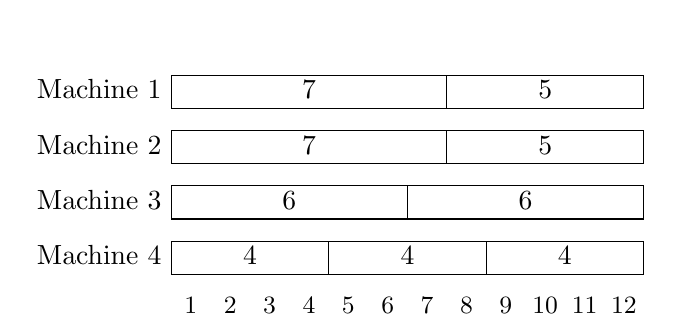
\begin{tikzpicture}[/pgfgantt/y unit chart=0.7cm] 
            \begin{ganttchart}[
                title/.style={draw=none},
                canvas/.append style={draw=none}, 
                bar top shift=0.1, bar height=0.6,
                y unit title=0.7cm,
            ]{1}{12}
                \ganttbar{Machine 1}{1}{7} \ganttbar[inline]{7}{1}{7} \ganttbar[inline]{5}{8}{12} \\ 
                \ganttbar{Machine 2}{1}{7} \ganttbar[inline]{7}{1}{7} \ganttbar[inline]{5}{8}{12} \\ 
                \ganttbar{Machine 3}{1}{6} \ganttbar[inline]{6}{1}{6} \ganttbar[inline]{6}{7}{12} \\ 
                \ganttbar{Machine 4}{1}{4} \ganttbar[inline]{4}{1}{4} \ganttbar[inline]{4}{5}{8} \ganttbar[inline]{4}{9}{12} \\
                \gantttitlelist{1,...,12}{1}
            \end{ganttchart}
        \end{tikzpicture}
    \end{center}
    \vspace{-0.4cm}
    On the other hand, LPT gives the following schedule which has $C_{\max} = 15$, 
    which is the worst case we could possibly have from Theorem~\ref{theo:6.6}.
    \begin{center} 
        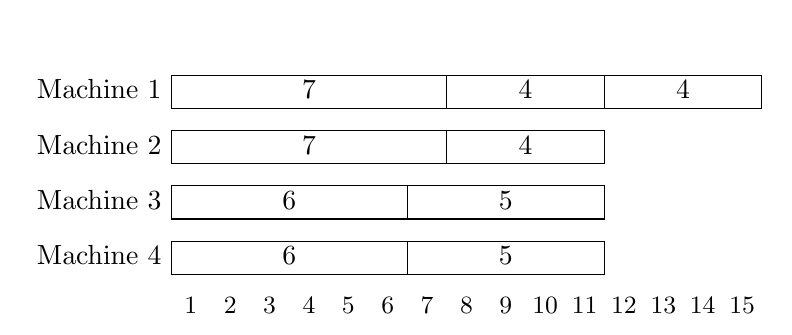
\begin{tikzpicture}[/pgfgantt/y unit chart=0.7cm] 
            \begin{ganttchart}[
                title/.style={draw=none},
                canvas/.append style={draw=none}, 
                bar top shift=0.1, bar height=0.6,
                y unit title=0.7cm,
            ]{1}{12}
                \ganttbar{Machine 1}{1}{7} \ganttbar[inline]{7}{1}{7} \ganttbar[inline]{4}{8}{11} \ganttbar[inline]{4}{12}{15} \\ 
                \ganttbar{Machine 2}{1}{7} \ganttbar[inline]{7}{1}{7} \ganttbar[inline]{4}{8}{11} \\ 
                \ganttbar{Machine 3}{1}{6} \ganttbar[inline]{6}{1}{6} \ganttbar[inline]{5}{7}{11} \\ 
                \ganttbar{Machine 4}{1}{6} \ganttbar[inline]{6}{1}{6} \ganttbar[inline]{5}{7}{11} \\
                \gantttitlelist{1,...,15}{1}
            \end{ganttchart}
        \end{tikzpicture}
    \end{center}
    \vspace{-0.4cm}
\end{exmp}

\subsubsection{Makespan with Precedence Constraints} \label{subsubsec:6.1.2}
Now, consider the same problem with the jobs subject to precedence constraints,
namely $(P_m~|~\text{prec}~|~C_{\max})$. From a complexity point of view, this 
problem has to be at least as hard as the problem without precedence constraints.
In particular, it can be shown that $(P_m~|~\text{prec}~|~C_{\max})$ is 
strongly $\NP$-hard for $2 \leq m < n$, even in the case where the precedence 
constraints are chains. To obtain some insight into the effects of precedence 
constraints, we consider a number of special cases. 

Suppose there are an unlimited number of machines in parallel, or that 
$m \geq n$ so the number of machines is at least as large as the number of jobs.
We can denote this problem by $(P_\infty~|~\text{prec}~|~C_{\max})$. This 
is a classical problem in the field of project planning, and its study 
has led to the development of the well-known {\bf Critical Path Method 
(CPM)} and {\bf Project Evaluation Review Technique (PERT)}. In this case, 
the optimal schedule and the minimum makespan are determined by a very simple 
algorithm. 

\begin{algo}[Minimizing the Makespan of a Project]{algo:6.8}
    Schedule the jobs one at a time starting at time zero. Whenever a job has 
    been completed, start all jobs of in which all predecessors have been 
    completed (that is, the set of all schedulable jobs).
\end{algo}

So $(1~|~\text{prec}~|~C_{\max})$ and $(P_\infty~|~\text{prec}~|~C_{\max})$,
are easy. But we stated earlier that $(P_m~|~\text{prec}~|~C_{\max})$ is 
strongly $\NP$-hard for $2 \leq m < n$. Even $(P_m~|~p_j = 1, \text{prec}~|~C_{\max})$,
where the processing times are all unit, is not easy. However, by constraining 
the problem further and assuming that the precedence graph takes the form 
of a tree (either an intree or an outtree), the problem $(P_m~|~p_j = 1, 
\text{tree}~|~C_{\max})$ is easily solvable. This leads to the well-known 
scheduling rule known as the {\bf Critical Path (CP)} rule. 

\begin{algo}[Critical Path (CP)]{algo:6.9}
    The job at the head of the longest string of jobs in the precedence
    constraints graph has the highest priority. Ties can be broken arbitrarily.
\end{algo}

We also consider a different priority rule that considers the largest 
total number of successors (not just the immediate successors) in the 
precedence graph. This is called the {\bf Largest Number of Successors first 
(LNS)} rule. 

\begin{algo}[Largest Number of Successors first (LNS)]{algo:6.10}
    The job with the largest total number of successors in the 
    precedence graph has the highest priority. Ties can be broken arbitrarily.
\end{algo}

Note that the LNS rule is equivalent to the CP rule when the precedence 
graph takes the form of chains or an intree. It can also be shown that 
LNS is optimal for outtrees, and thus LNS is also optimal for 
$(P_m~|~p_j = 1, \text{tree}~|~C_{\max})$.

We will not prove the optimality of the CP and LNS rules for 
$(P_m~|~p_j = 1, \text{tree}~|~C_{\max})$. But how do these rules perform for 
arbitrary precedence constraints when all processing times are equal to $1$? 

In the case where there are two parallel machines, it can be shown that 
\[ \frac{C_{\max}(\text{CP})}{C_{\max}(\text{OPT})} \leq \frac43. \] 
When there are more than two parallel machines, the worst case ratio is larger. 
We show that the worst case bound can be reached for two machines in the 
following example. 

\begin{exmp}{exmp:6.11}
    Consider the instance of $(P_2~|~p_j=1, \text{prec}~|~C_{\max})$ 
    with precedence constraints given by the following directed acyclic 
    graph. 
    \begin{center}
        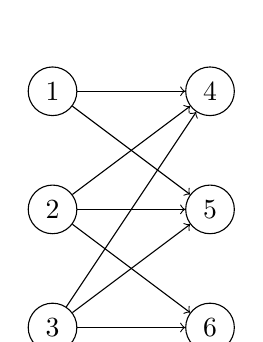
\begin{tikzpicture}              
            \node [circle, draw=black] (1) at (0, 3) {$1$};  
            \node [circle, draw=black] (2) at (0, 1.5) {$2$}; 
            \node [circle, draw=black] (3) at (0, 0) {$3$}; 
            \node [circle, draw=black] (4) at (2, 3) {$4$}; 
            \node [circle, draw=black] (5) at (2, 1.5) {$5$}; 
            \node [circle, draw=black] (6) at (2, 0) {$6$};

            \draw [->] (1) -- (4); \draw [->] (1) -- (5); 
            \draw [->] (2) -- (4); \draw [->] (2) -- (5); \draw [->] (2) -- (6);
            \draw [->] (3) -- (4); \draw [->] (3) -- (5); \draw [->] (3) -- (6);        
        \end{tikzpicture} 
    \end{center}
    This is almost a complete bipartite graph; it is only missing the edge 
    from job $1$ to job $6$. An optimal schedule is given below with 
    $C_{\max} = 3$. 
    \begin{center} 
        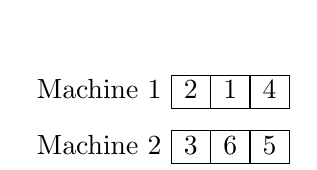
\begin{tikzpicture}[/pgfgantt/y unit chart=0.7cm] 
            \begin{ganttchart}[
                title/.style={draw=none},
                canvas/.append style={draw=none}, 
                bar top shift=0.1, bar height=0.6,
                y unit title=0.7cm,
            ]{1}{3}
                \ganttbar{Machine 1}{1}{2} \ganttbar[inline]{2}{1}{1} \ganttbar[inline]{1}{2}{2} \ganttbar[inline]{4}{3}{3} \\ 
                \ganttbar{Machine 2}{1}{2} \ganttbar[inline]{3}{1}{1} \ganttbar[inline]{6}{2}{2} \ganttbar[inline]{5}{3}{3}
            \end{ganttchart}
        \end{tikzpicture}
    \end{center}
    \vspace{-0.4cm}
    On the other hand, the CP rule could arbitrarily pick job $1$ to 
    be processed at time $0$, which would prevent job $6$ from running 
    at time $1$ as its predecessors are jobs $2$ and $3$. One such schedule 
    obtained from the CP rule is as follows, and it has $C_{\max} = 4$, 
    which matches the worst case bound above. 
    \begin{center} 
        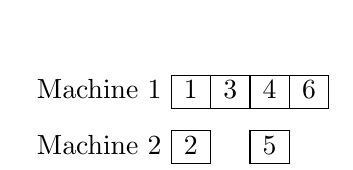
\begin{tikzpicture}[/pgfgantt/y unit chart=0.7cm] 
            \begin{ganttchart}[
                title/.style={draw=none},
                canvas/.append style={draw=none}, 
                bar top shift=0.1, bar height=0.6,
                y unit title=0.7cm,
            ]{1}{3}
                \ganttbar{Machine 1}{1}{1} \ganttbar[inline]{1}{1}{1} \ganttbar[inline]{3}{2}{2} \ganttbar[inline]{4}{3}{3} \ganttbar[inline]{6}{4}{4} \\ 
                \ganttbar{Machine 2}{1}{1} \ganttbar[inline]{2}{1}{1} \ganttbar[inline]{5}{3}{3} 
            \end{ganttchart}
        \end{tikzpicture}
    \end{center}
\end{exmp}

Next, we give an example where LNS does not yield an optimal schedule for 
arbitrary precedence constraints. 

\begin{exmp}{exmp:6.12}
    Consider the instance of $(P_2~|~p_j=1, \text{prec}~|~C_{\max})$ 
    with precedence constraints given by the following directed acyclic 
    graph. 
    \begin{center}
        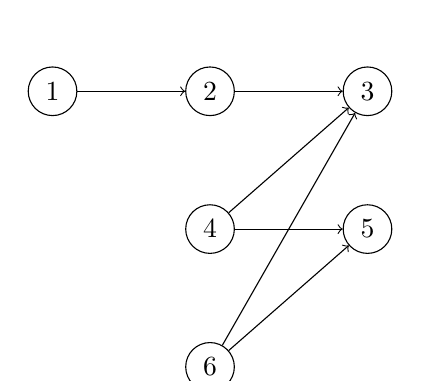
\begin{tikzpicture}              
            \node [circle, draw=black] (1) at (0, 3.5) {$1$};  
            \node [circle, draw=black] (2) at (2, 3.5) {$2$}; 
            \node [circle, draw=black] (3) at (4, 3.5) {$3$}; 
            \node [circle, draw=black] (4) at (2, 1.75) {$4$}; 
            \node [circle, draw=black] (5) at (4, 1.75) {$5$}; 
            \node [circle, draw=black] (6) at (2, 0) {$6$};

            \draw [->] (1) -- (2); \draw [->] (2) -- (3); 
            \draw [->] (4) -- (3); \draw [->] (4) -- (5);
            \draw [->] (6) -- (3); \draw [->] (6) -- (5);     
        \end{tikzpicture} 
    \end{center}
    \newpage
    An optimal schedule is given below with $C_{\max} = 3$. 
    \begin{center} 
        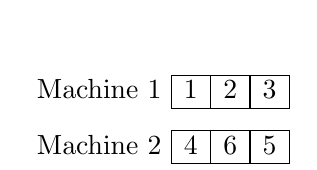
\begin{tikzpicture}[/pgfgantt/y unit chart=0.7cm] 
            \begin{ganttchart}[
                title/.style={draw=none},
                canvas/.append style={draw=none}, 
                bar top shift=0.1, bar height=0.6,
                y unit title=0.7cm,
            ]{1}{3}
                \ganttbar{Machine 1}{1}{2} \ganttbar[inline]{1}{1}{1} \ganttbar[inline]{2}{2}{2} \ganttbar[inline]{3}{3}{3} \\ 
                \ganttbar{Machine 2}{1}{2} \ganttbar[inline]{4}{1}{1} \ganttbar[inline]{6}{2}{2} \ganttbar[inline]{5}{3}{3}
            \end{ganttchart}
        \end{tikzpicture}
    \end{center}
    \vspace{-0.4cm}
    The LNS rule would pick jobs $4$ and $6$ first as they each have two 
    successors. This causes job $2$ to finish at time $3$ at the earliest, 
    preventing job $3$ from being run afterwards. So the LNS rule 
    yields a schedule with $C_{\max} = 4$. 
    \begin{center} 
        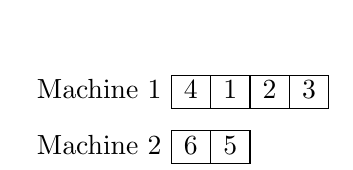
\begin{tikzpicture}[/pgfgantt/y unit chart=0.7cm] 
            \begin{ganttchart}[
                title/.style={draw=none},
                canvas/.append style={draw=none}, 
                bar top shift=0.1, bar height=0.6,
                y unit title=0.7cm,
            ]{1}{3}
                \ganttbar{Machine 1}{1}{2} \ganttbar[inline]{4}{1}{1} \ganttbar[inline]{1}{2}{2} \ganttbar[inline]{2}{3}{3} \ganttbar[inline]{3}{4}{4} \\ 
                \ganttbar{Machine 2}{1}{2} \ganttbar[inline]{6}{1}{1} \ganttbar[inline]{5}{2}{2} 
            \end{ganttchart}
        \end{tikzpicture}
    \end{center}
    \vspace{-0.4cm}
\end{exmp}

Both the CP rule and the LNS rule have more generalized versions that
can be applied to problems with arbitrary job processing times. Instead of
counting the number of jobs (as in the case with unit processing times), these
more generalized versions prioritize based on the total amount of processing
remaining to be done on the jobs in question. The CP rule then gives the
highest priority to the job that is heading the string of jobs with the largest
total amount of processing (with the processing time of the job itself also being
included in this total). The generalization of the LNS rule gives the highest
priority to that job that precedes the largest total amount of processing; again
the processing time of the job itself is also included in the total. The LNS name
is clearly not appropriate for this generalization with arbitrary processing times,
as it refers to a number of jobs rather than to a total amount of processing.

\subsubsection{Makespan with Machine Dependent Constraints} \label{subsubsec:6.1.3}
We consider another generalization of the $(P_m~||~C_{\max})$ problem 
where each job $j$ is only allowed to be run on a subset $M_j$ of the $m$ 
parallel machines. We will again consider the case with unit processing times, 
denoted by $(P_m~|~p_j=1, M_j~|~C_{\max})$. 

We note that this problem can be represented using a bipartite graph with $n$ 
edges $1, \dots, n$ corresponding to the jobs and $m$ edges $\text{mc}_1, 
\dots, \text{mc}_m$ corresponding to the machines. We place an edge 
$(j, \text{mc}_i)$ in the graph if and only if $i \in M_j$. 

We say that the sets $M_j$ are {\bf nested} if exactly one of the 
following conditions hold for any two jobs $j$ and $k$: 
\begin{enumerate}[(i)]
    \item $M_j = M_k$; 
    \item $M_j \subsetneq M_k$;
    \item $M_k \subsetneq M_j$; or 
    \item $M_j \cap M_k = \varnothing$.
\end{enumerate} 
When the sets $M_j$ are nested, the {\bf Least Flexible Job (LFJ)} rule 
plays an important role. 

\begin{algo}[Least Flexible Job (LFJ)]{algo:6.13}
    Every time a machine is freed, select among the available jobs the job 
    that can be processed on the \emph{smallest} number of machines. Ties 
    can be broken arbitrarily. 
\end{algo}

This rule is rather crude as it does not specify, for example, which
machine should be considered first when several machines become available at
the same time. It can be shown that the LFJ rule is optimal for 
$(P_m~|~p_j=1, M_j~|~C_{\max})$ when the sets $M_j$ are nested by using 
a standard interchange argument. In particular, when there are two 
machines, the sets $M_j$ are always nested, so the LFJ rule is optimal 
for $(P_2~|~p_j=1, M_j~|~C_{\max})$. However, in the case that $m \geq 3$ 
and the sets $M_j$ are arbitrary, the LFJ rule will not always yield an 
optimal schedule. We give an example of this below. 

\begin{exmp}{exmp:6.14}
    Consider the following instance of $(P_4~|~p_j=1, M_j~|~C_{\max})$ 
    with $n = 8$ jobs. 
    \begin{align*}
        \begin{array}{c|cccccccc}
            j & 1 & 2 & 3 & 4 & 5 & 6 & 7 & 8 \\ \hline 
            M_j & \{1,2\} & \{1,3,4\} & \{1,3,4\} & \{2\} & \{3,4\} 
            & \{3,4\} & \{3,4\} & \{3,4\}
        \end{array}
    \end{align*}
    It is clear that the sets $M_j$ are not nested by considering $M_1$ 
    and $M_2$. We now run the LFJ rule. Consider machine $1$ first. 
    The least flexible job that can be processed on machine $1$ is job $1$ 
    since it can be processed on only two machines, while jobs $2$ and $3$ 
    can be processed on three machines. The least flexible job to be processed 
    on machine $2$ is clearly job $4$. At time $0$, the least flexible jobs 
    to be processed on machines $3$ and $4$ could be jobs $5$ and $6$. 
    At time $1$, after jobs $1$, $4$, $5$, and $6$ have completed their processing 
    on the four machines, the least flexible job to be processed on machine 
    $1$ is job $2$. But none of the remaining jobs can be processed on 
    machine $2$, so it is forced to idle. The least flexible jobs to 
    go on machines $3$ and $4$ are jobs $7$ and $8$. Finally, job $3$ 
    can be run on machine $1$ at time $3$, so $C_{\max} = 3$. This schedule 
    is illustrated below. 
    \begin{center} 
        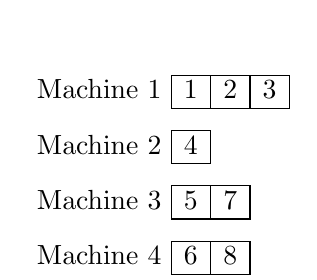
\begin{tikzpicture}[/pgfgantt/y unit chart=0.7cm] 
            \begin{ganttchart}[
                title/.style={draw=none},
                canvas/.append style={draw=none}, 
                bar top shift=0.1, bar height=0.6,
                y unit title=0.7cm,
            ]{1}{3}
                \ganttbar{Machine 1}{1}{1} \ganttbar[inline]{1}{1}{1} \ganttbar[inline]{2}{2}{2} \ganttbar[inline]{3}{3}{3} \\
                \ganttbar{Machine 2}{1}{1} \ganttbar[inline]{4}{1}{1} \\
                \ganttbar{Machine 3}{1}{1} \ganttbar[inline]{5}{1}{1} \ganttbar[inline]{7}{2}{2} \\ 
                \ganttbar{Machine 4}{1}{1} \ganttbar[inline]{6}{1}{1} \ganttbar[inline]{8}{2}{2}
            \end{ganttchart}
        \end{tikzpicture}
    \end{center}
    \vspace{-0.4cm}
    An optimal schedule with $C_{\max} = 2$ is given below, so LFJ was not optimal. 
    \begin{center} 
        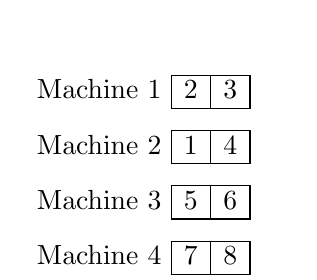
\begin{tikzpicture}[/pgfgantt/y unit chart=0.7cm] 
            \begin{ganttchart}[
                title/.style={draw=none},
                canvas/.append style={draw=none}, 
                bar top shift=0.1, bar height=0.6,
                y unit title=0.7cm,
            ]{1}{3}
                \ganttbar{Machine 1}{1}{1} \ganttbar[inline]{2}{1}{1} \ganttbar[inline]{3}{2}{2} \\
                \ganttbar{Machine 2}{1}{1} \ganttbar[inline]{1}{1}{1} \ganttbar[inline]{4}{2}{2} \\
                \ganttbar{Machine 3}{1}{1} \ganttbar[inline]{5}{1}{1} \ganttbar[inline]{6}{2}{2} \\ 
                \ganttbar{Machine 4}{1}{1} \ganttbar[inline]{7}{1}{1} \ganttbar[inline]{8}{2}{2}
            \end{ganttchart}
        \end{tikzpicture}
    \end{center}
\end{exmp}

From Example~\ref{exmp:6.14}, one may expect that if a number of machines are 
free at the same point in time, it is advantageous to consider first the least 
flexible machine. The flexibility of a machine could be defined as the number 
of remaining jobs that can be processed (or the total amount of processing that 
can be done) on that machine. However, assigning any job to the {\bf Least 
Flexible Machine (LFM)} at each point in time does not guarantee an optimal
schedule in the case of Example~\ref{exmp:6.14}.

Heuristics can be designed that combine the LFJ rule with the LFM rule,
giving priority to the least flexible jobs on the least flexible machines. That is,
consider at each point in time first the Least Flexible Machine (LFM) (that is,
the machine that can process the smallest number of jobs) and assign to this
machine the least flexible job that can be processed on it. Any ties may be
broken arbitrarily. This heuristic may be referred to as the LFM-LFJ heuristic.
However, we find again that the LFM-LFJ does not yield an optimal schedule for 
Example~\ref{exmp:6.14}.

\subsection{Makespan with Preemptions} \label{subsec:6.2}
We now consider the same problem with preemptions allowed, namely the 
$(P_m~|~\text{prmp}~|~C_{\max})$ problem. Usually, but not always, allowing 
preemptions simplifies the analysis of a problem. This is indeed the case for 
this problem, where it actually turns out that many schedules are optimal. 
First, consider the following linear programming formulation of the problem, 
where $x_{ij}$ is the total time spent by machine $i$ on job $j$. 
\begin{align*}
    \min\quad & C_{\max} \\ 
    \text{s.t.}\quad & \sum_{i=1}^m x_{ij} = p_j, && j \in [n] \\ 
    & \sum_{i=1}^m x_{ij} \leq C_{\max}, && j \in [n] \\
    & \sum_{j=1}^n x_{ij} \leq C_{\max}, && i \in [m] \\
    & x_{ij} \geq 0, && i \in [m],\,j \in [n]. 
\end{align*}
The first set of constraints ensures that each job receives the required 
amount of processing. The second set of constraints ensures that the total 
amount of processing of each job is less than the makespan. The third 
set of constraints ensures that the total amount of processing on each 
machine is less than the makespan. Finally, the last constraint ensures that 
the execution fragments are non-negative. 

Since $C_{\max}$ is basically a decision variable and not an element of 
the resource vector of the linear program, we can rewrite the second and third 
set of constraints as 
\begin{align*}
    C_{\max} - \sum_{i=1}^m x_{ij} &\geq 0, && j \in [n] \\ 
    C_{\max} - \sum_{j=1}^n x_{ij} &\geq 0, && i \in [m]. 
\end{align*}
This LP can be solved in polynomial time, but the solution of the LP does
not prescribe an actual schedule; it merely specifies the amount of time job
$j$ should spend on machine $i$. However, with this information, a schedule can
easily be constructed.

We consider another algorithm for $(P_m~|~\text{prmp}~|~C_{\max})$. This 
algorithm is based on the fact that it is easy to obtain an expression for the
makespan under the optimal schedule. In the next lemma, we establish a lower 
bound. We leave its proof as an exercise. 

\begin{lemma}{lemma:6.15}
    Under the optimal schedule for $(P_m~|~\text{prmp}~|~C_{\max})$, we have 
    \[ C_{\max} \geq \max\left( p_1, \frac1m \sum_{j=1}^n p_j \right) 
    =: C^*_{\max}. \] 
\end{lemma}

Having a lower bound allows for the construction of a very simple algorithm
that minimizes the makespan. The fact that this algorithm actually produces
a schedule with a makespan that is equal to the lower bound shows that the
algorithm yields an optimal schedule. This algorithm is also known 
as {\bf McNaughton's wrap-around rule}. 

\begin{algo}[Minimizing Makespan with Preemptions]{algo:6.16}
    \begin{enumerate}
        \item Take the $n$ jobs and process them one after another on a single 
        machine in any sequence (that is, without preemption). The makespan is 
        then equal to the sum of the $n$ processing times and is at most 
        $m \cdot C^*_{\max}$.
        
        \item Take this single machine schedule and divide it into $m$ equal parts.
        
        \item Execute each of the $m$ parts in Step 2 on a separate machine. 
    \end{enumerate}
\end{algo}

It is clear that the resulting schedule is feasible. Part of a job may appear
at the end of the schedule for machine $i$ while the remaining part may appear
at the beginning of the schedule for machine $i + 1$. As preemptions are allowed
and the processing time of each job is less than $C^*_{\max}$, such a schedule 
is feasible. Moreover, this schedule has $C_{\max} = C^*_{\max}$, so it is 
also optimal. 

Next, we consider the {\bf Longest Remaining Processing Time first (LRPT)} 
rule. This schedule is the preemptive version of LPT (Algorithm~\ref{algo:6.3}).
This schedule is structurally appealing, but it is mainly of academic interest. 
From a practical point, it has a serious drawback. In the deterministic case, 
the number of preemptions needed is usually infinite. 

\begin{exmp}{exmp:6.17}
    Consider two jobs with unit processing time on a single machine. 
    Under LRPT, the two jobs continuously have to rotate and wait for their 
    next turn on the machine. That is, a job stays on the machine for a 
    time period $\eps$ and after every time period $\eps$, the job 
    waiting preempts the machine. The makespan is equal to $2$, and is 
    independent of the schedule. However, the sum of completion times is 
    $4 - \eps$, while under the non-preemptive schedule, it is $3$. 
    This suggests that LRPT is a bad rule for $(P_m~|~\text{prmp}~|~\sum C_j)$, 
    but we are not interested in this problem at the moment. 
\end{exmp}

We will now assume that we are working under a discrete time framework. 
All processing times are assumed to be integer, and the decision-maker 
is only allowed to preempt a machine at integer times. 
The following is an example of the LRPT rule under discrete time. 

\begin{exmp}{exmp:6.18}
    Suppose there are two machines, and three jobs $1, 2, 3$ with processing 
    times $8, 7, 6$ respectively. Then the schedule under LRPT is depicted 
    below and has makespan $11$. 
    \begin{center} 
        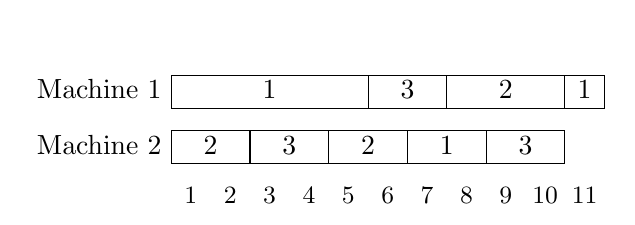
\begin{tikzpicture}[/pgfgantt/y unit chart=0.7cm] 
            \begin{ganttchart}[
                title/.style={draw=none},
                canvas/.append style={draw=none}, 
                bar top shift=0.1, bar height=0.6,
                y unit title=0.7cm,
            ]{1}{11}
                \ganttbar{Machine 1}{1}{5} \ganttbar[inline]{1}{1}{5} \ganttbar[inline]{3}{6}{7} \ganttbar[inline]{2}{8}{10} \ganttbar[inline]{1}{11}{11} \\
                \ganttbar{Machine 2}{1}{2} \ganttbar[inline]{2}{1}{2} \ganttbar[inline]{3}{3}{4} \ganttbar[inline]{2}{5}{6} \ganttbar[inline]{1}{7}{8} \ganttbar[inline]{3}{9}{10} \\
                \gantttitlelist{1,...,11}{1}
            \end{ganttchart}
        \end{tikzpicture}
    \end{center}
\end{exmp}

To prove that LRPT is optimal for $(P_m~|~\text{prmp}~|~C_{\max})$ under 
discrete time, we require some special notation. 

Suppose that at integer time $t$, the remaining processing times of the 
$n$ jobs are $p_1(t), \dots, p_n(t)$. We let $\overline p(t) = 
(p_1(t), \dots, p_n(t))$ be the vector of processing times. Let 
$p_{(j)}$ denote the $j$-th largest element of $\overline p(t)$. We say that 
$\overline p(t)$ {\bf majorizes} $\overline q(t)$, written $\overline p(t) \geq_m 
\overline q(t)$, if for all $1 \leq k \leq n$, we have 
\[ \sum_{j=1}^k p_{(j)}(t) \geq \sum_{j=1}^k q_{(j)}(t). \] 

\begin{exmp}{exmp:6.19}
    Consider the vectors $\overline p(t) = (4, 8, 2, 4)$ and $\overline q(t) = 
    (3, 0, 6, 6)$. Placing the elements of the vectors in decreasing order 
    yields $(8, 4, 4, 2)$ and $(6, 6, 3, 0)$, and it is easily seen that 
    $\overline p(t) \geq_m \overline q(t)$. 
\end{exmp}

\begin{lemma}{lemma:6.20}
    If $\overline p(t) \geq_m \overline q(t)$, then LRPT applied to 
    $\overline p(t)$ results in a makespan that is greater or equal to 
    the makespan obtained from applying LRPT to $\overline q(t)$. 
\end{lemma}
\begin{pf}
    We proceed by induction on the \emph{total} amount of remaining processing.
    To show that the lemma holds for $\overline p(t)$ and $\overline q(t)$ 
    with total processing time $\sum_{j=1}^n p_j(t)$ and $\sum_{j=1}^n q_j(t)$ 
    respectively, we assume that the result holds for all pairs of vectors 
    with total remaining processing time at most $\sum_{j=1}^n p_j(t) - 1$ 
    and $\sum_{j=1}^n q_j(t) - 1$, respectively. The base case can be 
    easily checked by considering the two vectors $(1, 0, \dots, 0)$ and 
    $(1, 0, \dots, 0)$. 

    If LRPT is applied for one time unit on $\overline p(t)$ and $\overline q(t)$ 
    respectively, then the vectors of remaining processing times at time 
    $t+1$ are $\overline p(t+1)$ and $\overline q(t+1)$ respectively. It is 
    clear that 
    \begin{align*}
        \sum_{j=1}^n p_{(j)}(t+1) &\leq \sum_{j=1}^n p_{(j)}(t) - 1, \\ 
        \sum_{j=1}^n q_{(j)}(t+1) &\leq \sum_{j=1}^n q_{(j)}(t) - 1.
    \end{align*}
    It can be shown that if $\overline p(t) \geq_m \overline q(t)$, then 
    $\overline p(t+1) \geq_m \overline q(t+1)$. Notice that LRPT results in a 
    larger makespan at time $t + 1$ due to the induction hypothesis, 
    and so it also results in a larger makespan at time $t$. 

    If there are fewer than $m$ jobs remaining to be processed, then 
    it is clear that the lemma holds. 
\end{pf}

\begin{theo}{theo:6.21}
    LRPT is optimal for $(P_m~|~\text{prmp}~|~C_{\max})$ in discrete time. 
\end{theo}
\begin{pf}
    The first step of the induction is shown as follows. Suppose no more than
    $m$ jobs have processing times remaining and that these jobs all have only 
    one unit of processing time left. Then clearly LRPT is optimal in this case.

    Assume that LRPT is optimal for any vector $\overline p(t)$ such that 
    \[ \sum_{j=1}^n p_{(j)}(t) \leq N-1. \] 
    Now, consider a vector $\overline p(t)$ with 
    \[ \sum_{j=1}^n p_{(j)}(t) = N. \] 
    We again proceed by induction on the total amount of remaining processing.
    Here, we assume towards a contradiction that LRPT is not optimal 
    for $\overline p(t)$. Since LRPT is not optimal, then there must be 
    some other rule, say R, that is optimal. Note that R does not act according to 
    LRPT at time $t$, but from time $t + 1$ onwards, it must act according to 
    LRPT due to the induction hypothesis. We compare applying LRPT at time 
    $t$ to $\overline p(t)$ as opposed to applying R at time $t$ to 
    the same vector $\overline p(t)$. Let $\overline p(t+1)$ and 
    $\overline p'(t+1)$ denote the vectors of remaining processing times 
    at time $t+1$ after applying LRPT and R. It is clear that 
    $\overline p'(t+1) \geq_m \overline p(t+1)$. From Lemma~\ref{lemma:6.20}, 
    it follows that the makespan under R is larger than the makespan under 
    LRPT. This is a contradiction, which completes the proof. 
\end{pf}

Notice that when we multiply all processing times by a large integer $K$,
the problem intrinsically does not change, as the relative lengths of the 
processing times remains the same. The optimal policy is again LRPT. But now, 
there are many more preemptions (at integral time units). Multiplying all 
processing times by $K$ has the effect that the time slots become smaller 
relative to the processing times and the decision maker is allowed to preempt 
after shorter intervals. Letting $K \to \infty$ shows that LRPT is optimal in 
continuous time as well. 

\subsection{Dynamic Programming and PTAS for Makespan} \label{subsec:6.3}
We now return to the $\NP$-hard problem $(P~||~C_{\max})$, where the 
number of machines is \emph{not} fixed. We first focus on a special 
case where the processing times $p_j$ take on $k$ distinct values. We use 
dynamic programming algorithm to solve this special case in $n^{O(k)}$ time. 
Assume that we are given a target schedule length $T$.

Suppose that the $k$ distinct values are $b_1, \dots, b_k$. Let $n_i = 
|\{j \in [n] : p_j = b_i\}|$ be the total number of jobs with processing 
time $b_i$. The key observation is that a subset of jobs can be described with a 
$k$-dimensional vector $\mathbf x = (x_1, \dots, x_k)$ where $x_i$ is the number 
of jobs of processing time $b_i$. 

We define $M(\mathbf x)$ to be the minimum number of machines needed 
to schedule all jobs in $\mathbf x$ with makespan $\leq T$. Next, we define 
$Q$ to be the set of vectors $\mathbf a = (a_1, \dots, a_k)$ that can be 
scheduled on {\bf one} machine with makespan $\leq T$. That is, we have 
\[ Q = \left\{ \mathbf a = (a_1, \dots, a_k) : \sum_{i=1}^k a_i b_i \leq T \right\}. \] 
We will exclude the zero vector $\mathbf 0$ from $Q$, as it is not useful to us.
We now state the dynamic programming algorithm for our special case.  

\begin{algo}[Dynamic programming for special case of $(P~||~C_{\max})$]{algo:6.22}
    Initially, set $M(\mathbf a) = 1$ if $\mathbf a \in Q$, and 
    set $M(\mathbf 0) = 0$. We wish to compute $M(n_1, \dots, n_k)$. 
    We can do this via a $k$-dimensional table with $n_1 \times \cdots \times 
    n_k$ entries via the recursive relation 
    \[ M(x_1, \dots, x_k) = 1 + \min\{M(x_1 - a_1, \dots, x_k - a_k) : 
    \mathbf a \in Q\}. \]  
\end{algo}

We see that there are at most $n^k$ entries in the table, and that the 
computation of each entry relies on $O(n^k)$ other entries. Therefore, 
the total computation time of Algorithm~\ref{algo:6.22} is $n^{O(k)}$. 

It remains to handle the assumption that we know the target schedule length $T$. 
The easiest way to do this is to perform a binary search on all possible values 
of $T$. We will go into more detail on this later when we discuss the PTAS 
for the more general case of this problem. 

\begin{exmp}{exmp:6.23}
    Suppose there are two distinct values of jobs, namely $b_1 = 1$ 
    and $b_2 = 10$. Moreover, suppose that $n_1 = n_2 = 5$, and 
    our target schedule length is $T = 12$. First, observe that 
    \[ Q = \{(1, 0), (2, 0), (3, 0), (4, 0), (5, 0), (0, 1), (1, 1), (2, 1)\} \] 
    is the set of schedules that have makespan $\leq 12$ on one machine. 
    Then $M(0, 0) = 0$ and $M(\mathbf a) = 1$ for all $\mathbf a \in Q$. 
    We then use the relation $M(\mathbf x) = 1 + \min\{M(\mathbf x - \mathbf a) 
    : \mathbf a \in Q\}$ to compute the rest of the table, as follows. 
    \begin{align*}
        \begin{array}{c|c|c|c|c|c|c} 
            M(x_1, x_2) & x_2 = 0 & x_2 = 1 & x_2 = 2 & x_2 = 3 & x_2 = 4 & x_2 = 5 \\ \hline 
            x_1 = 0 & 0 & 1 & 2 & 3 & 4 & 5 \\ \hline 
            x_1 = 1 & 1 & 1 & 2 & 3 & 4 & 5 \\ \hline 
            x_1 = 2 & 1 & 1 & 2 & 3 & 4 & 5 \\ \hline 
            x_1 = 3 & 1 & 2 & 2 & 3 & 4 & 5 \\ \hline 
            x_1 = 4 & 1 & 2 & 2 & 3 & 4 & 5 \\ \hline 
            x_1 = 5 & 1 & 2 & 3 & 3 & 4 & 5 
        \end{array}
    \end{align*}
\end{exmp}

We now discuss the general case $(P~||~C_{\max})$ without the assumption 
where the processing times $p_j$ take on $k$ distinct values. In this 
case, we will focus mainly on the larger jobs. We will round and scale 
these jobs so that there is at most a constant number of sizes of large 
jobs, and apply the dynamic programming algorithm (Algorithm~\ref{algo:6.22}) 
to these rounded jobs. We then finish up by scheduling the small jobs greedily 
via the list scheduling algorithm (Algorithm~\ref{algo:6.1}).

We consider a {\bf relaxed decision procedure (RDP)} for the problem, 
which takes as inputs an error parameter $\eps > 0$ and a target makespan $T$. 
It returns ``no'' if the optimal makespan is $>T$, and returns ``yes'' 
if the optimal makespan is $\leq (1+\eps)T$ along with such a schedule. 
Using this RDP, we obtain a $(1+\eps)$-approximation algorithm for 
$(P~||~C_{\max})$, which also takes $\eps > 0$ and $T$ as input. 

\begin{algo}[PTAS for $(P~||~C_{\max})$]{algo:6.24}
    \begin{enumerate}[(1)]
        \item Partition the jobs into small jobs $\{j : p_j \leq \eps T\}$ 
        and large jobs $\{j : p_j > \eps T\}$. 
        \item Call the RDP on the large jobs. Note that this can be done 
        by running the dynamic programming algorithm (Algorithm~\ref{algo:6.22}) 
        after we perform rounding and scaling to the large jobs. 
        \item If the RDP returns ``no'', then output ``no schedule of 
        length $\leq T$ exists''. If the RDP returns ``yes'' and a schedule 
        $\hat S$, apply list scheduling (Algorithm~\ref{algo:6.1}) to place 
        the small jobs into $\hat S$. Call this schedule $S^\text{new}$. 
        \item If the makespan of $S^{\text{new}}$ is $>(1+\eps)T$, then 
        output ``no schedule of length $\leq T$ exists''. Otherwise, 
        return ``yes'' and the schedule $S^\text{new}$. 
    \end{enumerate}
\end{algo}

Note that this algorithm can terminate at three points: Step 3 when the 
RDP returns ``no'', and Step 4 depending on the makespan of $S^{\text{new}}$. 
To prove correctness, it suffices to consider when the makespan of 
$S^{\text{new}}$ is $>(1+\eps)T$; it is clear that the other outputs are correct. 
Note that the last job to complete in $S^{\text{new}}$ must be a small job, 
because if the last job were a large job, then the algorithm would have terminated 
at Step 3. Call this last job $\ell$, and note that $C_\ell > (1+\eps)T$ 
by assumption. Then the starting time of job $\ell$ is $S_\ell \geq 
C_\ell - \eps T > T$, meaning that all machines are busy at time $S_\ell$. 
Then the optimal makespan is $\geq S_\ell > T$, so the output is correct. 

We now say a few words on how we can obtain the target makespan $T$. 
Let $\alpha = \max(p_{\max}, \frac1m \sum_{j=1}^n p_j)$. One can argue 
similar to Lemma~\ref{lemma:6.15} that $\alpha$ is a lower bound on the 
optimal makespan OPT for $(P~||~C_{\max})$. This tells us that 
\[ \alpha - 1 < \text{OPT} < 2\alpha, \] 
where the upper bound is obtained by our list scheduling result, namely 
Theorem~\ref{theo:6.2}. This means that we can start with the search 
space $(\alpha - 1, 2\alpha)$, and fix $T = \frac32\alpha$. Given 
$\eps > 0$, set $\hat \eps = \eps/3$. Then, call RDP with inputs 
$\hat \eps$ and $T$. If the output is ``no'', then we know that 
$\text{OPT} \in (\frac32\alpha, 2\alpha)$. On the other hand, if the 
output is ``yes'', we obtain a schedule with makespan $\leq (1 + 
\hat \eps) \frac32\alpha$. We can continue this binary search until the 
length of the search interval is $\leq \hat\eps \alpha$. 

\subsection{Total Completion Time without Preemptions} \label{subsec:6.4}
Consider $m$ machines in parallel and $n$ jobs. Assume that the 
jobs are ordered such that $p_1 \geq \cdots \geq p_n$. Recall from 
Theorem~\ref{theo:2.2} that the SPT rule is optimal for $(1~||~\sum C_j)$. 
This result can be proved in a different way fairly easily. 

Let $p_{(j)}$ denote the processing time of the job in the $j$-th position 
in the sequence. Then the total completion time is can be expressed as 
\[ \sum C_j = np_{(1)} + (n-1)p_{(2)} + \cdots + 2p_{(n-1)} + p_{(n)}. \] 
There are $n$ coefficients $n, n-1, \dots, 1$ to be assigned to 
$n$ different processing times. In order to minimize the above sum, 
it follows that the smallest processing time $p_n$ should be assigned to 
the largest coefficient $n$, the second smallest processing time $p_{n-1}$ 
should be assigned to the second largest coefficient $n-1$, and so on.
This implies that SPT is optimal. We can extend this type of argument 
to the parallel machine setting. 

\begin{theo}{theo:6.25}
    The SPT rule is optimal for $(P_m~||~\sum C_j)$. 
\end{theo}
\begin{pf}
    In the case of parallel machines, there are $nm$ coefficients that
    processing times can be assigned to. In particular, there are $m$ 
    copies of each of $n, n-1, \dots, 1$. The processing times have to be 
    assigned to a subset of these coefficients in order to minimize the sum of 
    the products. 

    We may assume without loss of generality that $n/m$ is an integer 
    because if not, then we can add a number of dummy jobs of processing time 
    $0$. This does not change the problem because these jobs can be 
    instantaneously processed at time $0$ and would not contribute to the 
    objective function. 

    In a similar manner to above, we see that the set of $m$ longest processing 
    times have to be assigned to the $m$ copies of $1$, and so on until the 
    $m$ shortest processing times are assigned to the $m$ copies of $n$. 
    We claim that this class of schedules includes SPT. According to the 
    SPT rule, the smallest job has to go on machine $1$ at time $0$, the 
    second smallest job goes on machine $2$ at time $0$, and so on. Next, 
    the $(m+1)$-th smallest job follows the smallest job on machine $1$, 
    the $(m+2)$-th smallest job follows the second smallest job on machine $2$, 
    and so on. We see that this assignment satisfies the properties outlined 
    above, so SPT is optimal. 
\end{pf}

From the proof of Theorem~\ref{theo:6.25}, we see that the SPT is not the only 
schedule that is optimal. Many more schedules also minimize the total 
completion time. It turns out that it is fairly easy to characterize the 
class of schedules that minimizes the total completion time; we will 
show this on Assignment 8. 

Unfortunately, we cannot generalize Theorem~\ref{theo:2.3}, which states that 
the WSPT rule is optimal for $(1~||~\sum w_j C_j)$, to the parallel 
machine setting. This is shown in the following example. 

\begin{exmp}{exmp:6.26}
    Consider two machines and three jobs as below. 
    \begin{align*}
        \begin{array}{c|ccc}
            j & 1 & 2 & 3 \\ \hline 
            p_j & 1 & 1 & 3 \\ 
            w_j & 1 & 1 & 3
        \end{array}
    \end{align*}
    Scheduling jobs $1$ and $2$ at time $0$ and job $3$ at time $1$ 
    results in a total weighted completion time of $14$, while 
    scheduling job $3$ at time $0$ and jobs $1$ and $2$ on the other machine 
    yields a total weighted completion time of $12$. Note that with this 
    set of data, any schedule is WSPT. However, changing the weights of jobs 
    $1$ and $2$ to be $1 - \eps$ shows that WSPT does not 
    necessarily yield an optimal schedule. 
\end{exmp}

In the literature, it has been shown that the WSPT heuristic is nonetheless 
a good one for the total weighted completion time on parallel machines. 
A worst case analysis of this heuristic yields the bound 
\[ \frac{\sum w_j C_j(\text{WSPT})}{\sum w_j C_j(\text{OPT})} < 
\frac12 (1 + \sqrt2). \] 
We now consider the model $(R_m~||~\sum C_j)$. Recall from Section~\ref{subsec:1.2}
that the machines in the $R_m$ environment are entirely unrelated. For example, 
machine $1$ may be able to process job $1$ in a short time and may need a long 
time for job $2$, while machine $2$ may be able to process job $2$ in a 
short time while taking a long time for job $1$. Note that identical 
parallel machines where jobs $j$ are restricted to machine sets $M_j$ 
is also a special case of this. Indeed, the processing time of a job $j$ 
on a machine that is not part of $M_j$ can be considered very long, 
making it impossible to process the job on such a machine. 

We can formulate the $(R_m~||~\sum C_j)$ problem as an integer program 
with a special structure that makes it possible to solve the problem in 
polynomial time. Recall that if job $j$ is processed on machine $i$ 
and there are $k-1$ jobs following job $j$ on this machine $i$, then 
job $j$ contributes $kp_{ij}$ to the value of the objective function. 
Let $x_{ikj} = 1$ if job $j$ is scheduled as the $k$-th to last job 
on machine $i$, and $x_{ikj} = 0$ otherwise. Then the integer 
program is as follows: 
\begin{align*}
    \min\quad & \sum_{i=1}^m \sum_{j=1}^n \sum_{k=1}^n kp_{ij} x_{ikj} \\ 
    \text{s.t.}\quad & \sum_{i=1}^m \sum_{k=1}^n x_{ikj} = 1, && j \in [n] \\ 
    & \sum_{j=1}^n x_{ikj} \leq 1, && i \in [m],\; k \in [n] \\ 
    & x_{ikj} \in \{0, 1\}, && i \in [m],\; k \in [n],\; j \in [n]. 
\end{align*}
The constraints make sure that each job is scheduled exactly once, and each
position on each machine is taken by at most one job. Note that the processing
times only appear in the objective function.

This is a so-called weighted bipartite matching problem, which has 
$n$ jobs on one side and $nm$ positions on the other side (each machine can 
process at most $n$ jobs). If job $j$ is matched with (assigned to) 
position $ik$, then there is a cost $kp_{ij}$. The objective is to 
determine the matching in this bipartite graph with a minimum cost. 
It is known from the theory of network flows that the integrality constraints 
on the $x_{ikj}$ may be replaced by non-negativity constraints
without changing the feasible set.  This weighted bipartite matching problem
then reduces to a regular linear program for which there exist polynomial time
algorithms. Note that the optimal schedule does not have to be a non-delay schedule.\newpage
\section{Flow Shops} \label{sec:7}
In many cases, each job has to undergo a series of operations. 
Often, these operations have to be done on all jobs in the same
order, implying that the jobs have to follow the same route.
The machines are then assumed to be set up in series and the environment 
is referred to as a flow shop. We saw an example of this in 
Example~\ref{exmp:1.3}; other real life examples are manufacturing and 
assembly facilities. 

We will mainly consider the makespan objective. The makespan objective is of 
considerable practical interest as its minimization is to a certain extent 
equivalent to the maximization of the utilization of the
machines. The models, however, tend to be of such complexity that makespan
results are already relatively hard to obtain. Total completion time and due
date related objectives tend to be even harder.

\subsection{Permutation Flow Shops} \label{subsec:7.1}
When searching for an optimal schedule for $(F_m~||~C_{\max})$, 
a natural question to ask is whether it suffices merely to determine 
a permutation in which the jobs traverse the entire system. 
It may be possible for one job to ``pass'' another while they are 
waiting in queue for a machine that is busy. This means that the 
machines might not be operating according to the ``first come first 
served'' principle, and that the sequence in which the jobs go through the 
machines may change from one machine to another. Changing the sequence of the 
jobs waiting in a queue between two machines may at times result in a smaller 
makespan. However, it can be shown that there always exists an optimal 
schedule without job sequence changes between the first two machines 
and the last two machines. This implies that there are optimal schedules for 
$(F_2~||~C_{\max})$ and $(F_3~||~C_{\max})$ that do not require 
sequence changes between machines. There are examples of flow shops with 
four machines in which the optimal schedule does require a job sequence 
change between the second and third machine. 

Finding an optimal schedule when sequence changes are allowed is significantly
harder than finding an optimal schedule when sequence changes are not
allowed. Flow shops that do not allow sequence changes between machines are
called {\bf permutation flow shops}. In these flow shops, the same sequence, 
or permutation, of jobs is maintained throughout. We denote this 
problem by $(F_m~|~\text{prmu}~|~C_{\max})$. Many results we will
look at concern permutation flow shops. 

Given a permutation schedule $j_1, \dots, j_n$ for a flow shop with $m$ 
machines, the completion time of a job $j_k$ at machine $i$ can be 
computed through a set of recursive equations. In particular, we have 
\begin{align*}
    C_{i,j_1} &= \sum_{\ell=1}^i p_{\ell,j_1}, && i = 1, \dots, m, \\ 
    C_{1,j_k} &= \sum_{\ell=1}^k p_{1,j_\ell}, && k = 1, \dots, n, \\ 
    C_{i,j_k} &= \max\{C_{i-1,j_k}, C_{i,j_{k-1}}\} + p_{i,j_k}, && i = 2, \dots, m,\; k = 2, \dots, n.
\end{align*}
Under the permutation schedule $j_1, \dots, j_n$, we can also compute the 
makespan by determining a {\bf critical path} in a directed graph corresponding 
to the schedule. For each operation, say the processing of job $j_k$ 
on machine $i$, there is a node $(i, j_k)$ with a weight equal to the 
processing time of job $j_k$ on machine $i$. Each node $(i, j_k)$ 
for $i = 1, \dots, m-1$ and $k = 1, \dots, n-1$ has edges going out to 
nodes $(i+1, j_k)$ and $(i, j_{k+1})$. Nodes corresponding to machine $m$ 
only have one outgoing edge, as do nodes corresponding to job $j_n$.
The node $(m, j_n)$ has no outgoing edges. The total weight of the 
maximum weight path from node $(1, j_1)$ to node $(m, j_n)$ is the 
makespan under the permutation schedule $j_1, \dots, j_n$. 
We illustrate this directed graph below. 

\begin{center}
    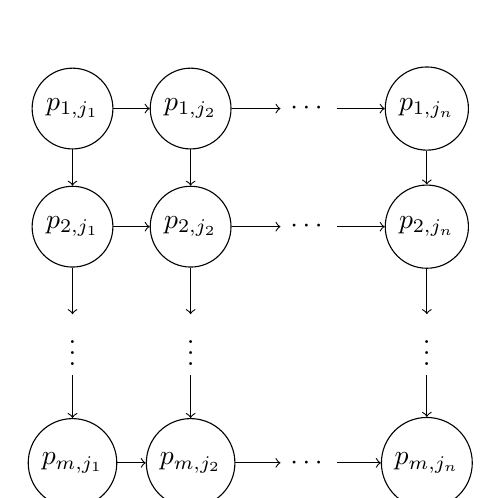
\begin{tikzpicture}              
        \node [circle, draw=black] (11) at (0, 8) {$p_{1,j_1}$};  
        \node [circle, draw=black] (12) at (1.5, 8) {$p_{1,j_2}$}; 
        \node (13) at (3, 8) {$\cdots$}; 
        \node [circle, draw=black] (14) at (4.5, 8) {$p_{1,j_n}$}; 
        
        \node [circle, draw=black] (21) at (0, 6.5) {$p_{2,j_1}$};
        \node [circle, draw=black] (22) at (1.5, 6.5) {$p_{2,j_2}$};
        \node (23) at (3, 6.5) {$\cdots$};
        \node [circle, draw=black] (24) at (4.5, 6.5) {$p_{2,j_n}$}; 
        
        \node (31) at (0, 5) {$\vdots$};
        \node (32) at (1.5, 5) {$\vdots$};
        \node (34) at (4.5, 5) {$\vdots$};

        \node [circle, draw=black] (41) at (0, 3.5) {$p_{m,j_1}$};
        \node [circle, draw=black] (42) at (1.5, 3.5) {$p_{m,j_2}$};
        \node (43) at (3, 3.5) {$\cdots$};
        \node [circle, draw=black] (44) at (4.5, 3.5) {$p_{m,j_n}$};
        
        \draw [->] (11) -- (12); \draw [->] (12) -- (13); \draw [->] (13) -- (14);
        \draw [->] (21) -- (22); \draw [->] (22) -- (23); \draw [->] (23) -- (24);
        \draw [->] (41) -- (42); \draw [->] (42) -- (43); \draw [->] (43) -- (44);
        \draw [->] (11) -- (21); \draw [->] (21) -- (31); \draw [->] (31) -- (41);
        \draw [->] (12) -- (22); \draw [->] (22) -- (32); \draw [->] (32) -- (42);
        \draw [->] (14) -- (24); \draw [->] (24) -- (34); \draw [->] (34) -- (44);
    \end{tikzpicture} 
\end{center}

\begin{exmp}{exmp:7.1}
    Consider $n = 5$ jobs on $m = 4$ machines with the processing times below. 
    \begin{align*}
        \begin{array}{c|ccccc}
            \text{Jobs} & j_1 & j_2 & j_3 & j_4 & j_5 \\ \hline 
            p_{1,j_k} & 5 & 5 & 3 & 6 & 3 \\ 
            p_{2,j_k} & 4 & 4 & 2 & 4 & 4 \\ 
            p_{3,j_k} & 4 & 4 & 3 & 4 & 1 \\ 
            p_{4,j_k} & 3 & 6 & 3 & 2 & 5             
        \end{array}
    \end{align*}
    Under the sequence $j_1, j_2, j_3, j_4, j_5$, the corresponding 
    graph and Gantt chart are given below. 
    In the top right corner of each node in the directed graph, we put the 
    completion time of that node. It follows that the makespan is 
    $C_{\max} = 34$, and it is determined by the two critical paths given in red.
    \begin{center}
        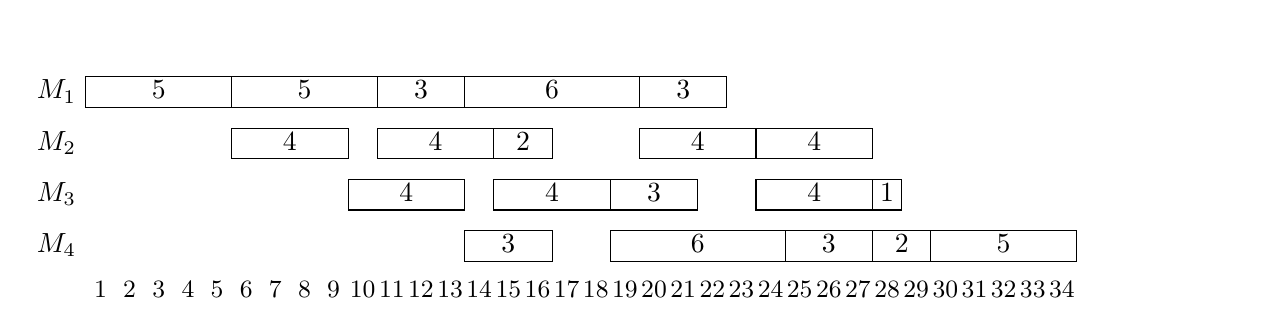
\begin{tikzpicture}[/pgfgantt/y unit chart=0.65cm] 
            \begin{ganttchart}[
                title/.style={draw=none},
                canvas/.append style={draw=none}, 
                bar top shift=0.1, bar height=0.6,
                y unit title=0.65cm,
                x unit=0.37cm
            ]{1}{40}
                \ganttbar{$M_1$}{1}{5} \ganttbar[inline]{5}{1}{5} \ganttbar[inline]{5}{6}{10} \ganttbar[inline]{3}{11}{13} \ganttbar[inline]{6}{14}{19} \ganttbar[inline]{3}{20}{22} \\ 
                \ganttbar{$M_2$}{6}{9} \ganttbar[inline]{4}{6}{9} \ganttbar[inline]{4}{11}{14} \ganttbar[inline]{2}{15}{16} \ganttbar[inline]{4}{20}{23} \ganttbar[inline]{4}{24}{27} \\ 
                \ganttbar{$M_3$}{10}{13} \ganttbar[inline]{4}{10}{13} \ganttbar[inline]{4}{15}{18} \ganttbar[inline]{3}{19}{21} \ganttbar[inline]{4}{24}{27} \ganttbar[inline]{1}{28}{28} \\ 
                \ganttbar{$M_4$}{14}{16} \ganttbar[inline]{3}{14}{16} \ganttbar[inline]{6}{19}{24} \ganttbar[inline]{3}{25}{27} \ganttbar[inline]{2}{28}{29} \ganttbar[inline]{5}{30}{34} \\ 
                \gantttitlelist{1,...,34}{1}
            \end{ganttchart}
        \end{tikzpicture}
        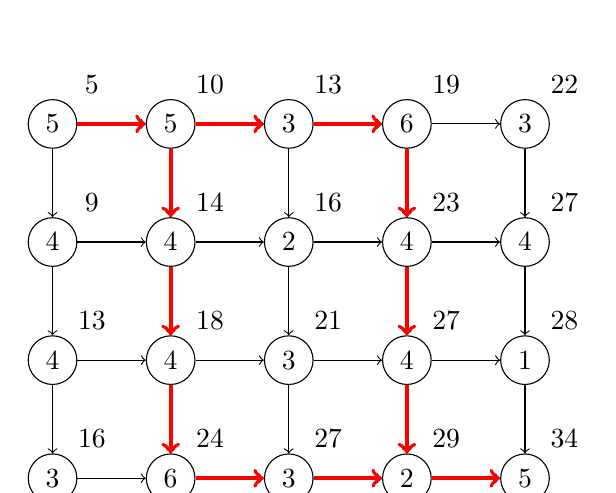
\begin{tikzpicture}              
            \node [circle, draw=black] (11) at (0, 8) {$5$};  
            \node [circle, draw=black] (12) at (1.5, 8) {$5$}; 
            \node [circle, draw=black] (13) at (3, 8) {$3$}; 
            \node [circle, draw=black] (14) at (4.5, 8) {$6$}; 
            \node [circle, draw=black] (15) at (6, 8) {$3$}; 
            
            \node [circle, draw=black] (21) at (0, 6.5) {$4$};
            \node [circle, draw=black] (22) at (1.5, 6.5) {$4$};
            \node [circle, draw=black] (23) at (3, 6.5) {$2$};
            \node [circle, draw=black] (24) at (4.5, 6.5) {$4$};
            \node [circle, draw=black] (25) at (6, 6.5) {$4$};
            
            \node [circle, draw=black] (31) at (0, 5) {$4$};
            \node [circle, draw=black] (32) at (1.5, 5) {$4$};
            \node [circle, draw=black] (33) at (3, 5) {$3$};
            \node [circle, draw=black] (34) at (4.5, 5) {$4$};
            \node [circle, draw=black] (35) at (6, 5) {$1$};
            
            \node [circle, draw=black] (41) at (0, 3.5) {$3$};
            \node [circle, draw=black] (42) at (1.5, 3.5) {$6$};
            \node [circle, draw=black] (43) at (3, 3.5) {$3$};
            \node [circle, draw=black] (44) at (4.5, 3.5) {$2$};
            \node [circle, draw=black] (45) at (6, 3.5) {$5$};
            
            \node (11') at (0.5, 8.5) {$5$};
            \node (12') at (2, 8.5) {$10$};
            \node (13') at (3.5, 8.5) {$13$};
            \node (14') at (5, 8.5) {$19$};
            \node (15') at (6.5, 8.5) {$22$};
            
            \node (21') at (0.5, 7) {$9$};
            \node (22') at (2, 7) {$14$};
            \node (23') at (3.5, 7) {$16$};
            \node (24') at (5, 7) {$23$};
            \node (25') at (6.5, 7) {$27$};
            
            \node (31') at (0.5, 5.5) {$13$};
            \node (32') at (2, 5.5) {$18$};
            \node (33') at (3.5, 5.5) {$21$};
            \node (34') at (5, 5.5) {$27$};
            \node (35') at (6.5, 5.5) {$28$};
            
            \node (41') at (0.5, 4) {$16$};
            \node (42') at (2, 4) {$24$};
            \node (43') at (3.5, 4) {$27$};
            \node (44') at (5, 4) {$29$};
            \node (45') at (6.5, 4) {$34$};
            
            \foreach \x in {1,...,4}
            { 
                \foreach \y in {1,...,4}
                {
                    \pgfmathtruncatemacro{\cur}{10*\x + \y}
                    \pgfmathtruncatemacro{\next}{\cur + 1}
                    \draw [->] (\cur) -- (\next); 
                }
            }
            
            \foreach \x in {1,...,3}
            { 
                \foreach \y in {1,...,5}
                {
                    \pgfmathtruncatemacro{\curvert}{10*\x + \y}
                    \pgfmathtruncatemacro{\nextvert}{\curvert + 10}
                    \draw [->] (\curvert) -- (\nextvert); 
                }
            }
            
            \draw[->, draw=red, line width=0.5mm] (11) -- (12);
            \draw[->, draw=red, line width=0.5mm] (12) -- (13);
            \draw[->, draw=red, line width=0.5mm] (13) -- (14);
            \draw[->, draw=red, line width=0.5mm] (12) -- (22);
            \draw[->, draw=red, line width=0.5mm] (22) -- (32);
            \draw[->, draw=red, line width=0.5mm] (32) -- (42);
            \draw[->, draw=red, line width=0.5mm] (14) -- (24);
            \draw[->, draw=red, line width=0.5mm] (24) -- (34);
            \draw[->, draw=red, line width=0.5mm] (34) -- (44);
            \draw[->, draw=red, line width=0.5mm] (42) -- (43);
            \draw[->, draw=red, line width=0.5mm] (43) -- (44);
            \draw[->, draw=red, line width=0.5mm] (44) -- (45);
        \end{tikzpicture} 
    \end{center}
\end{exmp}

\subsection{Johnson's Rule} \label{subsec:7.2}
We now consider the $(F_2~||~C_{\max})$ problem. Note that there 
is no permutation schedule restriction here, as we noted that 
$(F_2~||~C_{\max})$ has an optimal schedule that is a permutation schedule. 
There are two machines and $n$ jobs, with processing time $a_j = p_{1j}$ on 
machine $1$ and processing time $b_j = p_{2j}$ on machine $2$. This was one of 
the first problems to be analyzed in the early days of operations research 
and led to a classical paper in scheduling theory by S. M. Johnson. 
The rule that minimizes the makespan is commonly referred to as 
Johnson's rule. 

\begin{algo}[Johnson's rule]{algo:7.2}
    \begin{enumerate}[(1)]
        \item Set $i = 1$, $\ell = n$, and $\hat J = [n]$. 
        \item If $\hat J = \varnothing$, then stop. Otherwise, set 
        $\mu = \min\{a_j, b_j : j \in \hat J\}$. 
        \item \begin{enumerate}[(a)]
            \item If $\mu = a_j$, then place job $j$ in position $i$
            of the sequence. Increase $i$ by $1$ and delete $j$ from 
            $\hat J$. Go back to Step 2. 
            \item If $\mu = b_j$, then place job $j$ in position $\ell$
            of the sequence. Decrease $\ell$ by $1$ and delete $j$ from 
            $\hat J$. Go back to Step 2. 
        \end{enumerate} 
    \end{enumerate}
\end{algo}

\begin{exmp}{exmp:7.3}
    Consider the following $n = 5$ jobs on two machines. 
    \begin{align*}
        \begin{array}{c|ccccc}
            j & 1 & 2 & 3 & 4 & 5 \\ \hline 
            a_j & 5 & 2 & 3 & 6 & 3 \\ 
            b_j & 1 & 4 & 3 & 4 & 4
        \end{array}
    \end{align*}
    Then at iteration 1, we have $\mu = b_1 = 1$, so we put job $1$ 
    in position $5$. At iteration 2, we have $\mu = a_2 = 2$, so we put 
    job $2$ in position $1$. At iteration 3, we arbitrarily pick 
    $\mu = a_3 = 3$, so job $3$ goes in position $2$. At iteration 4, 
    we get $\mu = a_5 = 3$, so job $5$ goes in position $3$. Finally, job 
    $4$ goes in position $4$, so we obtain the final sequence 
    $2, 3, 5, 4, 1$. 
\end{exmp}

Note that Johnson's rule is equivalent to the following algorithm. 
Partition the jobs into two sets: $S_1$ contains all jobs $j$ with 
$a_j \leq b_j$, and $S_2$ contains all jobs $j$ with $a_j > b_j$. 
Place the jobs in $S_1$ first in SPT order, and the jobs in $S_2$ last 
in LPT order. In this sense, this is also called the SPT(1)-LPT(2) rule. 

Let us now show that Johnson's rule is indeed optimal for 
$(F_2~||~C_{\max})$. We first prove a key lemma. 

\begin{lemma}{lemma:7.4}
    \begin{enumerate}[(1)]
        \item If $\mu = a_j = \min\{a_\ell, b_\ell : \ell \in [n]\}$ in the 
        first iteration of Johnson's rule, then there is an optimal schedule 
        that places job $j$ first. 
        \item If $\mu = b_j = \min\{a_\ell, b_\ell : \ell \in [n]\}$ in the 
        first iteration of Johnson's rule, then there is an optimal schedule 
        that places job $j$ last. 
    \end{enumerate}
\end{lemma}
\begin{pf}
    We will only prove (1), as the proof of (2) is analogous. 
    Suppose that we have an optimal schedule $S^*$ that does not start with 
    job $j$. Then there must be a job $\ell$ immediately preceding $j$ in 
    $S$. Let $t_\ell^1$ denote the starting time of $\ell$ on machine $1$, 
    and let $t_\ell^2$ denote the starting time of $\ell$ on machine $2$. 
    We interchange jobs $j$ and $\ell$ to get a new schedule $S'$. 

    We claim that $C'_\ell \leq C_j$, where $C'_\ell$ is the completion time 
    of job $\ell$ in $S'$ and $C_j$ is the completion time of job $j$ in $S$. 
    Observe that in the directed graph representation under $S$, 
    there are three possible paths we could take, illustrated below. 
    \begin{center}
        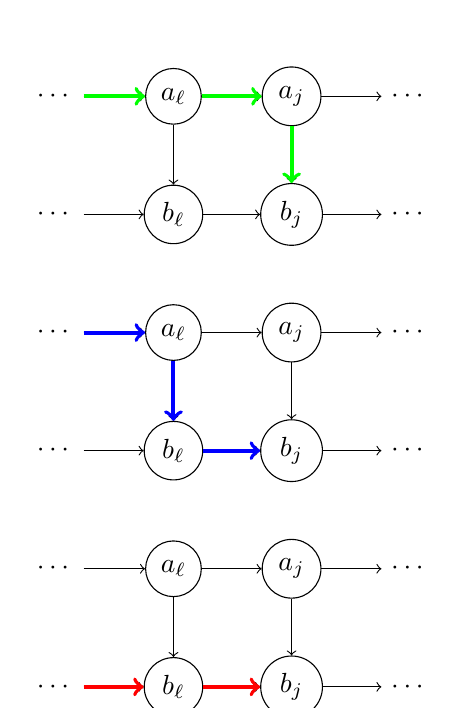
\begin{tikzpicture}              
            \node (111) at (0, 8) {$\cdots$};  
            \node [circle, draw=black] (112) at (1.5, 8) {$a_\ell$}; 
            \node [circle, draw=black] (113) at (3, 8) {$a_j$}; 
            \node (114) at (4.5, 8) {$\cdots$}; 
            
            \node (121) at (0, 6.5) {$\cdots$};  
            \node [circle, draw=black] (122) at (1.5, 6.5) {$b_\ell$}; 
            \node [circle, draw=black] (123) at (3, 6.5) {$b_j$}; 
            \node (124) at (4.5, 6.5) {$\cdots$}; 
            
            \node (211) at (0, 5) {$\cdots$};  
            \node [circle, draw=black] (212) at (1.5, 5) {$a_\ell$}; 
            \node [circle, draw=black] (213) at (3, 5) {$a_j$}; 
            \node (214) at (4.5, 5) {$\cdots$}; 
            
            \node (221) at (0, 3.5) {$\cdots$};  
            \node [circle, draw=black] (222) at (1.5, 3.5) {$b_\ell$}; 
            \node [circle, draw=black] (223) at (3, 3.5) {$b_j$}; 
            \node (224) at (4.5, 3.5) {$\cdots$}; 
            
            \node (311) at (0, 2) {$\cdots$};  
            \node [circle, draw=black] (312) at (1.5, 2) {$a_\ell$}; 
            \node [circle, draw=black] (313) at (3, 2) {$a_j$}; 
            \node (314) at (4.5, 2) {$\cdots$}; 
            
            \node (321) at (0, 0.5) {$\cdots$};  
            \node [circle, draw=black] (322) at (1.5, 0.5) {$b_\ell$}; 
            \node [circle, draw=black] (323) at (3, 0.5) {$b_j$}; 
            \node (324) at (4.5, 0.5) {$\cdots$}; 

            \draw [->] (111) -- (112); \draw [->] (112) -- (113); \draw [->] (113) -- (114); 
            \draw [->] (121) -- (122); \draw [->] (122) -- (123); \draw [->] (123) -- (124);
            \draw [->] (112) -- (122); \draw [->] (113) -- (123); 

            \draw [->] (211) -- (212); \draw [->] (212) -- (213); \draw [->] (213) -- (214); 
            \draw [->] (221) -- (222); \draw [->] (222) -- (223); \draw [->] (223) -- (224);
            \draw [->] (212) -- (222); \draw [->] (213) -- (223); 

            \draw [->] (311) -- (312); \draw [->] (312) -- (313); \draw [->] (313) -- (314); 
            \draw [->] (321) -- (322); \draw [->] (322) -- (323); \draw [->] (323) -- (324);
            \draw [->] (312) -- (322); \draw [->] (313) -- (323); 
            
            \draw[->, draw=green, line width=0.5mm] (111) -- (112);
            \draw[->, draw=green, line width=0.5mm] (112) -- (113);
            \draw[->, draw=green, line width=0.5mm] (113) -- (123);

            \draw[->, draw=blue, line width=0.5mm] (211) -- (212);
            \draw[->, draw=blue, line width=0.5mm] (212) -- (222);
            \draw[->, draw=blue, line width=0.5mm] (222) -- (223);

            \draw[->, draw=red, line width=0.5mm] (321) -- (322);
            \draw[->, draw=red, line width=0.5mm] (322) -- (323);
        \end{tikzpicture} 
    \end{center}
    Note that the green path is dominated by the blue path because 
    $a_j \leq b_\ell$ by assumption. This shows that 
    \[ C_j = \max\{t_\ell^2 + b_\ell + b_j, t_\ell^1 + a_\ell + b_\ell + b_j\}. \] 
    Constructing a similar diagram for $S'$ gives us 
    \[ C'_\ell = \max\{t_\ell^1 + a_j + a_\ell + b_\ell, 
    t_\ell^1 + a_j + b_j + b_\ell, 
    t_\ell^2 + b_j + b_\ell\}. \] 
    Noting that $a_j = \min\{a_j, b_j : j \in [n]\}$, it is easy to 
    check that $C_j \geq C'_\ell$ by comparing the terms above. 
    This means that $S'$ is also an optimal schedule which has job $j$ 
    before job $\ell$. We can continue to interchange jobs and 
    repeat our argument until job $j$ is first. 
\end{pf}

\begin{theo}{theo:7.5}
    Johnson's rule gives an optimal schedule for $(F_2~||~C_{\max})$. 
\end{theo}
\begin{pf}
    We give a sketch of the proof. We proceed by induction on the number 
    of iterations. The earlier iterations would have constructed a 
    partial schedule. Apply Lemma~\ref{lemma:7.4} to the set of jobs 
    that remain to be scheduled after $i-1$ iterations. Note that 
    Lemma~\ref{lemma:7.4} only sees the two jobs $j$ minimizing the 
    value of $\mu$ and the job $\ell$ immediately preceding job $j$; 
    it ``ignores'' all other jobs. 
\end{pf}

As one might imagine, a schedule obtained from Johnson's rule is 
by no means the only schedule that is optimal for $(F_2~||~C_{\max})$. 
The class of optimal schedules appears to be hard to characterize and 
data dependent. 

\subsection{Mixed Integer Program Formulation for Permutation Schedules} \label{subsec:7.3}
Unfortunately, the schedule structure from Johnson's rule cannot be 
generalized to characterize optimal schedules for flow shops with 
more than two machines. Indeed, it turns out that even the three machine case 
is strongly $\NP$-hard. 

\begin{theo}{theo:7.6}
    The problem $(F_3~||~C_{\max})$ is strongly $\NP$-hard. 
\end{theo}
\begin{pf}
    We prove this via a reduction from \textsc{$3$-Partition}. Given 
    $a_1, \dots, a_{3t}, b \in \Z^+$ under the usual assumptions, 
    let the number of jobs be $n = 4t+1$, and let the processing times be 
    \begin{align*}
        p_{10} &= 0, & p_{20} &= b, & p_{30} &= 2b, \\ 
        p_{1j} &= 2b, & p_{2j} &= b, & p_{3j} &= 2b, & j &= 1, \dots, t-1, \\ 
        p_{1t} &= 2b, & p_{2t} &= b, & p_{3t} &= 3b, \\ 
        p_{1,t+j} &= 0, & p_{2,t+j} &= a_j, & p_{3,t+j} &= 0, & j &= 1, \dots, 3t. 
    \end{align*}
    Let $z = (2t+1)b$. A makespan of value $z$ can be obtained if the first 
    $t+1$ jobs are scheduled according to the sequence $0, 1, \dots, t$. 
    These $t+1$ jobs then form a framework, leaving $t$ gaps on machine $2$. 
    Then jobs $t+1, \dots, 4t$ have to be partitioned into $t$ sets of three 
    jobs each, and these $t$ sets have to be scheduled between the first 
    $t+1$ jobs. Thus, a makespan of $z$ can be obtained if and only if 
    the \textsc{$3$-Partition} instance has a solution. 
\end{pf}

The problem $(F_m~|~\text{prmu}~|~C_{\max})$ can be formulated 
as a mixed integer program (MIP). Note that the fact that the problem 
can be formulated in this way does not imply that the problem is 
$\NP$-hard. It could be that the MIP has a special structure that 
allows for a polynomial time algorithm, such as the one we saw 
for $(R_m~||~\sum C_j)$ in Section~\ref{subsec:6.4}. However, 
Theorem~\ref{theo:7.6} shows that this is not the case. 

We first define some variables that we need.
\begin{itemize}
    \item Let $x_{jk}$ be a binary variable equal to $1$ if job $j$ is the 
    $k$-th job in the sequence, and $0$ otherwise. 
    \item The auxiliary variable $I_{ik}$ denotes the idle time on machine $i$
    between the processing of the jobs in the $k$-th and $(k+1)$-th positions. 
    \item The auxiliary variable $W_{ik}$ denotes the waiting time of the 
    job in the $k$-th position between machines $i$ and $i+1$. 
\end{itemize} 
Naturally, there is a strong relationship between the variables $W_{ik}$ and 
the variables $I_{ik}$. For example, if $I_{ik} > 0$, then 
$W_{i-1,k+1} = 0$. Formally, this relationship can be established by 
considering the difference between the time the job in the $(k+1)$-th 
position starts on machine $i+1$ and the time the job in the $k$-th position 
completes its processing on machine $i$. If $\Delta_{ik}$ denotes this 
difference and $p_{i(k)}$ is the processing time of the job in the 
$k$-th position on machine $i$, then 
\[ \Delta_{ik} = I_{ik} + p_{i(k+1)} + W_{i,k+1} = W_{ik} + p_{i+1(k)} 
+ I_{i+1,k}. \] 
Note that minimizing the makespan is equivalent to minimizing the 
total idle time on the last machine, namely machine $m$. This idle 
time is equal to 
\[ \sum_{i=1}^{m-1} p_{i(1)} + \sum_{j=1}^{n-1} I_{mj}, \] 
which is the idle time that must occur before the job in the first position 
reaches the last machine and the sum of the idle times between the jobs 
on the last machine. Moreover, we have the identity
\[ p_{i(k)} = \sum_{j=1}^n x_{jk} p_{ij}. \] 
Putting everything together, we can now formulate the MIP as follows: 
\begin{align*}
    \min\quad & \sum_{i=1}^{m-1} \sum_{j=1}^n x_{j1} p_{ij} + \sum_{j=1}^{n-1} I_{mj} \\ 
    \text{s.t.}\quad & \sum_{j=1}^n x_{jk} = 1, && k \in [n] \\ 
    & \sum_{k=1}^n x_{jk} = 1, && j \in [n] \\ 
    & I_{ik} + \sum_{j=1}^n x_{j,k+1} p_{ij} + W_{i,k+1} - W_{ik} 
    - \sum_{j=1}^n x_{jk} p_{i+1,j} - I_{i+1,k} = 0, && k \in [n-1],\; i \in [m-1] \\
    & W_{i1} = 0, && i \in [m-1] \\
    & I_{1k} = 0, && k \in [n-1].
\end{align*}
The first set of constraints specifies that exactly one job has to be assigned to
position $k$ for any $k$. The second set of constraints specifies that job $j$ has to be
assigned to exactly one position. The third set of constraints relate the decision
variables $x_{jk}$ to the physical constraints. These physical constraints enforce the
necessary relationships between the idle time variables and the waiting time
variables. Thus, the problem of minimizing the makespan in an $m$ machine
permutation flow shop is formulated as an MIP. The only integer variables
are the binary decision variables $x_{jk}$. The idle time and waiting time
variables are non-negative continuous variables.\newpage
\section{Open Shops} \label{sec:8}
Recall that in a flow shop, each job must follow the same route. 
In the next section, we will also discuss job shops, where each job has its 
own predetermined fixed route. However, in practice, it is often the case that 
the route of the job is immaterial and up to the schedule to decide. The 
routes of the job are \emph{open} in this sense, and this model is called 
an open shop. But we still have the usual restrictions that each machine 
can only handle one job at a time, and two operations of the same job 
cannot be run at the same time. 

\subsection{Makespan without Preemptions} \label{subsec:8.1}
We first consider the $(O_2~||~C_{\max})$ problem where there are 
two machines. A job $j$ can be processed first on machine $1$ or 
vice versa; the decision maker can determine the routes. It is clear that 
\[ C_{\max} \geq \max\left( \sum_{j=1}^n p_{1j}, \sum_{j=1}^n p_{2j} \right), \] 
since the makespan cannot be less than the workload on either machine. 

One might expect that this is an equality, and this is true 
in most situations. However, to get equality, we must also consider 
$\max_{j\in[n]} p_{1j} + p_{2j}$ because of the restriction 
that two operations of the same job cannot be run at the same time. 
Thus, the optimal makespan is 
\[ C_{\max} = \max\left( \max_{j\in[n]} (p_{1j} + p_{2j}), 
\sum_{j=1}^n p_{1j}, \sum_{j=1}^n p_{2j} \right). \] 
For now, we only consider non-delay schedules. That is, if there is a job 
waiting for processing when a machine is free, then that machine is 
not allowed to remain idle. It follows that an idle period can occur 
on a machine if and only if one job remains to be processed on that machine 
and when that machine is available, this last job is still being processed 
on the other machine. Such an idle period \emph{can} cause an unnecessary 
increase in the makespan. If this last job turns out to be the very last 
job to complete all its processing, then the idle period does cause 
an increase in the makespan. But if this last job, after having 
completed its processing on the machine that was idle, is \emph{not} 
the very last job to leave the system, then the makespan is still 
equal to the maximum of the two workloads. 

We now give an algorithm that solves $(O_2~||~C_{\max})$ instances in 
polynomial time. We may assume without loss of generality that the 
longest processing time among the $2n$ processing times belongs to 
operation $(1, k)$, because we can swap the two machines if needed. 
That is, we have $p_{ij} \leq p_{1k}$ for all $i = 1, 2$ and 
$j = 1, \dots, n$. 

\begin{algo}{algo:8.1}
    If operation $(1, k)$ is the longest operation, then job $k$ must be 
    started at time $0$ on machine $2$.
    After job $k$ has completed its processing on machine $2$, 
    its operation $(1, k)$ has the lowest possible priority with 
    regard to processing on machine $1$. Then the processing of 
    operation $(1, k)$ will be postponed as much as possible; 
    it can only be processed on machine $1$ if no other job is 
    available for processing on machine $1$. (This can only 
    happen either if it is the last operation to be done on 
    machine $1$, or if it is the second last operation and the 
    last operation is not available because it is still being 
    processed on machine $2$.) The $2(n-1)$ operations 
    of the remaining $n-1$ jobs can be processed on the two machines 
    in any order. However, unforced idleness is not allowed. 
\end{algo} 

Algorithm~\ref{algo:8.1} is a more general form of the 
{\bf Longest Alternate Processing Time first (LAPT)} rule, which says 
that whenever a machine is freed, start processing the jobs that have 
not yet received processing on either machine the one with the longest 
processing time on the \emph{other} machine. 

\begin{theo}{theo:8.2}
    Algorithm~\ref{algo:8.1} results in an optimal schedule for 
    $(O_2~||~C_{\max})$ with makespan 
    \[ C_{\max} = \max\left( \max_{j\in[n]} (p_{1j} + p_{2j}), 
    \sum_{j=1}^n p_{1j}, \sum_{j=1}^n p_{2j} \right). \] 
\end{theo}
\begin{pf}
    If the resulting schedule has no idle period on either machine, then 
    it is of course optimal. However, an idle period may occur either on 
    machine $1$ or on machine $2$. We consider two cases. 

    {\sc Case 1.} Suppose an idle period occurs on machine $2$. 
    If this is the case, then only one more operation needs processing on 
    machine $2$ but this operation still has to complete its processing 
    on machine $1$. Assume that this operation belongs to job $\ell$. 
    When job $\ell$ starts on machine $2$, job $k$ starts on machine $1$
    and $p_{1k} > p_{2\ell}$. Hence, the makespan is determined by the 
    completion of job $k$ on machine $1$ and no idle period has occurred 
    on machine $1$. This means the schedule is optimal. 

    {\sc Case 2.} Suppose an idle period occurs on machine $1$. An idle period 
    on machine $1$ can occur only when machine $1$ is freed after completing 
    all its operations with the exception of operation $(1, k)$, and operation 
    $(2, k)$ of job $k$ is still being processed on machine $2$ at that point. 
    In this case, the makespan is equal to $p_{2k} + p_{1k}$ and the schedule 
    is optimal.
\end{pf}

The LAPT rule we described above can be considered to be a special case 
of a more general rule that can be applied to open shops with more than 
two machines. This rule is called the {\bf Longest Total Remaining 
Processing on Other Machines first (LTRPOM)} rule. According to this rule, 
the processing required on the machine currently available does not 
affect the priority level of a job. However, this rule does not always 
result in an optimal schedule because the $(O_m~||~C_{\max})$ problem is 
$\NP$-hard when $m \geq 3$. 

\begin{theo}{theo:8.3}
    The $(O_3~||~C_{\max})$ problem is weakly $\NP$-hard. 
\end{theo}
\begin{pf}
    We prove this using a reduction from {\sc Partition} to 
    $(O_3~||~C_{\max})$. Given $a_1, \dots, a_t, b \in \Z^+$ such that 
    $\sum_{j=1}^t a_j = 2b$, we construct $n = 3t + 1$ jobs. There are three 
    jobs corresponding to each value $a_j$, given by 
    \begin{align*}
        p_{1j} &= a_j, & p_{2j} &= 0, & p_{3j} &= 0, & j &= 1, \dots, t, \\
        p_{1j} &= 0, & p_{2j} &= a_j, & p_{3j} &= 0, & j &= t+1, \dots, 2t, \\
        p_{1j} &= 0, & p_{2j} &= 0, & p_{3j} &= a_j, & j &= 2t+1, \dots, 3t.
    \end{align*}
    There is one more marker job with processing times 
    \[ p_{1,3t+1} = p_{2,3t+1} = p_{3,3t+1} = b. \] 
    Let $z^* = 3b$. We claim that there is a schedule with makespan 
    $z^*$ if and the {\sc Partition} instance has a solution. 
    Suppose there is a schedule with makespan $z^* = 3b$. Assume 
    without loss of generality that the marker job $3t+1$ is scheduled 
    on time interval $[b, 2b]$ on machine $1$, because we could swap 
    machines otherwise. Then the jobs processed at time interval 
    $[0, b]$ on machine $1$ correspond to a subset $S_1 \subseteq 
    \{1, \dots, t\}$ such that $\sum_{j\in S_1} a_j = b$, 
    as do the jobs processed at time interval $[2b, 3b]$ on machine $2$. 
    Thus, the {\sc Partition} instance has a solution. 
 
    Suppose that the {\sc Partition} instance has a solution, namely a 
    partition $(S_1, S_2)$ of $\{1, \dots, t\}$ such that 
    $\sum_{j\in S_1} a_j = \sum_{j\in S_2} a_j = b$. Process 
    job $3t+1$ on machine $2$ at time interval $[0, b]$, on machine 
    $1$ at time interval $[b, 2b]$, and on machine $3$ at time interval 
    $[2b, 3b]$. Then we could place all jobs in $S_1$ on machine $1$ 
    at time interval $[0, b]$ and all jobs in $S_2$ on machine $1$ 
    at time interval $[2b, 3b]$. This will extend naturally to a schedule 
    with makespan $z^* = 3b$. 
\end{pf}

The schedule from the proof of Theorem~\ref{theo:8.3} is described 
in the following Gantt chart. 
\begin{center}
    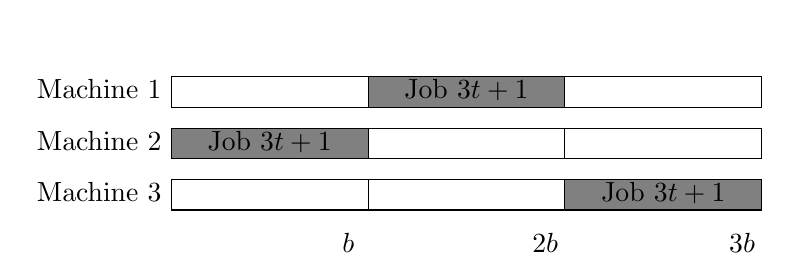
\begin{tikzpicture}[/pgfgantt/y unit chart=0.65cm] 
        \begin{ganttchart}[
            title/.style={draw=none},
            canvas/.append style={draw=none}, 
            bar top shift=0.1, bar height=0.6,
            y unit title=0.65cm,
        ]{1}{15}
            \ganttbar{Machine 1}{1}{5} \ganttbar[inline]{}{1}{5} \ganttbar[inline, bar/.append style={fill=gray}]{Job $3t+1$}{6}{10} \ganttbar[inline]{}{11}{15} \\ 
            \ganttbar{Machine 2}{1}{5} \ganttbar[inline, bar/.append style={fill=gray}]{Job $3t+1$}{1}{5} \ganttbar[inline]{}{6}{10} \ganttbar[inline]{}{11}{15} \\ 
            \ganttbar{Machine 3}{1}{5} \ganttbar[inline]{}{1}{5} \ganttbar[inline]{}{6}{10} \ganttbar[inline, bar/.append style={fill=gray}]{Job $3t+1$}{11}{15} \\ 
            \ganttbar[inline, bar/.style={draw=none}]{$b$}{5}{5} \ganttbar[inline, bar/.style={draw=none}]{$2b$}{10}{10} \ganttbar[inline, bar/.style={draw=none}]{$3b$}{15}{15}
        \end{ganttchart}
    \end{tikzpicture}
\end{center}   
\vspace{-0.4cm}
Algorithm~\ref{algo:8.1} is one of the few polynomial time algorithms 
for non-preemptive open shop problems. Most of the more general open shop 
models are $\NP$-hard, such as $(O_2~|~r_j~|~C_{\max})$. However, it turns 
out that the problem $(O_m~|~r_j, p_{ij} = 1~|~C_{\max})$ can be solved 
in polynomial time. We discuss this further in Section~\ref{subsec:8.3}. 

\subsection{Makespan with Preemptions} \label{subsec:8.2} 
Preemptive open shop problems tend to be somewhat easier. In contrast 
to the $(O_m~||~C_{\max})$ problem, we will see that the 
$(O_m~|~\text{prmp}~|~C_{\max})$ problem is solvable in polynomial time. 

Note that the value of the makespan under Algorithm~\ref{algo:8.1} 
(or LAPT) is a lower bound for the makespan with two machines, 
even when preemptions are allowed. It follows that these non-preemptive 
rules are also optimal for $(O_2~|~\text{prmp}~|~C_{\max})$. 

An easy lower bound for the makespan with $m \geq 3$ machines when 
preemptions are allowed is 
\[ C_{\max} \geq \max \left( \max_{j\in[n]} \sum_{i=1}^m p_{ij},\; 
\max_{i\in[m]} \sum_{j=1}^n p_{ij} \right). \] 
That is, the makespan must be at least as large as the maximum workload 
on each of the $m$ machines, and at least as large as the total amount 
of processing to be done on each of the $n$ jobs. It turns out that 
it is not difficult to obtain a schedule whose makespan is equal to this 
lower bound. To see how this is done, we define 
\[ \text{ML}_i = \sum_{j=1}^n p_{ij} \] 
for each $i = 1, \dots, m$ to be the load of machine $i$, and 
\[ \text{JL}_j = \sum_{i=1}^m p_{ij} \] 
for each $j = 1, \dots, n$ to be the load of job $j$. 
We can view these as the sums of the rows and columns of the 
the $m \times n$ matrix $\mathbf P$ corresponding to the processing times
$p_{ij}$. Let $\text{LB}$ be the lower bound from above. 

We call machine $i$ {\bf tight} if we have $\text{ML}_i = \text{LB}$. 
Similarly, we call job $j$ {\bf tight} if $\text{JL}_j = \text{LB}$. 
If machine $i$ or job $j$ are not tight, then they have {\bf slack}. 
A set $D$ of operations is called a {\bf decrementing set} if it contains 
one entry for each tight job, one entry for each tight machine, 
and at most one entry for each slack row and slack column. 
Similar to the matrix $\mathbf P$ of processing times, this set $D$ can be 
viewed as an $m \times n$ matrix consisting of entries from $\{0, 1\}$. 

\begin{theo}{theo:8.4}
    A decrementing set always exists and can be computed in polynomial time.
\end{theo}

We take this result for granted, but note that the proof is based on 
maximal cardinality matchings. We can use a decrementing set to 
construct a partial schedule of length $\Delta$ for some appropriately 
chosen $\Delta$. We are now ready to state the algorithm for 
$(O_m~|~\text{prmp}~|~C_{\max})$, which, finds a schedule 
with makespan $C_{\max} = \text{LB}$.

\begin{algo}{algo:8.5}
    Repeat the following steps until all operations have been successfully scheduled.
    \begin{enumerate}[(1)]
        \item Find a decrementing set $D$. 
        \item Find the maximum value of $\Delta$ such that 
        \begin{enumerate}[(i)]
            \item $\Delta \leq \min_{(i,j) \in D} p_{ij}$;
            \item $\Delta \leq \text{LB} - \text{ML}_i$ if machine $i$ 
            has slack and no operation in $D$; 
            \item $\Delta \leq \text{LB} - \text{JL}_j$ if job $j$ 
            has slack and no operation in $D$. 
        \end{enumerate}
        \item Schedule the operations in $D$ for $\Delta$ time units 
        in parallel. 
        \item Update the values of $p_{ij}$, $\text{LB}$, $\text{ML}_i$, 
        and $\text{JL}_j$. 
    \end{enumerate}
\end{algo}

Note that after each iteration, we are decreasing LB by $\Delta$, 
and a slice of $\Delta$ time units is scheduled. This suggests that 
the algorithm terminates after $\leq \text{LB}$ iterations. But we can actually 
do a slightly better analysis than this: it terminates after $\leq nm + n + m$ 
iterations. To see why, observe that at each iteration, either 
\begin{itemize}
    \item an operation gets completely scheduled, or 
    \item a slack machine or job becomes tight (and stays tight throughout 
    the later iterations).
\end{itemize}
In particular, the algorithm is polynomial time and is correct.  

\begin{exmp}{exmp:8.6}
    Consider $3$ machines and $4$ jobs with the processing times being 
    the entries in the matrix 
    \[ \mathbf P = \begin{bmatrix}
        3 & 4 & 0 & 4 \\ 
        4 & 0 & 6 & 0 \\ 
        4 & 0 & 0 & 6
    \end{bmatrix}. \] 
    We can easily see that $\text{LB} = 11$ by computing the sums of the 
    rows and columns. In particular, observe that machine $1$ 
    and job $1$ are tight, while all other machines and jobs are slack. One 
    possible decrementing set comprises of the processing times 
    $p_{12} = 4$, $p_{21} = 4$, and $p_{34} = 6$. We can choose 
    $\Delta = 4$ in this case, and a partial schedule is constructed 
    by scheduling job $2$ on machine $1$ for $4$ time units, 
    job $1$ on machine $2$ for $4$ time units, and 
    job $4$ on machine $3$ for $4$ time units. The matrix is now 
    \[ \mathbf P = \begin{bmatrix}
        3 & 0 & 0 & 4 \\ 
        0 & 0 & 6 & 0 \\ 
        4 & 0 & 0 & 2
    \end{bmatrix}, \] 
    and $\text{LB} = 7$. This means that machine $1$ and job $1$ are again 
    tight, with all other machines and jobs being slack. A decrementing set 
    is obtained with the processing times $p_{14} = 4$, $p_{23} = 6$, 
    and $p_{41} = 4$. Then for $\Delta = 4$, we can augment the partial 
    schedule by assigning job $4$ to machine $1$ for $4$ time units, 
    job $3$ to machine $2$ for $4$ time units, and job $1$ to machine $3$ 
    for $4$ time units. The matrix is updated to 
    \[ \mathbf P = \begin{bmatrix}
        3 & 0 & 0 & 0 \\ 
        0 & 0 & 2 & 0 \\ 
        0 & 0 & 0 & 2
    \end{bmatrix}. \] 
    At this point, there is an obvious way to assign the remaining 
    processing times. We can put job $1$ on machine $1$ for $3$ time units, 
    job $3$ on machine $2$ for $2$ time units, and job $4$ on machine $3$ 
    for $2$ time units.
\end{exmp}

The schedule from Example~\ref{exmp:8.6} is depicted in the following Gantt chart.
\begin{center}
    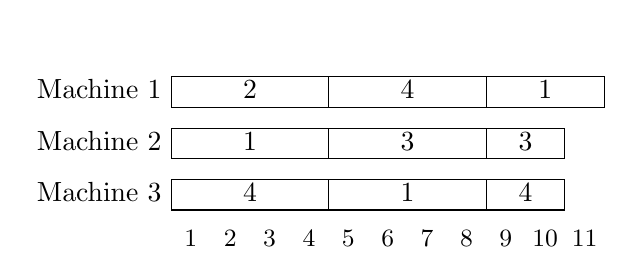
\begin{tikzpicture}[/pgfgantt/y unit chart=0.65cm] 
        \begin{ganttchart}[
            title/.style={draw=none},
            canvas/.append style={draw=none}, 
            bar top shift=0.1, bar height=0.6,
            y unit title=0.65cm,
        ]{1}{11}
            \ganttbar{Machine 1}{1}{4} \ganttbar[inline]{2}{1}{4} \ganttbar[inline]{4}{5}{8} \ganttbar[inline]{1}{9}{11} \\ 
            \ganttbar{Machine 2}{1}{4} \ganttbar[inline]{1}{1}{4} \ganttbar[inline]{3}{5}{8} \ganttbar[inline]{3}{9}{10} \\ 
            \ganttbar{Machine 3}{1}{4} \ganttbar[inline]{4}{1}{4} \ganttbar[inline]{1}{5}{8} \ganttbar[inline]{4}{9}{10} \\ 
            \gantttitlelist{1,...,11}{1}
        \end{ganttchart}
    \end{tikzpicture}
\end{center}   
\vspace{-0.4cm}

\subsection{Maximum Lateness without Preemptions} \label{subsec:8.3} 
The $(O_m~||~L_{\max})$ problem is a generalization of the 
$(O_m~||~C_{\max})$ problem, and is therefore at least as hard. 

\begin{theo}{theo:8.7}
    The problem $(O_2~||~L_{\max})$ is strongly $\NP$-hard.
\end{theo}
\begin{pf}
    We reduce \textsc{$3$-Partition} to $(O_2~||~L_{\max})$. Given 
    $a_1, \dots, a_{3t}, b \in \Z^+$ under the usual assumptions, we 
    construct $n = 4t$ jobs with processing times 
    \begin{align*}
        p_{1j} &= 0, & p_{2j} &= a_j, & d_j &= 3tb, & j &= 1, \dots, 3t, \\ 
        p_{1j} &= 0, & p_{2j} &= 2b, & d_j &= 2b, & j &= 3t+1, \\ 
        p_{1j} &= 3b, & p_{2j} &= 2b, & d_j &= (3(j-3t)-1)b, & j &= 3t+2, \dots, 4t.
    \end{align*}
    In particular, jobs $3t+1, \dots, 4t$ are marker jobs, with the 
    last job having due date $(3t-1)b$. Then there exists a schedule 
    with $L_{\max} \leq 0$ if and only if jobs $1, \dots, 3t$ can be 
    divided into $t$ groups, each containing three jobs and requiring 
    $b$ units of processing time on machine $2$. This is equivalent to 
    the \textsc{$3$-Partition} instance having a solution. 
\end{pf}

We can show that $(O_2~||~L_{\max})$ is equivalent to the 
$(O_2~|~r_j~|~C_{\max})$ problem. Indeed, consider the $(O_2~||~L_{\max})$ 
problem with deadlines $\overline{d_j}$ rather than due dates $d_j$. 
Let 
\[ \overline{d_{\max}} = \max_{j\in [n]} \overline{d_j}. \] 
Applying a time reversal to $(O_2~||~L_{\max})$, we see that finding a 
feasible schedule with $L_{\max} = 0$ is now equivalent to finding 
a schedule for $(O_2~|~r_j~|~C_{\max})$ with release dates 
\[ r_j = \overline{d_{\max}} - \overline{d_j} \] 
and a makespan that is less than $\overline{d_{\max}}$. Thus, the 
$(O_2~|~r_j~|~C_{\max})$ problem is also strongly $\NP$-hard. 

Now, we consider the special case $(O_m~|~r_j, p_{ij} = 1~|~L_{\max})$ 
that we mentioned at the end of Section~\ref{subsec:8.1}. The fact that 
all the processing times are unit makes the problem considerably easier. 
The polynomial time solution procedure consists of three phases. 
\begin{itemize}
    \item {\bf Phase 1:} Parametrizing and a binary search. 
    \item {\bf Phase 2:} Solving a network flow problem. 
    \item {\bf Phase 3:} Colouring a bipartite graph.  
\end{itemize}
At Phase 1, we let $L$ be a free parameter and assume that each job has a 
deadline $d_j + L$. The objective is to find a schedule in which each job 
is completed by its deadline, ensuring that $L_{\max} \leq L$. We set 
\[ t_{\max} = \max(d_1, \dots, d_n) + L. \] 
That is, no job should receive any processing after time $t_{\max}$. 

Phase 2 focuses on the following network flow problem. There is a source 
node $U$ that has $n$ arcs going to nodes $1, \dots, n$, where node $j$ 
corresponds to job $j$. The arc from the source node $U$ to node $j$ 
has capacity $m$, which is equal to the number of machines and the number 
of operations on each job. There is a second set of $t_{\max}$ nodes, 
with each node corresponding to one time unit. A node $t$ with 
$t = 1, \dots, t_{\max}$ represents the time slot $[t-1, t]$. A node $j$ 
has arcs going to nodes $r_j + 1, \dots, d_j + L$, and these arcs have 
unit capacity. Finally, each node in the set of $t_{\max}$ nodes 
has an arc of capacity $m$ going to the sink node $V$. This capacity limit 
ensures that no more than $m$ operations are processed in any given time 
period. The solution of this network flow problem indicates which time 
slots the $m$ operations of job $j$ need to be processed in. 
\begin{center}
    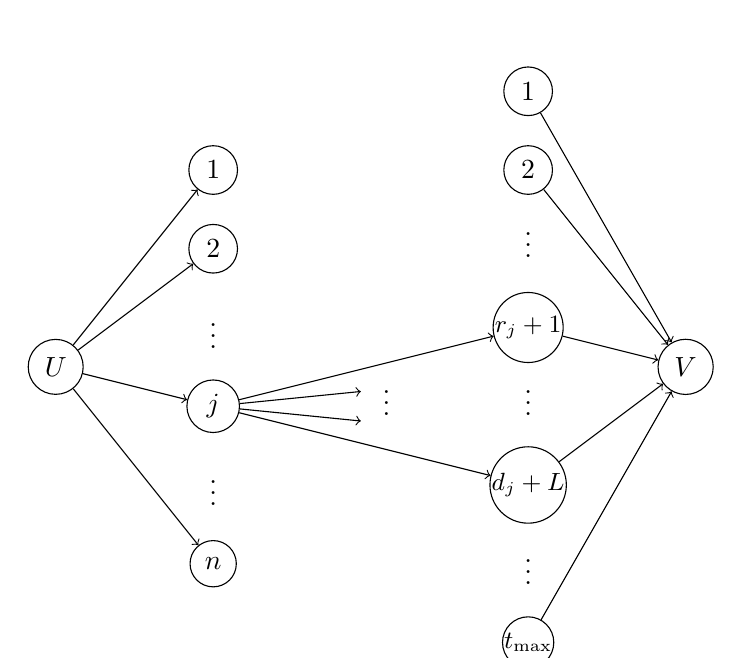
\begin{tikzpicture}              
        \node [circle, draw=black] (U) at (0, 5) {$U$};

        \node [circle, draw=black] (J1) at (2, 7.5) {$1$};
        \node [circle, draw=black] (J2) at (2, 6.5) {$2$};
        \node (Jdots1) at (2, 5.5) {$\vdots$};
        \node [circle, draw=black] (Jj) at (2, 4.5) {$j$};
        \node (Jdots2) at (2, 3.5) {$\vdots$};
        \node [circle, draw=black] (Jn) at (2, 2.5) {$n$};

        \node (blank) at (4, 4.7) {};
        \node (blank2) at (4, 4.3) {};
        \node (dots) at (4.2, 4.65) {$\vdots$};

        \node [circle, draw=black] (T1) at (6, 8.5) {$1$};
        \node [circle, draw=black] (T2) at (6, 7.5) {$2$};
        \node (Tdots1) at (6, 6.65) {$\vdots$};
        \node [circle, draw=black, inner sep=0pt, minimum size=1pt] (Trj) at (6, 5.5) {\small $r_j+1$ \normalsize};
        \node (Tdots2) at (6, 4.65) {$\vdots$};
        \node [circle, draw=black, inner sep=0pt, minimum size=1pt] (Tdj) at (6, 3.5) {\small $d_j+L$ \normalsize};
        \node (Tdots3) at (6, 2.5) {$\vdots$};
        \node [circle, draw=black, inner sep=0pt, minimum size=1pt] (Ttmax) at (6, 1.5) {\small $t_{\max}$ \normalsize};

        \node [circle, draw=black] (V) at (8, 5) {$V$};
        
        \draw [->] (U) -- (J1); \draw [->] (U) -- (J2); \draw [->] (U) -- (Jj); \draw [->] (U) -- (Jn);
        \draw [->] (T1) -- (V); \draw [->] (T2) -- (V); \draw [->] (Trj) -- (V); \draw [->] (Tdj) -- (V); \draw [->] (Ttmax) -- (V);
        \draw [->] (Jj) -- (Trj); \draw [->] (Jj) -- (Tdj);
        \draw [->] (Jj) -- (blank); \draw [->] (Jj) -- (blank2);
    \end{tikzpicture} 
\end{center}
One can also consider this network flow problem as a transportation model with 
\begin{align*}
    \min\quad & 0 \\ 
    \text{s.t.}\quad & \sum_{t=r_j+1}^{d_j+L} x_{jt} = m, && j = 1, \dots, n, \\ 
    & \sum_{j=1}^n x_{jt} \leq m, && t = 1, \dots, t_{\max}, \\ 
    & x_{jt} \leq 1, && j = 1, \dots, n,\; t = 1, \dots, t_{\max}, \\ 
    & x_{jt} \geq 0, && j = 1, \dots, n,\; t = 1, \dots, t_{\max}. 
\end{align*}
The first set of constraints ensures that for each job, all operations are 
run and are timely. The second set of constraints ensures that each time unit 
can only process at most $m$ jobs, corresponding to the number of machines. 
Note that the objective value is arbitrary here because all we need is a 
feasible solution. We recall that the unimodularity property ensures that 
an optimal solution is integer, and that such an LP can be solved in 
polynomial time. 

However, the solution to the network flow problem cannot be immediately 
translated into a feasible schedule for the open shop, because in the 
network flow formulation, no distinction is made between the different 
machines. But we can transform the assignment of operations to time slots 
prescribed by the network flow solution into a feasible schedule in 
such a way that every job $j$ is processed on a different machine 
at each time unit. 

Phase 3 of the algorithm generates a feasible schedule. From the 
solution of the network flow problem, we can construct a bipartite graph 
with two sets $N_1$ and $N_2$ of nodes. The set $N_1$ has $n$ nodes 
corresponding to the jobs, and $N_2$ has $t_{\max}$ nodes corresponding 
to the time slots. A node in $N_1$ is connected to the $m$ nodes in 
$N_2$ corresponding to the time slots in which its operations 
are supposed to be processed, prescribed by the solution from Phase 2. 
So each node in $N_1$ is connected to exactly $m$ nodes in $N_2$, 
while each node in $N_2$ is connected to at most $m$ nodes in $N_1$. 
A result in graph theory tells us that if each node in a bipartite graph 
has at most $m$ arcs, then the arcs can be coloured with $m$ different 
colours in such a way that no node has two arcs of the same colour. 
Each colour then corresponds to a machine. 

The colouring algorithm is fairly straightforward and was covered in 
MATH 239. Find a matching in the bipartite graph and colour all the 
edges in that matching with the same colour. Remove that matching 
from the graph and repeat this procedure until all edges have been coloured. 

\begin{exmp}{exmp:8.8}
    Consider the following instance of $(O_3~|~r_j, p_{ij} = 1~|~L_{\max})$ 
    with $3$ machines and $7$ jobs. 
    \begin{align*}
        \begin{array}{c|ccccccc}
            \text{Jobs} & 1 & 2 & 3 & 4 & 5 & 6 & 7 \\ \hline 
            r_j & 0 & 1 & 2 & 2 & 3 & 4 & 5 \\ 
            d_j & 5 & 5 & 5 & 6 & 6 & 8 & 8
        \end{array}
    \end{align*}
    Assume that $L = 1$. Each job has a deadline $\overline{d_j} = d_j + 1$, 
    and we have $t_{\max} = 9$. In Phase 2, we have the network flow 
    problem described below. 
    \begin{center}
        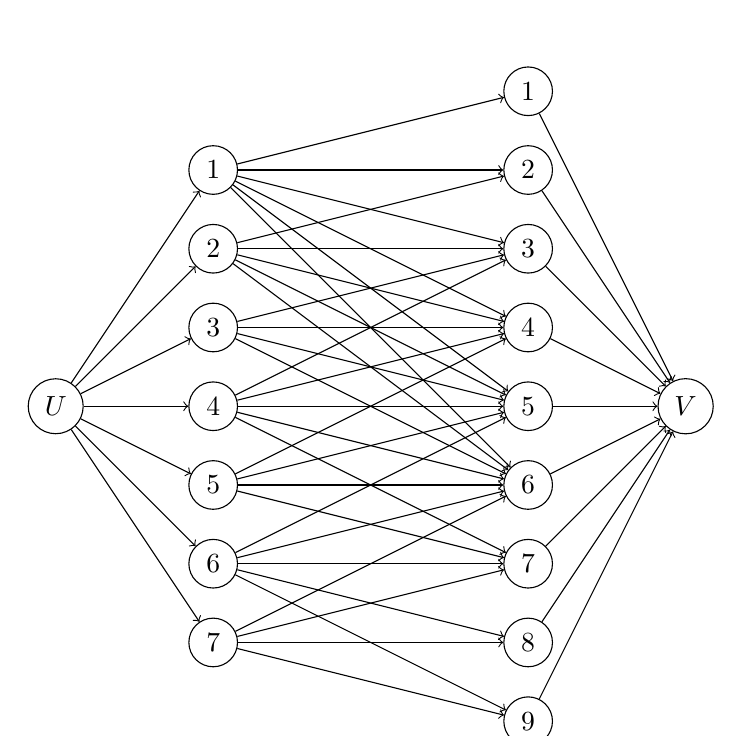
\begin{tikzpicture}              
            \node [circle, draw=black] (U) at (0, 5) {$U$};
    
            \node [circle, draw=black] (J1) at (2, 8) {$1$};
            \node [circle, draw=black] (J2) at (2, 7) {$2$};
            \node [circle, draw=black] (J3) at (2, 6) {$3$};
            \node [circle, draw=black] (J4) at (2, 5) {$4$};
            \node [circle, draw=black] (J5) at (2, 4) {$5$};
            \node [circle, draw=black] (J6) at (2, 3) {$6$};
            \node [circle, draw=black] (J7) at (2, 2) {$7$};
    
            \node [circle, draw=black] (T1) at (6, 9) {$1$};
            \node [circle, draw=black] (T2) at (6, 8) {$2$};
            \node [circle, draw=black] (T3) at (6, 7) {$3$};
            \node [circle, draw=black] (T4) at (6, 6) {$4$};
            \node [circle, draw=black] (T5) at (6, 5) {$5$};
            \node [circle, draw=black] (T6) at (6, 4) {$6$};
            \node [circle, draw=black] (T7) at (6, 3) {$7$};
            \node [circle, draw=black] (T8) at (6, 2) {$8$};
            \node [circle, draw=black] (T9) at (6, 1) {$9$};
    
            \node [circle, draw=black] (V) at (8, 5) {$V$};
            
            \draw [->] (U) -- (J1); \draw [->] (U) -- (J2); \draw [->] (U) -- (J3);
            \draw [->] (U) -- (J4); \draw [->] (U) -- (J5); \draw [->] (U) -- (J6);
            \draw [->] (U) -- (J7); 


            \draw [->] (T1) -- (V); \draw [->] (T2) -- (V); \draw [->] (T3) -- (V);
            \draw [->] (T4) -- (V); \draw [->] (T5) -- (V); \draw [->] (T6) -- (V);
            \draw [->] (T7) -- (V); \draw [->] (T8) -- (V); \draw [->] (T9) -- (V);

            \draw [->] (J1) -- (T1); \draw [->] (J1) -- (T2); \draw [->] (J1) -- (T3);
            \draw [->] (J1) -- (T4); \draw [->] (J1) -- (T5); \draw [->] (J1) -- (T6);

            \draw [->] (J2) -- (T2); \draw [->] (J2) -- (T3); \draw [->] (J2) -- (T4); 
            \draw [->] (J2) -- (T5); \draw [->] (J2) -- (T6);

            \draw [->] (J3) -- (T3); \draw [->] (J3) -- (T4); 
            \draw [->] (J3) -- (T5); \draw [->] (J3) -- (T6);

            \draw [->] (J4) -- (T3); \draw [->] (J4) -- (T4); 
            \draw [->] (J4) -- (T5); \draw [->] (J4) -- (T6); \draw [->] (J4) -- (T7);

            \draw [->] (J5) -- (T4); \draw [->] (J5) -- (T5); 
            \draw [->] (J5) -- (T6); \draw [->] (J5) -- (T7);

            \draw [->] (J6) -- (T5); \draw [->] (J6) -- (T6); \draw [->] (J6) -- (T7);
            \draw [->] (J6) -- (T8); \draw [->] (J6) -- (T9);

            \draw [->] (J7) -- (T6); \draw [->] (J7) -- (T7);
            \draw [->] (J7) -- (T8); \draw [->] (J7) -- (T9);
        \end{tikzpicture} 
    \end{center}
    Solving this network flow problem, we see that the jobs can be 
    processed during the time units in the following table. 
    \begin{align*}
        \begin{array}{c|ccccccc}
            \text{Jobs} & 1 & 2 & 3 & 4 & 5 & 6 & 7 \\ \hline 
            \text{Time Units} & 1, 2, 3 & 2, 3, 4 & 4, 5, 6 & 4, 5, 6 & 5, 6, 7 & 7, 8, 9 & 7, 8, 9
        \end{array}
    \end{align*}
    It is not hard to verify that at most three jobs are processed 
    simultaneously for any given point in time. 

    Phase 3 leads to the graph colouring problem for the following 
    bipartite graph. 
    \begin{center}
        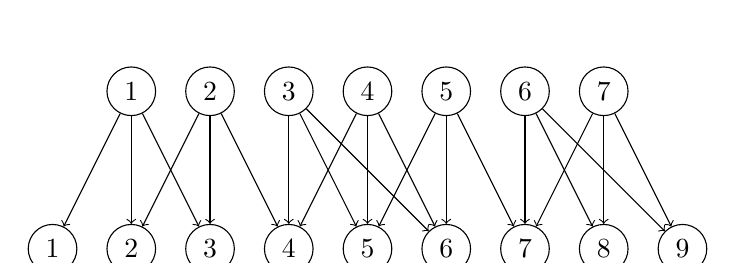
\begin{tikzpicture}              
            \node [circle, draw=black] (J1) at (3, 6) {$1$}; 
            \node [circle, draw=black] (J2) at (4, 6) {$2$}; 
            \node [circle, draw=black] (J3) at (5, 6) {$3$}; 
            \node [circle, draw=black] (J4) at (6, 6) {$4$}; 
            \node [circle, draw=black] (J5) at (7, 6) {$5$}; 
            \node [circle, draw=black] (J6) at (8, 6) {$6$}; 
            \node [circle, draw=black] (J7) at (9, 6) {$7$}; 
            
            \node [circle, draw=black] (T1) at (2, 4) {$1$}; 
            \node [circle, draw=black] (T2) at (3, 4) {$2$}; 
            \node [circle, draw=black] (T3) at (4, 4) {$3$}; 
            \node [circle, draw=black] (T4) at (5, 4) {$4$}; 
            \node [circle, draw=black] (T5) at (6, 4) {$5$}; 
            \node [circle, draw=black] (T6) at (7, 4) {$6$}; 
            \node [circle, draw=black] (T7) at (8, 4) {$7$}; 
            \node [circle, draw=black] (T8) at (9, 4) {$8$}; 
            \node [circle, draw=black] (T9) at (10, 4) {$9$};
            
            \draw [->] (J1) -- (T1); \draw [->] (J1) -- (T2); \draw [->] (J1) -- (T3); 
            \draw [->] (J2) -- (T2); \draw [->] (J2) -- (T3); \draw [->] (J2) -- (T4); 
            \draw [->] (J3) -- (T4); \draw [->] (J3) -- (T5); \draw [->] (J3) -- (T6);
            \draw [->] (J4) -- (T4); \draw [->] (J4) -- (T5); \draw [->] (J4) -- (T6); 
            \draw [->] (J5) -- (T5); \draw [->] (J5) -- (T6); \draw [->] (J5) -- (T7); 
            \draw [->] (J6) -- (T7); \draw [->] (J6) -- (T8); \draw [->] (J6) -- (T9); 
            \draw [->] (J7) -- (T7); \draw [->] (J7) -- (T8); \draw [->] (J7) -- (T9); 
        \end{tikzpicture} 
    \end{center}
    We find matchings and remove them until all edges are coloured. 
    \begin{center}
        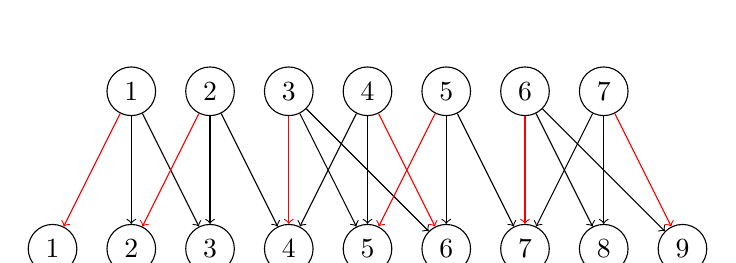
\begin{tikzpicture}              
            \node [circle, draw=black] (J1) at (3, 6) {$1$}; 
            \node [circle, draw=black] (J2) at (4, 6) {$2$}; 
            \node [circle, draw=black] (J3) at (5, 6) {$3$}; 
            \node [circle, draw=black] (J4) at (6, 6) {$4$}; 
            \node [circle, draw=black] (J5) at (7, 6) {$5$}; 
            \node [circle, draw=black] (J6) at (8, 6) {$6$}; 
            \node [circle, draw=black] (J7) at (9, 6) {$7$}; 
            
            \node [circle, draw=black] (T1) at (2, 4) {$1$}; 
            \node [circle, draw=black] (T2) at (3, 4) {$2$}; 
            \node [circle, draw=black] (T3) at (4, 4) {$3$}; 
            \node [circle, draw=black] (T4) at (5, 4) {$4$}; 
            \node [circle, draw=black] (T5) at (6, 4) {$5$}; 
            \node [circle, draw=black] (T6) at (7, 4) {$6$}; 
            \node [circle, draw=black] (T7) at (8, 4) {$7$}; 
            \node [circle, draw=black] (T8) at (9, 4) {$8$}; 
            \node [circle, draw=black] (T9) at (10, 4) {$9$};
            
            \draw [->, color=red] (J1) -- (T1); \draw [->] (J1) -- (T2); \draw [->] (J1) -- (T3); 
            \draw [->, color=red] (J2) -- (T2); \draw [->] (J2) -- (T3); \draw [->] (J2) -- (T4); 
            \draw [->, color=red] (J3) -- (T4); \draw [->] (J3) -- (T5); \draw [->] (J3) -- (T6);
            \draw [->] (J4) -- (T4); \draw [->] (J4) -- (T5); \draw [->, color=red] (J4) -- (T6); 
            \draw [->, color=red] (J5) -- (T5); \draw [->] (J5) -- (T6); \draw [->] (J5) -- (T7); 
            \draw [->, color=red] (J6) -- (T7); \draw [->] (J6) -- (T8); \draw [->] (J6) -- (T9); 
            \draw [->] (J7) -- (T7); \draw [->] (J7) -- (T8); \draw [->, color=red] (J7) -- (T9); 
        \end{tikzpicture} 
    \end{center}
    \begin{center}
        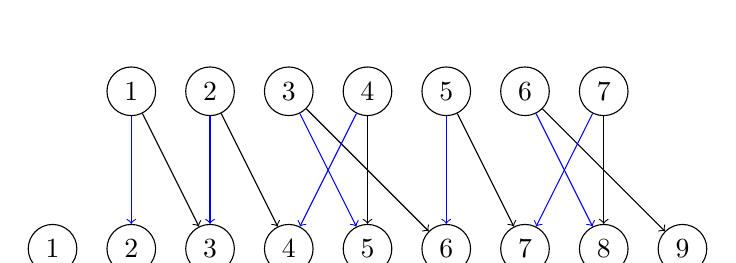
\begin{tikzpicture}              
            \node [circle, draw=black] (J1) at (3, 6) {$1$}; 
            \node [circle, draw=black] (J2) at (4, 6) {$2$}; 
            \node [circle, draw=black] (J3) at (5, 6) {$3$}; 
            \node [circle, draw=black] (J4) at (6, 6) {$4$}; 
            \node [circle, draw=black] (J5) at (7, 6) {$5$}; 
            \node [circle, draw=black] (J6) at (8, 6) {$6$}; 
            \node [circle, draw=black] (J7) at (9, 6) {$7$}; 
            
            \node [circle, draw=black] (T1) at (2, 4) {$1$}; 
            \node [circle, draw=black] (T2) at (3, 4) {$2$}; 
            \node [circle, draw=black] (T3) at (4, 4) {$3$}; 
            \node [circle, draw=black] (T4) at (5, 4) {$4$}; 
            \node [circle, draw=black] (T5) at (6, 4) {$5$}; 
            \node [circle, draw=black] (T6) at (7, 4) {$6$}; 
            \node [circle, draw=black] (T7) at (8, 4) {$7$}; 
            \node [circle, draw=black] (T8) at (9, 4) {$8$}; 
            \node [circle, draw=black] (T9) at (10, 4) {$9$};
            
            \draw [->, color=blue] (J1) -- (T2); \draw [->] (J1) -- (T3); 
            \draw [->, color=blue] (J2) -- (T3); \draw [->] (J2) -- (T4); 
            \draw [->, color=blue] (J3) -- (T5); \draw [->] (J3) -- (T6);
            \draw [->, color=blue] (J4) -- (T4); \draw [->] (J4) -- (T5); 
            \draw [->, color=blue] (J5) -- (T6); \draw [->] (J5) -- (T7); 
            \draw [->, color=blue] (J6) -- (T8); \draw [->] (J6) -- (T9); 
            \draw [->, color=blue] (J7) -- (T7); \draw [->] (J7) -- (T8); 
        \end{tikzpicture} 
    \end{center}
    \begin{center}
        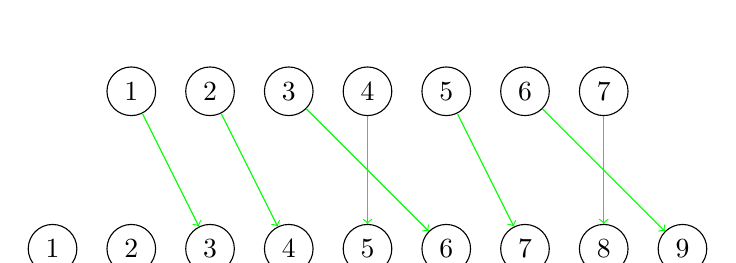
\begin{tikzpicture}              
            \node [circle, draw=black] (J1) at (3, 6) {$1$}; 
            \node [circle, draw=black] (J2) at (4, 6) {$2$}; 
            \node [circle, draw=black] (J3) at (5, 6) {$3$}; 
            \node [circle, draw=black] (J4) at (6, 6) {$4$}; 
            \node [circle, draw=black] (J5) at (7, 6) {$5$}; 
            \node [circle, draw=black] (J6) at (8, 6) {$6$}; 
            \node [circle, draw=black] (J7) at (9, 6) {$7$}; 
            
            \node [circle, draw=black] (T1) at (2, 4) {$1$}; 
            \node [circle, draw=black] (T2) at (3, 4) {$2$}; 
            \node [circle, draw=black] (T3) at (4, 4) {$3$}; 
            \node [circle, draw=black] (T4) at (5, 4) {$4$}; 
            \node [circle, draw=black] (T5) at (6, 4) {$5$}; 
            \node [circle, draw=black] (T6) at (7, 4) {$6$}; 
            \node [circle, draw=black] (T7) at (8, 4) {$7$}; 
            \node [circle, draw=black] (T8) at (9, 4) {$8$}; 
            \node [circle, draw=black] (T9) at (10, 4) {$9$};
            
            \draw [->, color=green] (J1) -- (T3); 
            \draw [->, color=green] (J2) -- (T4); 
            \draw [->, color=green] (J3) -- (T6);
            \draw [->, color=green] (J4) -- (T5); 
            \draw [->, color=green] (J5) -- (T7); 
            \draw [->, color=green] (J6) -- (T9); 
            \draw [->, color=green] (J7) -- (T8); 
        \end{tikzpicture} 
    \end{center}
    Letting red denote machine $1$, blue denote machine $2$, and 
    green denote machine $3$, we are led to the following schedule
    which has $L_{\max} = 1$. 
    \begin{center} 
        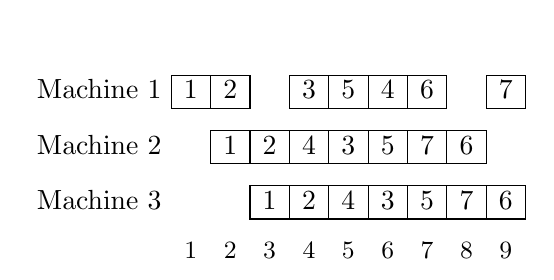
\begin{tikzpicture}[/pgfgantt/y unit chart=0.7cm] 
            \begin{ganttchart}[
                title/.style={draw=none},
                canvas/.append style={draw=none}, 
                bar top shift=0.1, bar height=0.6,
                y unit title=0.7cm,
            ]{1}{9}
                \ganttbar{Machine 1}{1}{1} \ganttbar[inline]{1}{1}{1} \ganttbar[inline]{2}{2}{2} 
                \ganttbar[inline]{3}{4}{4} \ganttbar[inline]{5}{5}{5} \ganttbar[inline]{4}{6}{6} 
                \ganttbar[inline]{6}{7}{7} \ganttbar[inline]{7}{9}{9} \\ 
                \ganttbar{Machine 2}{2}{2} \ganttbar[inline]{1}{2}{2} \ganttbar[inline]{2}{3}{3}
                \ganttbar[inline]{4}{4}{4} \ganttbar[inline]{3}{5}{5} \ganttbar[inline]{5}{6}{6} 
                \ganttbar[inline]{7}{7}{7} \ganttbar[inline]{6}{8}{8} \\ 
                \ganttbar{Machine 3}{3}{3} \ganttbar[inline]{1}{3}{3} \ganttbar[inline]{2}{4}{4} 
                \ganttbar[inline]{4}{5}{5} \ganttbar[inline]{3}{6}{6} \ganttbar[inline]{5}{7}{7} 
                \ganttbar[inline]{7}{8}{8} \ganttbar[inline]{6}{9}{9} \\ 
                \gantttitlelist{1,...,9}{1} 
            \end{ganttchart}
        \end{tikzpicture}
    \end{center}
    \vspace{-0.4cm}
    Note that we have not verified at this point whether or not there is a 
    feasible schedule for $L = 0$. But by running this algorithm again 
    with this parameter, we can find a certificate of infeasibility 
    for the network flow problem. For example, one could determine 
    the dual of the transportation model we discussed above and show 
    that the dual is unbounded, which implies that the transportation 
    model is infeasible. Thus, there does not exist a schedule 
    in which every job is completed on time.
\end{exmp}\newpage
\section{Job Shops} \label{sec:9}
In a job shop, each job has its own route to follow through the machines. 
This is a more general case of the flow job, where each job followed 
the same route. We will focus on the makespan objective, and describe 
formulations of the job shop problem as disjunctive graphs. We then 
describe two approaches to solving the problem: a branch and bound approach, 
and a popular and effective heuristic. 

\subsection{Disjunctive Programming and Branch and Bound} \label{subsec:9.1}
We first say a few words on active schedules and semi-active schedules.

\begin{defn}{defn:9.1}
    We say that a schedule is {\bf active} if it is not possible to 
    construct another schedule by changing the order of processing on the 
    machines and having at least one task finishing earlier without 
    any task finishing later. (Informally, when a schedule is active and there 
    are ``holes'' in the Gantt chart, then we cannot fit any of the later jobs 
    into these holes.)

    We say that a schedule is {\bf semi-active} if no task can be 
    completed earlier without changing the order of processing on any 
    one of the machines. 
\end{defn}

\begin{exmp}{exmp:9.2}
    Consider the following job shop with $3$ machines and $2$ jobs, where 
    both jobs must be processed last on machine $2$.  
    \begin{align*}
        \begin{array}{c|c|c}
            \text{Job} & \text{Machine Sequence} & \text{Processing Times} \\ \hline 
            1 & 1, 2 & p_{11} = 1,\, p_{21} = 3 \\ 
            2 & 3, 2 & p_{32} = 2,\, p_{22} = 3
        \end{array}
    \end{align*}
    Then the following schedule is active as reversing the sequence 
    of the two jobs on machine $2$ postpones the processing of job $2$. 
    However, the schedule is neither non-delay nor optimal, since machine 
    $2$ remains idle until time $2$ while there is a job available for processing 
    at time $1$. 
    \begin{center} 
        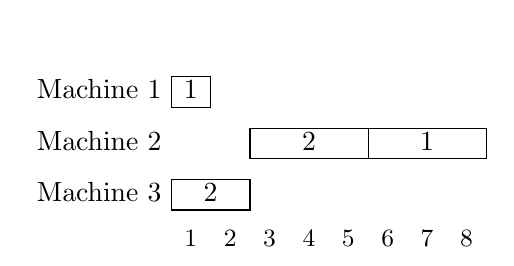
\begin{tikzpicture}[/pgfgantt/y unit chart=0.65cm] 
            \begin{ganttchart}[
                title/.style={draw=none},
                canvas/.append style={draw=none}, 
                bar top shift=0.1, bar height=0.6,
                y unit title=0.65cm
            ]{1}{8}
                \ganttbar{Machine 1}{1}{1} \ganttbar[inline]{1}{1}{1} \\ 
                \ganttbar{Machine 2}{3}{5} \ganttbar[inline]{2}{3}{5} \ganttbar[inline]{1}{6}{8} \\ 
                \ganttbar{Machine 3}{1}{2} \ganttbar[inline]{2}{1}{2} \\ 
                \gantttitlelist{1,...,8}{1}
            \end{ganttchart}
        \end{tikzpicture}
    \end{center} 
    \vspace{-0.5cm}
    Consider now the job shop which has the same routing as above but 
    the processing times are now $p_{11} = p_{21} = 1$ and 
    $p_{32} = p_{22} = 2$. The following schedule is a semi-active schedule.
    However, it is not active as job $1$ can be processed on machine $2$ 
    without delaying the processing of job $2$ on machine $2$.  
    \begin{center} 
        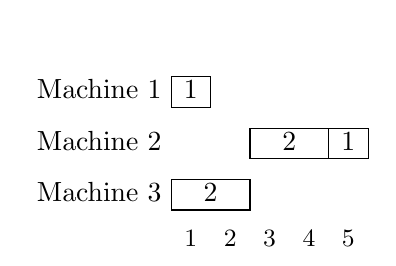
\begin{tikzpicture}[/pgfgantt/y unit chart=0.65cm] 
            \begin{ganttchart}[
                title/.style={draw=none},
                canvas/.append style={draw=none}, 
                bar top shift=0.1, bar height=0.6,
                y unit title=0.65cm
            ]{1}{5}
                \ganttbar{Machine 1}{1}{1} \ganttbar[inline]{1}{1}{1} \\ 
                \ganttbar{Machine 2}{3}{4} \ganttbar[inline]{2}{3}{4} \ganttbar[inline]{1}{5}{5} \\ 
                \ganttbar{Machine 3}{1}{2} \ganttbar[inline]{2}{1}{2} \\ 
                \gantttitlelist{1,...,5}{1}
            \end{ganttchart}
        \end{tikzpicture}
    \end{center} 
    \vspace{-0.4cm}
\end{exmp}

The $(J_m~||~C_{\max})$ can be represented using a nice disjunctive graph. 
Consider a directed graph $G$ with a set of nodes $N$ and two sets of 
arcs $A$ and $B$. The nodes $N$ correspond to all the operations $(i, j)$ 
that must be performed on the $n$ jobs. The {\bf conjunctive} arcs $A$
represent the routes of the jobs. That is, if the arc $(i, j) \to (k, j)$ 
is a part of $A$, then job $j$ has to be processed on machine $i$ before 
it is processed on machine $k$. Two operations that belong to different 
jobs but the same machine are joined by a {\bf disjunctive} arc, 
which has no direction given to it yet. The disjunctive arcs $B$ form 
$m$ cliques for each machine, and all operations in the same clique 
have to be done on the same machine. Each node has cost the processing 
time of the operation represented by that node. In addition, there is a 
source $0$ and a sink $\star$, which are dummy nodes. The source node $0$ 
has $n$ conjunctive arcs emanating to the first operations of the $n$ jobs, 
and the sink node has $n$ conjunctive arcs coming in from the last operations. 
This graph is denoted $G = (N, A, B)$. 
\begin{center}
    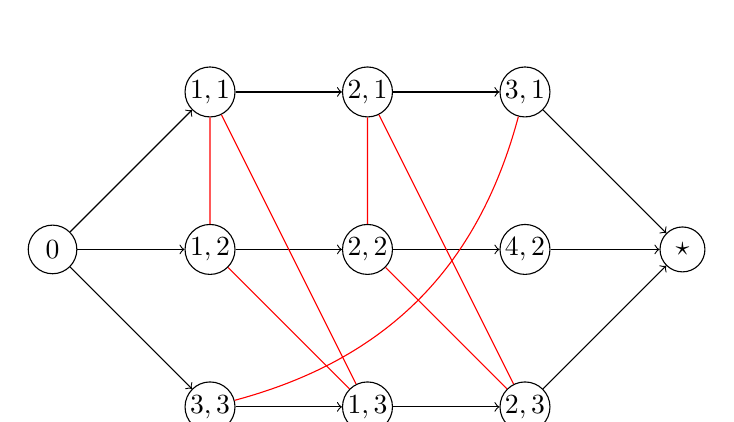
\begin{tikzpicture}              
        \node [circle, draw=black] (0) at (0, 0) {$0$}; 
        \node [circle, draw=black, inner sep=0.5pt] (11) at (2, 2) {$1, 1$}; 
        \node [circle, draw=black, inner sep=0.5pt] (12) at (2, 0) {$1, 2$}; 
        \node [circle, draw=black, inner sep=0.5pt] (33) at (2, -2) {$3, 3$}; 
        \node [circle, draw=black, inner sep=0.5pt] (21) at (4, 2) {$2, 1$}; 
        \node [circle, draw=black, inner sep=0.5pt] (22) at (4, 0) {$2, 2$}; 
        \node [circle, draw=black, inner sep=0.5pt] (13) at (4, -2) {$1, 3$}; 
        \node [circle, draw=black, inner sep=0.5pt] (31) at (6, 2) {$3, 1$}; 
        \node [circle, draw=black, inner sep=0.5pt] (42) at (6, 0) {$4, 2$}; 
        \node [circle, draw=black, inner sep=0.5pt] (23) at (6, -2) {$2, 3$};
        \node [circle, draw=black] (star) at (8, 0) {$\star$};
        
        \draw [->] (0) -- (11); \draw [->] (0) -- (12); \draw [->] (0) -- (33);
        \draw [->] (11) -- (21); \draw [->] (21) -- (31); \draw [->] (31) -- (star);
        \draw [->] (12) -- (22); \draw [->] (22) -- (42); \draw [->] (42) -- (star);
        \draw [->] (33) -- (13); \draw [->] (13) -- (23); \draw [->] (23) -- (star);
        \draw [color=red] (11) -- (12) -- (13) -- (11);
        \draw [color=red] (21) -- (22) -- (23) -- (21);
        \draw [red, bend right] (33) edge (31);
    \end{tikzpicture} 
\end{center}

A feasible schedule corresponds to selecting a direction for each 
disjunctive arc such that the resulting graph is acyclic. This implies that 
the selection of direction for each clique must be acyclic. Such a 
selection determines the sequence in which the operations are to be 
performed on that machine. If $D$ denotes the subset of the selected 
disjunctive arcs and $G(D)$ is the graph containing the conjunctive 
arcs together with the selected disjunctive arcs, then $D$ corresponds 
to a feasible schedule if and only if $G(D)$ contains no directed cycles. 

The makespan of a feasible schedule is determined by the longest path 
in $G(D)$ from the source $0$ to the sink $\star$. This longest path 
consists of a set of operations of which the first starts at time $0$ 
and the last finishes at the time of the makespan. Each operation 
on this path is immediately followed by either the next operation on the 
same machine or the next operation of the same job on another machine. 
Thus, the problem of minimizing the makespan is reduced to finding a 
selection of disjunctive arcs that minimizes the length of the longest 
path (that is, the {\bf critical} path). 

We now give a so-called disjunctive programming formulation for minimizing 
the makespan in a job shop. This formulation is closely related to 
the disjunctive graph representation of the job shop. 

Let $y_{ij}$ denote the starting time of operation $(i, j)$. Recall 
that the set $N$ denotes the set of all operations $(i, j)$, and 
the set $A$ contains all routing constraints $(i, j) \to (k, j)$ that 
require job $j$ to be processed on machine $i$ before it is processed on 
machine $k$. Then the following program minimizes the makespan. 
\begin{align*}
    \min\quad & C_{\max} \\ 
    \text{s.t.}\quad & y_{kj} - y_{ij} \geq p_{ij}, && \text{for all } (i, j) \to (k, j) \in A, \\ 
    & C_{\max} - y_{ij} \geq p_{ij}, && \text{for all } (i, j) \in N, \\ 
    & y_{ij} - y_{i\ell} \geq p_{i\ell} \text{ or } y_{i\ell} - y_{ij} \geq p_{ij}, 
        && \text{for all } (i, \ell) \text{ and } (i, j),\; i = 1, \dots, m, \\ 
    & y_{ij} \geq 0, && \text{for all } (i, j) \in N. 
\end{align*}
The first set of constraints ensure that operation $(k, j)$ cannot start before 
operation $(i, j)$ is completed. The third set of constraints are called the 
disjunctive constraints, and ensure that some ordering exists among operations 
of different jobs that have to be processed on the same machine. Because of 
these constraints, this formulation is referred to as a disjunctive programming 
formulation. 

Of course, the fact that a scheduling problem can be formulated as a 
disjunctive program does not imply that there is a standard solution 
procedure available that will work satisfactorily. Minimizing the makespan 
in a job shop is a very hard problem and solution procedures are either 
based on enumeration or on heuristics. 

To obtain an optimal solution, we require branch and bound methods. 
The branching as well as the bounding procedures that are applicable to this 
problem are usually of a special design. In this case, we will consider 
active schedules. It can be shown that there exists among all possible 
schedules an active schedule that minimizes the makespan. 

A branching schedule that is often used is based on the generation of 
all active schedules. All such active schedules can be generated by a 
simple algorithm. In this algorithm: 
\begin{itemize}
    \item $\Omega$ denotes the set of all operations of which all 
    predecessors have already been scheduled; 
    \item $r_{ij}$ denotes the earliest possible starting time of operation 
    $(i, j)$ in $\Omega$; and 
    \item $\Omega'$ is a subset of $\Omega$. 
\end{itemize}

\begin{algo}[Generation of All Active Schedules]{algo:9.3}
    \begin{enumerate}
        \item (Initial Condition) Let $\Omega$ contain the first operation 
        of each job, and let $r_{ij} = 0$ for all $(i, j) \in \Omega$. 

        \item (Machine Selection) For the current partial schedule, compute 
        \[ t(\Omega) = \min_{(i, j) \in \Omega} \{r_{ij} + p_{ij}\}, \] 
        and let $i^*$ denote the machine on which the minimum is achieved. 

        \item (Branching) Let $\Omega'$ denote the set of all operations 
        $(i^*, j) \in \Omega$ on machine $i^*$ such that 
        \[ r_{i^*j} < t(\Omega). \] 
        For each operation in $\Omega'$, consider an (extended) partial 
        schedule with that operation as the next one on machine $i^*$. 
        
        For each such (extended) partial schedule, delete the operation 
        from $\Omega$, include its immediate follower in $\Omega$, 
        and return to Step 2. 
    \end{enumerate}
\end{algo}

Algorithm~\ref{algo:9.3} is the basis for the branching process. Step 3 
performs the branching from the node that is characterized by the 
current partial schedule; the number of branches is equal to the 
number of operations in $\Omega'$. Using this algorithm, one can 
generate the entire tree. The nodes at the very bottom of the tree 
correspond to all the active schedules. 

A node $V$ in the tree corresponds to a partial schedule, and the partial 
schedule is characterized by a selection of disjunctive arcs that 
correspond to the order in which all the predecessors of a given set 
$\Omega$ have been scheduled. 
Note that each branch corresponds to the choice of an operation $(i^*, j)$ 
for a machine $i^*$. In particular, this fixes directions to the disjunctive 
arcs $(i^*, j) \to (i^*, k)$ for all unscheduled operations $(i^*, k)$. 
Let $D'$ denote the set of disjunctive arcs selected at the newly created 
node. Refer to the graph that includes all the conjunctive arcs and the 
the arcs in $D'$ as $G(D')$. The number of branches coming out of node $V$ 
is equal to the number of operations in $\Omega'$. 

To find a lower bound for the makespan at node $V'$, consider the graph 
$G(D')$. The length of the critical path in this graph already results 
in a lower bound for the makespan at node $V'$. Call this lower bound 
$\text{LB}(V')$. We can obtain a better (higher) lower bound as follows. 

Consider machine $i$ and assume that all \emph{other} machines are allowed 
to process, at any point in time, multiple operations simultaneously. 
(Since not all disjunctive arcs have been selected yet in $G(D')$, it 
may be the case that at some points in time, multiple operations 
require processing on the same machine at the same time.) However, machine $i$ 
must process its operations one after another. 

\begin{itemize}
    \item First, compute the earliest possible starting times $r_{ij}$ 
    of all the operations $(i, j)$ on machine $i$. This is done by 
    finding the length of the longest path from the source node $0$ to 
    node $(i, j)$ in $G(D')$, excluding the cost of node $(i, j)$ itself. 

    \item Second, for each operation $(i, j)$ on machine $i$, compute the 
    minimum amount of time $q_{ij}$ needed between the completion of operation $(i, j)$ 
    and the lower bound $\text{LB}(V')$. This is done by determining the 
    longest path from node $(i, j)$ to the sink $\star$ in $G(D')$, again 
    excluding the cost of node $(i, j)$ itself. 

    \item This amount of time, together with the lower bound on the makespan, 
    translates into a due date $d_{ij}$ for operation $(i, j)$; that is, 
    we have $d_{ij} = \text{LB}(V') - q_{ij}$. 
\end{itemize}

Consider now the problem of sequencing the operations on machine $i$ 
as a single machine problem with jobs arriving at different release dates, 
no preemptions allowed, and the maximum lateness as the objective 
to be minimized. This is the $(1~|~r_j~|~L_{\max})$ problem. Even though 
this problem is strongly $\NP$-hard, there are relatively effective 
algorithms that generate good solutions, and it is not hard to 
find optimal schedules by inspection when the number of jobs is small. 

The optimal sequence obtained for this problem implies a selection of 
disjunctive arcs that can be (temporarily) added to $D'$. This may then 
lead to a longer overall critical path in the graph, a larger makespan, 
and thus a better (higher) lower bound for the node $V'$. At node $V'$, 
this can be done for each of the $m$ machines separately. The largest 
makespan obtained in this way can be used as a lower bound for node $V'$. 
Of course, the temporary disjunctive arcs inserted to obtain the lower 
bound are deleted as soon as the best lower bound is determined. 

Although it seems somewhat of a burden to have to solve $m$ strongly 
$\NP$-hard scheduling problems in order to obtain one lower bound 
for another strongly $\NP$-hard problem, this type of bounding procedure 
has performed reasonably well in computational experiments. 

\begin{exmp}{exmp:9.4}
    Consider the following instance of $(J_4~||~C_{\max})$ with $3$ jobs. 
    \begin{align*}
        \begin{array}{c|c|c}
            \text{Job} & \text{Machine Sequence} & \text{Processing Times} \\ \hline 
            1 & 1, 2, 3 & p_{11} = 10,\, p_{21} = 8,\, p_{31} = 4 \\ 
            2 & 2, 1, 4, 3 & p_{22} = 8,\, p_{12} = 3,\, p_{42} = 5,\, p_{32} = 6 \\ 
            3 & 1, 2, 4 & p_{13} = 4,\, p_{23} = 7,\, p_{43} = 3
        \end{array}
    \end{align*}
    This instance can be depicted using the following disjunctive graph. 
    The longest path is $0 \to (2, 2) \to (1, 2) \to (4, 2) \to (3, 2) \to 
    \star$ and so we immediately get a lower bound of $22$ on the makespan. 
    \begin{center}
        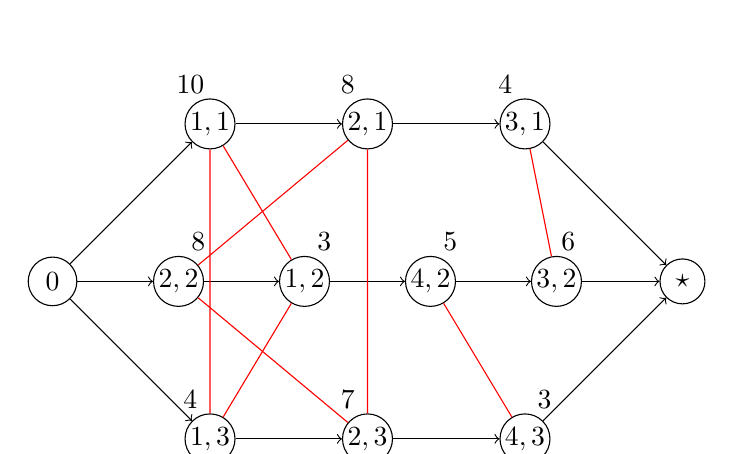
\begin{tikzpicture}              
            \node [circle, draw=black] (0) at (0, 0) {$0$}; 
            \node [circle, draw=black, inner sep=0.5pt] (11) at (2, 2) {$1, 1$}; 
            \node [circle, draw=black, inner sep=0.5pt] (21) at (4, 2) {$2, 1$}; 
            \node [circle, draw=black, inner sep=0.5pt] (31) at (6, 2) {$3, 1$}; 

            \node [circle, draw=black, inner sep=0.5pt] (22) at (1.6, 0) {$2, 2$}; 
            \node [circle, draw=black, inner sep=0.5pt] (12) at (3.2, 0) {$1, 2$};
            \node [circle, draw=black, inner sep=0.5pt] (42) at (4.8, 0) {$4, 2$};
            \node [circle, draw=black, inner sep=0.5pt] (32) at (6.4, 0) {$3, 2$};

            \node [circle, draw=black, inner sep=0.5pt] (13) at (2, -2) {$1, 3$}; 
            \node [circle, draw=black, inner sep=0.5pt] (23) at (4, -2) {$2, 3$}; 
            \node [circle, draw=black, inner sep=0.5pt] (43) at (6, -2) {$4, 3$};

            \node (p11) at (1.75, 2.5) {$10$}; 
            \node (p21) at (3.75, 2.5) {$8$}; 
            \node (p31) at (5.75, 2.5) {$4$}; 

            \node (p22) at (1.85, 0.5) {$8$};
            \node (p12) at (3.45, 0.5) {$3$}; 
            \node (p42) at (5.05, 0.5) {$5$}; 
            \node (p32) at (6.55, 0.5) {$6$}; 

            \node (p13) at (1.75, -1.5) {$4$}; 
            \node (p23) at (3.75, -1.5) {$7$};
            \node (p43) at (6.25, -1.5) {$3$};

            \node [circle, draw=black] (star) at (8, 0) {$\star$};
            
            \draw [->] (0) -- (11); \draw [->] (0) -- (22); \draw [->] (0) -- (13);
            \draw [->] (11) -- (21); \draw [->] (21) -- (31); \draw [->] (31) -- (star);
            \draw [->] (22) -- (12); \draw [->] (12) -- (42); \draw [->] (42) -- (32); \draw [->] (32) -- (star);
            \draw [->] (13) -- (23); \draw [->] (23) -- (43); \draw [->] (43) -- (star);

            \draw [color=red] (11) -- (12) -- (13) -- (11);
            \draw [color=red] (21) -- (22) -- (23) -- (21);
            \draw [color=red] (31) edge (32);
            \draw [color=red] (42) edge (43);
        \end{tikzpicture} 
    \end{center}
    Then applying Algorithm~\ref{algo:9.3} gives us 
    \begin{align*}
        \Omega &= \{(1, 1), (2, 2), (1, 3)\}, \\ 
        t(\Omega) &= \min\{0 + 10, 0 + 8, 0 + 4\} = 4, \\ 
        i^* &= 1, \\ 
        \Omega' &= \{(1, 1), (1, 3)\}. 
    \end{align*}
    So at level $1$, there are two nodes of interest: one corresponding to 
    operation $(1, 1)$ being processed first on machine $1$, and the other 
    corresponding to operation $(1, 3)$ being processed first on machine $1$.
    
    If operation $(1, 1)$ is scheduled first, we add directions to the 
    following blue disjunctive arcs to the graph. 
    \begin{center}
        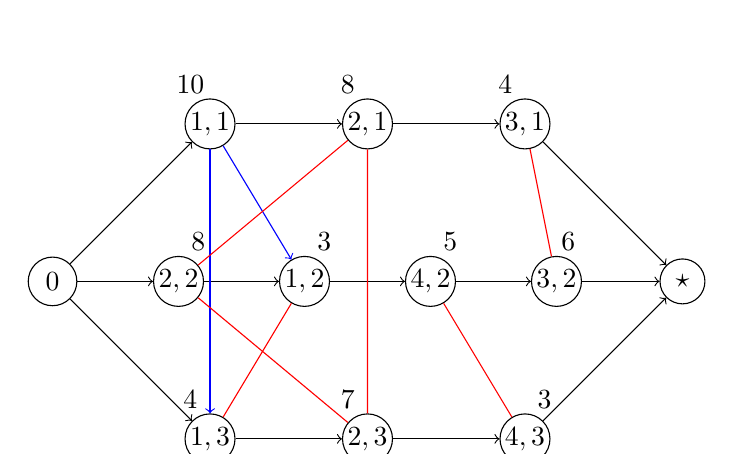
\begin{tikzpicture}              
            \node [circle, draw=black] (0) at (0, 0) {$0$}; 
            \node [circle, draw=black, inner sep=0.5pt] (11) at (2, 2) {$1, 1$}; 
            \node [circle, draw=black, inner sep=0.5pt] (21) at (4, 2) {$2, 1$}; 
            \node [circle, draw=black, inner sep=0.5pt] (31) at (6, 2) {$3, 1$}; 

            \node [circle, draw=black, inner sep=0.5pt] (22) at (1.6, 0) {$2, 2$}; 
            \node [circle, draw=black, inner sep=0.5pt] (12) at (3.2, 0) {$1, 2$};
            \node [circle, draw=black, inner sep=0.5pt] (42) at (4.8, 0) {$4, 2$};
            \node [circle, draw=black, inner sep=0.5pt] (32) at (6.4, 0) {$3, 2$};

            \node [circle, draw=black, inner sep=0.5pt] (13) at (2, -2) {$1, 3$}; 
            \node [circle, draw=black, inner sep=0.5pt] (23) at (4, -2) {$2, 3$}; 
            \node [circle, draw=black, inner sep=0.5pt] (43) at (6, -2) {$4, 3$};

            \node (p11) at (1.75, 2.5) {$10$}; 
            \node (p21) at (3.75, 2.5) {$8$}; 
            \node (p31) at (5.75, 2.5) {$4$}; 

            \node (p22) at (1.85, 0.5) {$8$};
            \node (p12) at (3.45, 0.5) {$3$}; 
            \node (p42) at (5.05, 0.5) {$5$}; 
            \node (p32) at (6.55, 0.5) {$6$}; 

            \node (p13) at (1.75, -1.5) {$4$}; 
            \node (p23) at (3.75, -1.5) {$7$};
            \node (p43) at (6.25, -1.5) {$3$};

            \node [circle, draw=black] (star) at (8, 0) {$\star$};
            
            \draw [->] (0) -- (11); \draw [->] (0) -- (22); \draw [->] (0) -- (13);
            \draw [->] (11) -- (21); \draw [->] (21) -- (31); \draw [->] (31) -- (star);
            \draw [->] (22) -- (12); \draw [->] (12) -- (42); \draw [->] (42) -- (32); \draw [->] (32) -- (star);
            \draw [->] (13) -- (23); \draw [->] (23) -- (43); \draw [->] (43) -- (star);

            \draw [->, color=blue] (11) -- (12);
            \draw [->, color=blue] (11) -- (13);
            \draw [color=red] (12) -- (13);
            \draw [color=red] (21) -- (22) -- (23) -- (21);
            \draw [color=red] (31) edge (32);
            \draw [color=red] (42) edge (43);
        \end{tikzpicture} 
    \end{center}
    This node is characterized by the two disjunctive arcs 
    $(1, 1) \to (1, 2)$ and $(1, 1) \to (1, 3)$. The addition of these 
    disjunctive arcs gives us a new longest path $0 \to (1, 1) \to (1, 2) 
    \to (4, 2) \to (3, 2) \to \star$ and a lower bound $\text{LB}(V') = 24$.
    In order to improve this lower bound, we can generate an instance of 
    $(1~|~r_j~|~L_{\max})$ for machine $1$. The release date of job $j$ 
    in this single machine problem is determined by the longest 
    path from the source node $0$ to the node $(1, j)$ excluding 
    the cost of node $(1, j)$, and the due date is computed by finding the 
    longest path from $(1, j)$ to the sink $\star$ (excluding the cost 
    of $(1, j)$ itself) and subtracting the resulting value from 
    $\text{LB}(V') = 24$. This leads us to the following instance 
    of $(1~|~r_j~|~L_{\max})$ for machine $1$. 
    \begin{align*}
        \begin{array}{c|ccc}
            j & 1 & 2 & 3 \\ \hline 
            p_{1j} & 10 & 3 & 4 \\ 
            r_{1j} & 0 & 10 & 10 \\ 
            d_{1j} & 10 & 13 & 14 
        \end{array}
    \end{align*}
    The sequence that minimizes $L_{\max}$ is $1, 2, 3$ with $L_{\max} = 3$, 
    implying that a lower bound for the makespan at the corresponding node 
    is $24 + 3 = 27$. We can also generate an instance of $(1~|~r_j~|~L_{\max})$ 
    for machine $2$ in the same way, and the release dates and due dates 
    are as follows. 
    \begin{align*}
        \begin{array}{c|ccc}
            j & 1 & 2 & 3 \\ \hline 
            p_{2j} & 8 & 8 & 7 \\ 
            r_{2j} & 10 & 0 & 14 \\ 
            d_{2j} & 20 & 10 & 21 
        \end{array}
    \end{align*}
    The optimal sequence is $2, 1, 3$ with $L_{\max} = 4$, so we get a 
    better lower bound of $24 + 4 = 28$ for the node with operation $(1, 1)$ 
    scheduled first. Analyzing machines $3$ and $4$ in the same way does not 
    yield a better lower bound. 

    The second node at level $1$ corresponds to operation $(1, 3)$ being scheduled
    first. In this case, we add the disjunctive arcs $(1, 3) \to (1, 1)$ 
    and $(1, 3) \to (1, 2)$ instead. 
    \begin{center}
        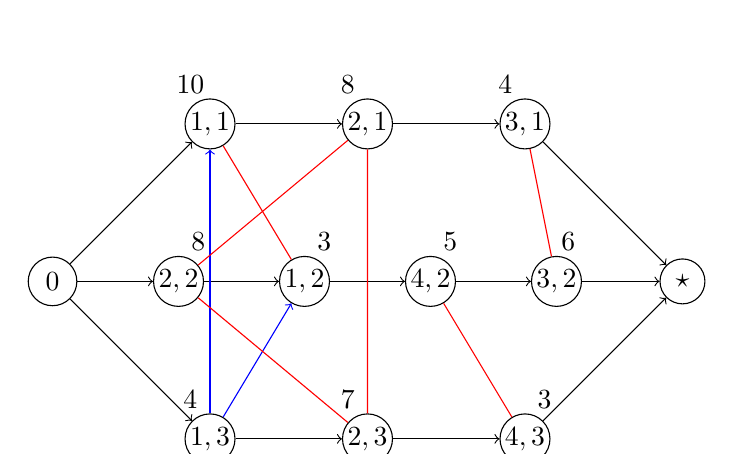
\begin{tikzpicture}              
            \node [circle, draw=black] (0) at (0, 0) {$0$}; 
            \node [circle, draw=black, inner sep=0.5pt] (11) at (2, 2) {$1, 1$}; 
            \node [circle, draw=black, inner sep=0.5pt] (21) at (4, 2) {$2, 1$}; 
            \node [circle, draw=black, inner sep=0.5pt] (31) at (6, 2) {$3, 1$}; 

            \node [circle, draw=black, inner sep=0.5pt] (22) at (1.6, 0) {$2, 2$}; 
            \node [circle, draw=black, inner sep=0.5pt] (12) at (3.2, 0) {$1, 2$};
            \node [circle, draw=black, inner sep=0.5pt] (42) at (4.8, 0) {$4, 2$};
            \node [circle, draw=black, inner sep=0.5pt] (32) at (6.4, 0) {$3, 2$};

            \node [circle, draw=black, inner sep=0.5pt] (13) at (2, -2) {$1, 3$}; 
            \node [circle, draw=black, inner sep=0.5pt] (23) at (4, -2) {$2, 3$}; 
            \node [circle, draw=black, inner sep=0.5pt] (43) at (6, -2) {$4, 3$};

            \node (p11) at (1.75, 2.5) {$10$}; 
            \node (p21) at (3.75, 2.5) {$8$}; 
            \node (p31) at (5.75, 2.5) {$4$}; 

            \node (p22) at (1.85, 0.5) {$8$};
            \node (p12) at (3.45, 0.5) {$3$}; 
            \node (p42) at (5.05, 0.5) {$5$}; 
            \node (p32) at (6.55, 0.5) {$6$}; 

            \node (p13) at (1.75, -1.5) {$4$}; 
            \node (p23) at (3.75, -1.5) {$7$};
            \node (p43) at (6.25, -1.5) {$3$};

            \node [circle, draw=black] (star) at (8, 0) {$\star$};
            
            \draw [->] (0) -- (11); \draw [->] (0) -- (22); \draw [->] (0) -- (13);
            \draw [->] (11) -- (21); \draw [->] (21) -- (31); \draw [->] (31) -- (star);
            \draw [->] (22) -- (12); \draw [->] (12) -- (42); \draw [->] (42) -- (32); \draw [->] (32) -- (star);
            \draw [->] (13) -- (23); \draw [->] (23) -- (43); \draw [->] (43) -- (star);

            \draw [->, color=blue] (13) -- (11);
            \draw [->, color=blue] (13) -- (12);
            \draw [color=red] (11) -- (12);
            \draw [color=red] (21) -- (22) -- (23) -- (21);
            \draw [color=red] (31) edge (32);
            \draw [color=red] (42) edge (43);
        \end{tikzpicture} 
    \end{center}
    We see that a lower bound on the makespan is $\text{LB}(V') = 26$ 
    via the longest path $0 \to (1, 3) \to (1, 1) \to (2, 1) \to (3, 1) 
    \to \star$. The associated maximum lateness problem for machine 
    $1$ has optimal sequence $3, 1, 2$ with $L_{\max} = 2$, which 
    implies that a lower bound for this node is $26 + 2 = 28$. Analyzing
    machines $2$, $3$, and $4$ in this way does not result in a better lower 
    bound. 

    The next step is to branch from node $(1, 1)$ at level $1$. Applying 
    Algorithm~\ref{algo:9.3} yields 
    \begin{align*}
        \Omega &= \{(2, 2), (2, 1), (1, 3)\}, \\ 
        t(\Omega) &= \min(0 + 8, 10 + 8, 10 + 4) = 8, \\ 
        i^* &= 2, \\ 
        \Omega' &= \{(2, 2)\}. 
    \end{align*}
    There is one node of interest at level 2, namely the node corresponding to 
    operation $(2, 2)$ being processed first on machine $2$. We add the
    disjunctive arcs $(2, 2) \to (2, 1)$ and $(2, 2) \to (2, 3)$ to the graph. 
    \begin{center}
        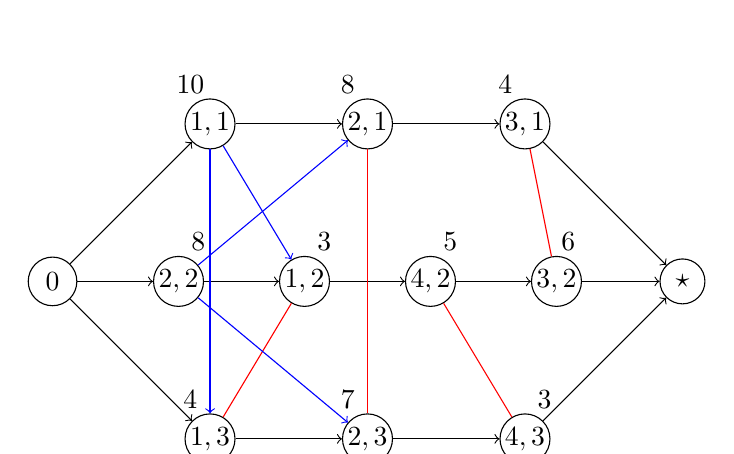
\begin{tikzpicture}              
            \node [circle, draw=black] (0) at (0, 0) {$0$}; 
            \node [circle, draw=black, inner sep=0.5pt] (11) at (2, 2) {$1, 1$}; 
            \node [circle, draw=black, inner sep=0.5pt] (21) at (4, 2) {$2, 1$}; 
            \node [circle, draw=black, inner sep=0.5pt] (31) at (6, 2) {$3, 1$}; 

            \node [circle, draw=black, inner sep=0.5pt] (22) at (1.6, 0) {$2, 2$}; 
            \node [circle, draw=black, inner sep=0.5pt] (12) at (3.2, 0) {$1, 2$};
            \node [circle, draw=black, inner sep=0.5pt] (42) at (4.8, 0) {$4, 2$};
            \node [circle, draw=black, inner sep=0.5pt] (32) at (6.4, 0) {$3, 2$};

            \node [circle, draw=black, inner sep=0.5pt] (13) at (2, -2) {$1, 3$}; 
            \node [circle, draw=black, inner sep=0.5pt] (23) at (4, -2) {$2, 3$}; 
            \node [circle, draw=black, inner sep=0.5pt] (43) at (6, -2) {$4, 3$};

            \node (p11) at (1.75, 2.5) {$10$}; 
            \node (p21) at (3.75, 2.5) {$8$}; 
            \node (p31) at (5.75, 2.5) {$4$}; 

            \node (p22) at (1.85, 0.5) {$8$};
            \node (p12) at (3.45, 0.5) {$3$}; 
            \node (p42) at (5.05, 0.5) {$5$}; 
            \node (p32) at (6.55, 0.5) {$6$}; 

            \node (p13) at (1.75, -1.5) {$4$}; 
            \node (p23) at (3.75, -1.5) {$7$};
            \node (p43) at (6.25, -1.5) {$3$};

            \node [circle, draw=black] (star) at (8, 0) {$\star$};
            
            \draw [->] (0) -- (11); \draw [->] (0) -- (22); \draw [->] (0) -- (13);
            \draw [->] (11) -- (21); \draw [->] (21) -- (31); \draw [->] (31) -- (star);
            \draw [->] (22) -- (12); \draw [->] (12) -- (42); \draw [->] (42) -- (32); \draw [->] (32) -- (star);
            \draw [->] (13) -- (23); \draw [->] (23) -- (43); \draw [->] (43) -- (star);

            \draw [->, color=blue] (11) -- (12);
            \draw [->, color=blue] (11) -- (13);
            \draw [color=red] (12) -- (13);
            \draw [->, color=blue] (22) -- (21);
            \draw [->, color=blue] (22) -- (23); 
            \draw [color=red] (21) -- (23);
            \draw [color=red] (31) edge (32);
            \draw [color=red] (42) edge (43);
        \end{tikzpicture} 
    \end{center}
    We have a lower bound $\text{LB}(V') = 28$ on this node because the 
    preceding node had this lower bound. This leads to an instance of 
    $(1~|~r_j~|~L_{\max})$ for machine $1$ with the following release 
    dates and due dates. 
    \begin{align*}
        \begin{array}{c|ccc}
            j & 1 & 2 & 3 \\ \hline 
            p_{1j} & 10 & 3 & 4 \\ 
            r_{1j} & 0 & 10 & 10 \\ 
            d_{1j} & 14 & 17 & 18 
        \end{array}
    \end{align*}
    The optimal sequence is $1, 3, 2$ with $L_{\max} = 0$. Then a 
    lower bound on this node is also $28 + 0 = 28$, and analyzing 
    machines $2$, $3$, and $4$ in the same way does not increase the 
    lower bound. 

    So far, the branch and bound tree is as follows. 
    \begin{center}
        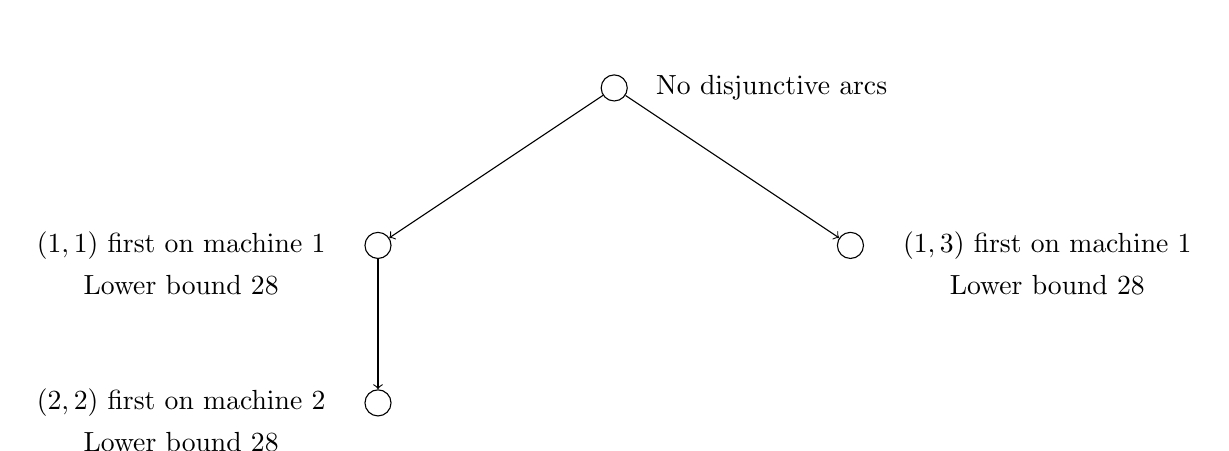
\begin{tikzpicture}              
            \node [circle, draw=black] (BB0) at (3, 8) {}; 
            \node [circle, draw=black] (BB11) at (0, 6) {}; 
            \node [circle, draw=black] (BB13) at (6, 6) {}; 
            \node [circle, draw=black] (BB22) at (0, 4) {};
            \node (DBB0) at (5, 8) {No disjunctive arcs}; 
            \node (DBB111) at (-2.5, 6) {$(1, 1)$ first on machine $1$};
            \node (DBB112) at (-2.5, 5.5) {Lower bound 28}; 
            \node (DBB131) at (8.5, 6) {$(1, 3)$ first on machine $1$};
            \node (DBB132) at (8.5, 5.5) {Lower bound 28}; 
            \node (DBB221) at (-2.5, 4) {$(2, 2)$ first on machine $2$};
            \node (DBB222) at (-2.5, 3.5) {Lower bound 28}; 
            
            \draw [->] (BB0) -- (BB11);
            \draw [->] (BB0) -- (BB13);
            \draw [->] (BB11) -- (BB22);
        \end{tikzpicture} 
    \end{center}
    Continuing the branch and bound procedure results in the following job 
    sequence for the four machines. 
    \begin{align*}
        \begin{array}{c|c}
            \text{Machine} & \text{Job Sequence} \\ \hline 
            1 & 1, 3, 2 \text{ or } 1, 2, 3 \\ 
            2 & 2, 1, 3 \\ 
            3 & 1, 2 \\ 
            4 & 2, 3
        \end{array}
    \end{align*}
    The makespan under this schedule is $28$, as seen in the following Gantt chart. 
    \begin{center} 
        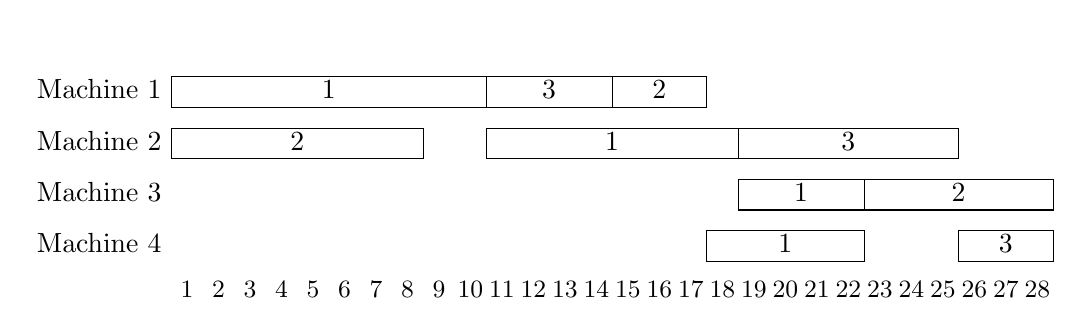
\begin{tikzpicture}[/pgfgantt/y unit chart=0.65cm] 
            \begin{ganttchart}[
                title/.style={draw=none},
                canvas/.append style={draw=none}, 
                bar top shift=0.1, bar height=0.6,
                y unit title=0.65cm,
                x unit=0.4cm
            ]{1}{28}
                \ganttbar{Machine 1}{1}{10} \ganttbar[inline]{1}{1}{10} \ganttbar[inline]{3}{11}{14} \ganttbar[inline]{2}{15}{17} \\ 
                \ganttbar{Machine 2}{1}{8} \ganttbar[inline]{2}{1}{8} \ganttbar[inline]{1}{11}{18} \ganttbar[inline]{3}{19}{25} \\ 
                \ganttbar{Machine 3}{19}{22} \ganttbar[inline]{1}{19}{22} \ganttbar[inline]{2}{23}{28} \\ 
                \ganttbar{Machine 4}{18}{22} \ganttbar[inline]{1}{18}{22} \ganttbar[inline]{3}{26}{28} \\ 
                \gantttitlelist{1,...,28}{1}
            \end{ganttchart}
        \end{tikzpicture}
    \end{center} 
    \vspace{-0.4cm}
\end{exmp}

While this approach is guaranteed to lead to an optimal schedule, the 
computation time is prohibitive with a large number of machines and a large 
number of jobs. With $20$ machines and $20$ jobs, it is already hard to 
find an optimal schedule. It is therefore necessarily to develop heuristics 
that lead to reasonably good schedules in a reasonably short time. The 
next section describes a well-known heuristic with an excellent track record.

\subsection{The Shifting Bottleneck Heuristic for Makespan} \label{subsec:9.2}
One of the most successful heuristic procedures developed for $(J_m~||~C_{\max})$ 
is the {\bf Shifting Bottleneck} heuristic. We denote the set of all 
machines by $M$. In the description of an iteration of the heuristic, 
it is assumed that in previous iterations, a selection of disjunctive 
arcs has already been fixed for a subset $M_0$ of machines. So for each 
of the machines in $M_0$, a sequence of operations has already been determined. 

An iteration determines which machine in $M \setminus M_0$ has to be included 
next into $M_0$. The sequence in which the operations on this machine 
have to be processed is also generated in this iteration. 

In order to select the machine to be included next in $M_0$, an attempt is 
made to determine which one of the machines yet to be scheduled would cause in 
some sense the severest disruption. To determine this, we consider the 
graph with only the directions of the disjunctive arcs of the machines in $M_0$
fixed. Call this graph $G'$. For the machines in $M \setminus M_0$, having 
no directions fixed on the disjunctive arcs implies that all operations 
on this machine can be done in parallel (as if the machine has infinite 
capacity, or equivalently, each one of the operations has the machine 
for itself). The graph $G'$ has one or more critical paths that determine 
the corresponding makespan. Call this makespan $C_{\max}(M_0)$. 

Let $i \in M \setminus M_0$, and suppose that operation $(i, j)$ has to be 
processed at a time window in which the release date and due date are 
determined by the critical (longest) paths in $G'$. That is, the 
release date is equal to the longest path in $G'$ from the source node $0$ 
to node $(i, j)$ (excluding the cost of $(i, j)$ itself), and the 
due date is equal to $C_{\max}(M_0)$ minus the longest path from 
node $(i, j)$ to the sink node $\star$ (again excluding the cost of 
$(i, j)$ itself). Then we can consider for each machine in $M \setminus M_0$ 
a separate $(1~|~r_j~|~L_{\max})$ problem. We stated earlier that this 
is strongly $\NP$-hard, but there are procedures that perform reasonably well.
The minimum $L_{\max}$ of the single machine problem corresponding to 
machine $i$ is denoted by $L_{\max}(i)$ and is a measure of the criticality of 
machine $i$. 

After solving all these single machine problems, the machine with the 
\emph{largest} maximum lateness is chosen. Among the remaining machines, 
this machine is in a sense the most critical or the ``bottleneck'' and therefore 
the one to be included next in $M_0$. Label this machine $k$, call its 
maximum lateness $L_{\max}(k)$, and schedule it according to the optimal 
solution obtained for the single machine problem associated with this 
machine. If the disjunctive arcs that specify the sequence of operations on 
machine $k$ are inserted in graph $G'$, then the makespan
of the current partial schedule increases by at least $L_{\max}(k)$; that is,
\[ C_{\max}(M_0 \cup \{k\}) \geq C_{\max}(M_0) + L_{\max}(k). \] 
Before starting the next iteration and determining the next machine to be
scheduled, one additional step has to be done within the current iteration. In
this additional step, all the machines in the original set $M_0$ are 
resequenced in order to see if the makespan can be reduced. That is, 
a machine, say $\ell$, is taken out of $M_0$ and a graph $G''$ is 
constructed by modifying $G'$ through the inclusion of the disjunctive arcs 
that specify the sequence of operations on machine $k$ and the exclusion 
of the disjunctive arcs associated with machine $\ell$. Then machine $\ell$ 
is resequenced by solving the corresponding $(1~|~r_j~|~L_{\max})$ 
problem with the release and due dates determined by the critical paths in 
$G''$. Resequencing each of the machines in the original set $M_0$ completes 
the iteration. 

Afterwards, the entire procedure is repeated and another machine is added 
to the current set $M_0 \cup \{k\}$. We summarize the algorithm as follows. 

\begin{algo}[Shifting Bottleneck Heuristic]{algo:9.5}
    \begin{enumerate}
        \item {\bf Initial conditions.} Set $M_0 = \varnothing$. The graph $G$ 
        has all the conjunctive arcs and no directions on the disjunctive arcs. 
        Set $C_{\max}(M_0)$ equal to the longest path in $G$. 

        \item {\bf Analysis of machines yet to be scheduled.} For each 
        machine in $M \setminus M_0$, do the following: 
        \begin{enumerate}[(a)]
            \item Generate an instance of $(1~|~r_j~|~L_{\max})$ with the 
            release date of operation $(i, j)$ determined by the longest 
            path in $G$ from the source node $0$ to node $(i, j)$ 
            (excluding $p_{ij}$), and the due date of operation $(i, j)$ 
            determined by $C_{\max}(M_0)$ minus the longest path in $G$ 
            from node $(i, j)$ to the sink $\star$ (excluding $p_{ij}$).
            \item Minimize $L_{\max}$ in each of these single machine 
            subproblems, and let $L_{\max}(i)$ denote the minimum 
            $L_{\max}$ in the subproblem corresponding to machine $i$. 
        \end{enumerate}

        \item {\bf Bottleneck selection and sequencing.} Let 
        \[ L_{\max}(k) = \max_{i \in M \setminus M_0} L_{\max}(i). \] 
        Sequence machine $k$ according to the sequence obtained in Step 2 
        for that machine. Insert all the corresponding disjunctive arcs 
        in $G$, and insert machine $k$ in $M_0$. 

        \item {\bf Resequencing of all earlier scheduled machines.} 
        For each machine $i \in M_0 \setminus \{k\}$, do the following: 
        \begin{enumerate}[(a)]
            \item Delete from $G$ the disjunctive arcs corresponding to machine $i$. 
            \item Formulate a $(1~|~r_j~|~L_{\max})$ subproblem for machine $i$ 
            with release dates and due dates of the operations determined by the 
            longest path calculations in $G$.
            \item Find the sequence which minimizes $L_{\max}(i)$ and insert the 
            corresponding disjunctive arcs in $G$. 
        \end{enumerate}

        \item {\bf Stopping criterion.} If $M_0 = M$, then stop. Otherwise, go back 
        to Step 2. 
    \end{enumerate}
\end{algo}

The structure of the shifting bottleneck heuristic shows the relationship between 
the bottleneck concept and more combinatorial concepts such as critical
(longest) path and maximum lateness. A critical path indicates the location
and the timing of a bottleneck. The maximum lateness gives an indication of
the amount by which the makespan increases if a machine is added to the set
of machines already scheduled.

Extensive numerical research has shown that the Shifting Bottleneck heuristic is extremely 
effective. When applied to a standard test problem with $10$
machines and $10$ jobs that had remained unsolved for more than $20$ years, the
heuristic obtained a very good solution very fast. This solution turned out to
be optimal after a branch and bound procedure found the same result and verified its 
optimality. The branch and bound approach, in contrast to the heuristic,
needed many hours of CPU time. The disadvantage of the heuristic is, of course,
that there is no guarantee that the solution it reaches is optimal.\newpage

\end{document}
